%% ----------------ATENCIÓ-----------------------
%% Aquest document està preparat per codificació 
%% UTF-8. Si es llegeix amb un editor 
%% preparat per una altra codificació alguns 
%% caràcters no es veuran correctament.
%%---------------------------------------------- 
%%
%% Aquest document vos pot servir de base per la
%% realització de la memòria del treball final de
%% grau. Es recomana seguir els consells que 
%% apareixen en els diferents comentaris del 
%% document. Convindrà mantenir l'estructura
%% d'aquest exemple i introduir canvis sols 
%% allà on s'indiqui.
%%
%%-----------------------------------------------
%%
%% La plantilla preparada per a la realització de
%% la memòria és la classe LaTeX TFGEPSUIB.cls
%% que es fonamenta en la classe memoir. Aquesta
%% emula alguns `packages` que, per tant, no serà
%% necessari incloure dins el vostre document. El
%% manual de memoir explica quins són aquests
%% paquets (per exemple booktabs, array, tabluarx). 
%% Per altra banda, TFGEPSUIB també carrega 
%% automàticament els paquets, fontenc, xcolor, 
%% graphicx i microtype.
%%
%%-----------------------------------------
%% Opcions de la classe TFGEPSUIB:
%%
%% Per defecte, la classe TFGEPSUIB suposa
%% que la memòria es redactarà en català i que 
%% els estudis són els de Grau en Enginyeria
%% telemàtica. 
%%
%% Si preferiu utilitzar el castellà o anglés
%% per a la redacció de la memòria podeu
%% fer-ho indicant-ho a les opcions.
%\documentclass[catalan]{TFGEPSUIB}
\documentclass[spanish,GINF]{TFGEPSUIB}
%%
%% Per indicar quins són els estudis pels quals
%% es redacta la memòria heu d'incloure una de
%% les següents opcions:
%%
%% GTEL - Grau en Enginyeria Telemàtica
%% GMAT - Grau de Matemàtiques
%% GINF - Grau d'Enginyeria Informàtica
%% GEDI - Grau d'Enginyeria d'Edificació
%% GELE - Grau d'Eng. Elec. Ind. i Automàtica
%% GAGR - Grau en Eng. Agroali. i del Medi Rural
%%
%% Per escriure la memòria en castellà pels estudis
%% de matemàtiques, la línia inicial serà
%\documentclass[spanish,GMAT]{TFGEPSUIB}
%%------------------------------------------

% Indicau la codificació que usau en
% cas que no sigui UTF. 
%\usepackage[latin1]{inputenc}
% Per incloure expressions matemàtiques en
% el document és recomanable usar els paquets
%\usepackage{amsmath,amssymb,mathtools} 
\usepackage{float}
\usepackage{svg}
% Per incloure fragments de codi hi ha diferents
% paquets disponibles. Triau el que vos sigui 
% més convenient, per exemple listings. 
\usepackage{listings} 


\lstset{language=Python}
\definecolor{codegreen}{rgb}{0,0.6,0}
\definecolor{codegray}{rgb}{0.5,0.5,0.5}
\definecolor{codepurple}{rgb}{0.58,0,0.82}
\definecolor{backcolour}{rgb}{0.95,0.95,0.92}
\lstdefinestyle{mystyle}{
    backgroundcolor=\color{backcolour},   
    commentstyle=\color{codegreen},
    keywordstyle=\color{magenta},
    numberstyle=\tiny\color{codegray},
    stringstyle=\color{codepurple},
    basicstyle=\footnotesize,
    breakatwhitespace=false,         
    breaklines=true,                 
    captionpos=b,                    
    keepspaces=true,                 
    numbers=left,                    
    numbersep=5pt,                  
    showspaces=false,                
    showstringspaces=false,
    showtabs=false,                  
    tabsize=2
}
\lstset{style=mystyle}


\renewcommand{\lstlistingname}{Algoritmo}
\renewcommand{\lstlistlistingname}{Índice de \lstlistingname s}

% Amb tcolorbox podeu definir caixes per llistats,
% teoremes, exemples, ...
%\usepackage{tcolorbox}

% Si voleu que les referències bibliogràfiques
% apareguin amb el format "autor-any" en comptes 
% de "número" heu d'usar el paquet natbib.
%\usepackage[round,colon,sort&compress]{natbib} 

% En general, la documentació tècnica pot
% incloure molts acrònims. Per això es recomana
% usar el següent paquet. Consultau el corresponent
% manual per saber com s'usa.
\usepackage[printonlyused]{acronym}

% Les diferents unitats de mesura tenen un
% format estàndard de representació que convé
% respectar. Per això s'usa el paquet `siunitx`.
% També permet representar nombres en notació
% científica i alinear correctament els valors 
% numèrics a les taules. Pegau una ullada al 
% manual. Si no voleu usar-lo comentau la línia. 
\usepackage{siunitx}

% Com que és convenient que el paquet hyperref
% sigui un dels darrers en carregar-se, si voleu 
% afegir nous paquets, feis-ho a continuació.
%\usepackage{}

% El paquet "hyperref" crea enllaços automàticament 
% dins el document. Aquests enllaços permeten la 
% navegació a través de les diferents referències 
% figures, bibliografia, fórmules, índex, ...
% tant sols assenyalant-los amb el ratolí. 
\usepackage[draft=false, backref, hyperindex, plainpages=false, breaklinks=true, bookmarksnumbered=true]{hyperref}

% Aquests enllaços, per defecte, apareixen com a 
% requadres de diferents colors, el que resulta molt 
% pràctic en la versió electrònica del document.
% Aquests requadres NO apareixen en la 
% versió impresa. 

%----------------------------------------------
% Dades de la Portada amb els valors adequats
% La portada inclou informació del estudis,
% títol del projecte, autor(s) del projecte,
% tutor(s) (i supervisor(s)) i data. Títol,
% autor i tutor són dades obligatòries. El
% supervisor és opcional i la data també, però
% per defecte sempre apareix la del dia.
% Aquests valor s'han de definir si es vol usar
% la comanda \portada o \maketitle.
%
% Els estudis ja s'han definit amb la opció
% corresponent, però si el projecte
% és d'uns altres estudis no definits a les
% opcions, com són, per exemple, els dels plans
% anteriors, sempre podeu usar la comanda \estudis
% per definir-los.
% Per exemple, per l'enginyeria tècnica en 
% telemàtica podeu usar:
%\estudis{\MakeUppercase{Enginyeria Tècnica en Telecomunicacions, especialitat Telemàtica}}

\estudis{\MakeUppercase{Grado en Ingeniería informática}}

% Aquí podeu posar el títol de la vostra memòria
\title{Generador pseudo-aleatorio de trayectorias}

% Es recomana posar el nom de l'autor en 
% majúscules. Es pot fer automàticament amb la
% comanda \MakeUppercase. Si hi ha més d'un autor
% es poden separar mitjançant la comanda \and.
% Basta substituir els personatges de rondalla
% pels vostres noms.
\author{\MakeUppercase{Ahmed Antonio Boutaour Sanchez}}

% La comanda \tutor mostra el nom del director
% a la portada. Si hi ha més d'un tutor
% es poden separar mitjançant la comanda \and.
\tutor{Isaac Lera Castro}

% La comanda \supervisor permet incloure el nom 
% del professor de la UIB que avala el treball,
% en el cas que el director no sigui professor
% de la UIB.Si hi ha més d'un supervisor es poden 
% separar mitjançant la comanda \and. És una 
% comanda opcional
%\supervisor{Pere Catorze \and Joanet de Sa Gerra }

% Per defecte, la data apareix en el format 
% "dia de mes de any". Si vols que sols aparegui 
% el més pots activar i modificar la línia
%\date{juliol de 2012}

%---------------------------------------------------------------------------------------------------------------------------------------------------------------

% Durant l'escriptura de la memòria haureu de 
% compilar-la moltes vegades. Si voleu guanyar
% una mica de temps, podeu dividir el contingut
% en diferents fitxers i compilar-ne sols alguns.
% La comanda següent és la que vos permet
% definir quins compilar i quins no.
%\includeonly{Instruccions,Annexos}

% Quan vulgueu treballar amb tot el document, 
% simplement, comentau la línia anterior.  

%\addto\captionsspanish{\def\nomprojecte{Proyecto Fin de Carrera}}
\begin{document}


% Recordau haver indicat, títol, autor i tutor
% abans d'usar la comanda següent
\portada

% No toqueu la línia següent 
\frontmatter

% Si després de la portada voleu incloure una 
% pàgina de títol, podeu activar la línia
%\maketitle
%MemoriaTFG.tex
% Voleu dedicar i agrair el treball a algú?
% Activau les línies següents i escriu el
% que vulguis dins l'entorn 'agraiments' 
%
%\cleartorecto \thispagestyle{empty}
%\begin{agraiments}
%%Posau aquí tot el que vulgueu
%\end{agraiments}

% A continuació el Sumari
\cleartorecto \tableofcontents

% Si voleu que apareguin una llista de figures
% i taules, activau les línies corresponents
\cleartorecto \listoffigures
\cleartorecto \lstlistoflistings
%\cleartorecto \listoftables 


% Si apareixen molts acrònims a la documentació
% convindrà fer-ne una llista. Podeu veure com
% crear-la consultant el fitxer 'Acronims.tex',
% que és el que s'inclou aquí.
\chapter{Acrónimos} %Respectau títol del capítol.
%
% Per utilitzar els acrònims es recomana fer un poc 
% de recerca bibliogràfica per entendre com 
% funcionen. Concretament podeu llegir el manual
% que teniu dins el vostre sistema.
% La comanda `texdoc acronym` hauria de mostrar-lo.
%
\begin{acronym}

\acro{EPS}[EPS]{Escola Politècnica Superior}

\acro{TFG}[TFG]{Treball Final de Grau}

\acro{GNSS}[GNSS]{Sistema Global de Navegación por Satélite}

\acro{GPS}[GPS]{Geospatial Position System}

\acro{GIS}[GIS]{Geospatial Information System}

\acro{XML}[XML]{Extensive Markup Language}

\acro{GML}[GML]{Geography Markup Language}

\acro{KML}[KML]{Keyhole Markup Language}

\acro{GPX}[GPX]{GPS eXchange Format}

\acro{OSM}[OSM]{OpenStreetMap}

\acro{HMM}[HMM]{Hidden Markov Model}

\acro{BSP}[BSP]{Binary Space Partition}

\acro{SQLDB}[SQL-DB]{Structured Data Base}

\acro{NOSQLDB}[NO-SQL-DB]{Non-structured Data Base}

\acro{CLI}[CLI]{Command-line-interface}

\acro{UTC}[UTC]{Coordinated Universal Time}

\acro{UUID}[UUID]{Universally unique identifier}

\acro{PNG}[PNG]{Portable Network Graphics}

\acro{API}[API]{Application Programming Interface}

\end{acronym}
 
% Si no usau acrònims, comentau la línia anterior

% En l'arxiu Resum.tex es posarà el resum
% del treball.
%%!TeX root=MemoriaTFG.tex

\chapter{Resum}

La capacitat de redacció i presentació oral de treballs científics i tecnològics és una de les competències més importants per al desenvolupament personal i professional d'un científic o d'un enginyer. Per tal de millorar aquestes competències, aquest document presenta una breu introducció a les habilitats que s'han de treballar per tal de ser un bon comunicador en qualsevol de les activitats acadèmiques i professionals.

Atès que en l'àmbit universitari la normativa del \ac{TFG} ens obliga a la redacció d'una proposta i d'una memòria de \ac{TFG} i a la defensa oral d'aquest treball davant d'un tribunal, en aquest document s'utilitza el \ac{TFG} com a exemple per introduir els principis bàsics per a la redacció i presentació de treballs. Tanmateix, les recomanacions que s'hi fan són prou generals com perquè puguin ser fàcilment esteses a altres activitats de comunicació científico-tecnològica.

D'una banda, a partir de la normativa de \acsp{TFG} de l'\ac{EPS} es descriuen les diferents etapes que s'han de superar fins a la defensa oral del \ac{TFG} i de l'altra, s'intenta donar resposta a preguntes del tipus: Què és el que fa que la documentació o la presentació oral d'un treball siguin bones? Quines són les millors passes a fer per redactar una bona documentació o per preparar una bona presentació? Quina ha de ser l'estructura global de la documentació o de la presentació?  

% No toqueu la línia següent 
\mainmatter\pagestyle{ruled}

%%%%%% COS DEL TREBALL %%%%%%%%%%%%

%!TeX root=MemoriaTFG.tex

\chapter{Abstract}

%!TeX root=MemoriaTFG.tex

\chapter{Introducción}
En plena era del dato \cite{Borkovich01}, la necesidad por obtener conocimiento a partir 
de gran cantidad de datos generados ha hecho que la cantidad de avances en este 
ámbito incremente notablemente. En la actualidad tenemos toda una serie de 
dispositivos: smartphones, smartwatches, pulseras deportivas, chalecos deportivos ..., 
que están generando información diversa del individuo que lo usa. La posición 
geográfica es una de las principales, seguida de información temporal, frecuencia 
cardíaca y un conjunto de información que puede ser tratada para obtener 
conocimiento sobre la población. 

La información del posicionamiento geográfico  de los individuos que los \ac{GIS} 
proporcionan constantemente hace que sea posible obtener, tratar, analizar y explotar 
dicha información. La explotación de estos datos puede llevarse a diferentes 
aplicaciones: puede ser usada para determinar la posición de un individuo, para 
sistemas de navegación en los que un individuo se desplaza desde un punto origen a 
un punto destino , la monitorización del movimiento de individuos, entre otras 
\cite{GPS01}. 

Una de las grandes utilidades de la explotación de estos datos consiste en el análisis de 
redes de caminos y carreteras, de forma que se puede obtener indicadores sobre el 
volumen de paso de individuos por caminos o carreteras, así como para la planificación 
de trayectorias, entre otros indicadores. Un ejemplo claro de esta utilidad es la 
explotación del dato para el conocimiento en el transporte.  Tanto en la forma en la que 
los individuos se trasladan al análisis de las carreras de un vehículo de transporte, tanto 
público como privado, como Uber o Cabify \cite{Viskic01}. En la figura 
\ref{figure:UberGL} se muestra un ejemplo, \textit{deck.gl}, un framework que permite 
la exploración visual de grandes volúmenes de datos. \cite{Uber01}.
\begin{figure}[!htb]
\begin{center}
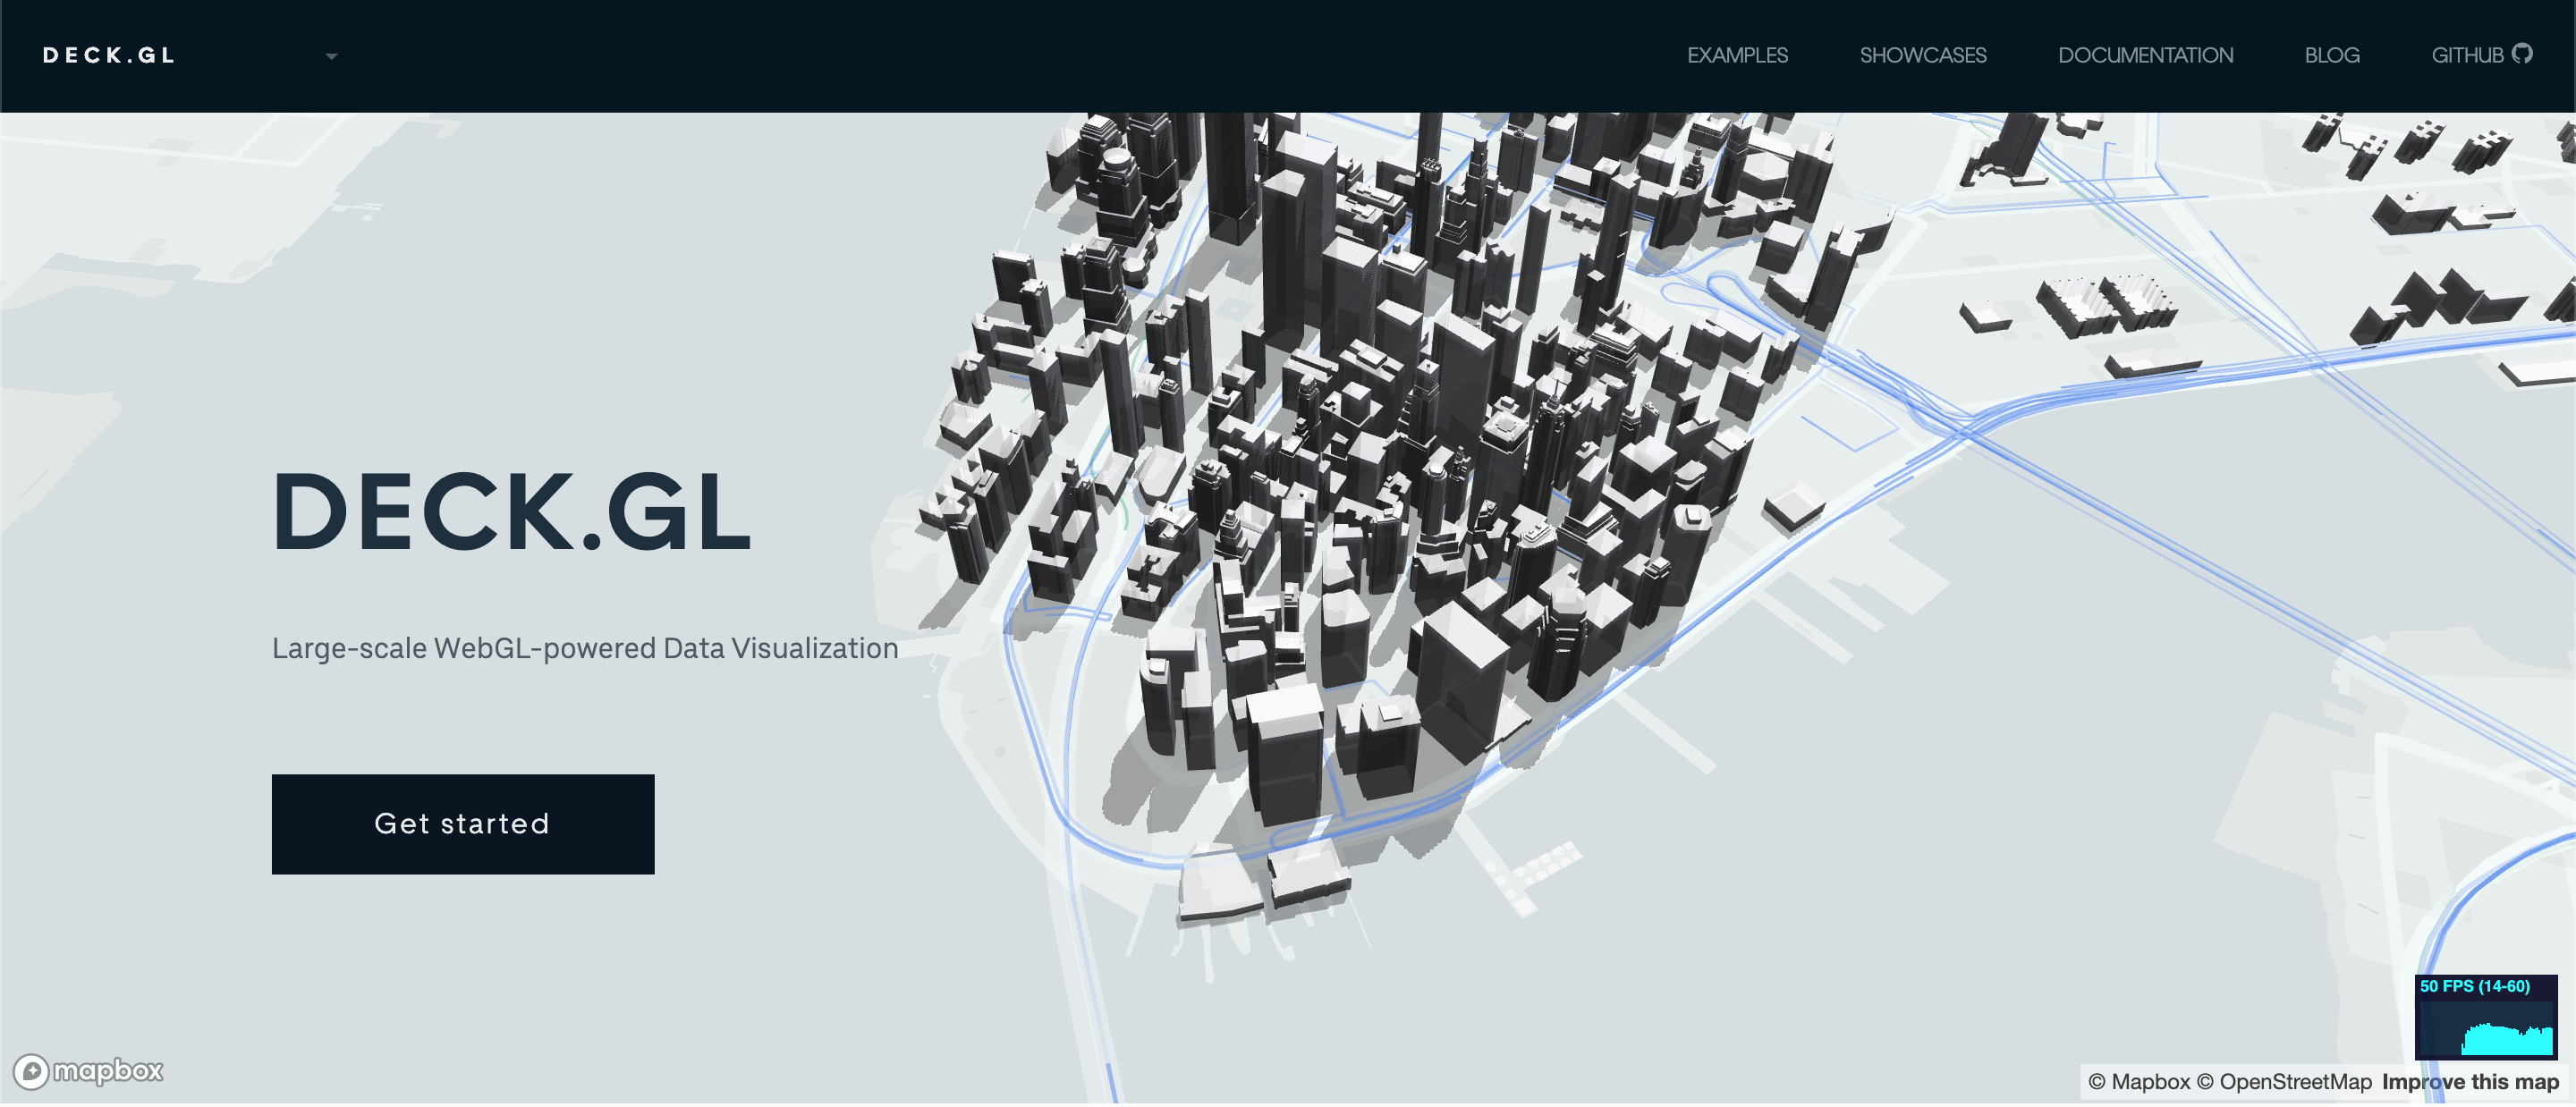
\includegraphics[width=0.9\textwidth]{./Imagenes/UberGL.png}
\caption{\textit{deck.gl}, proyecto de Uber.}
\label{figure:UberGL}
\end{center}
\end{figure}
\newpage
Es en este ámbito en el que aparece la necesidad de una herramienta que sea capaz de 
analizar la información que obtienen los diferentes \ac{GIS}, almacenar y transformar 
este conocimiento para poder generar trayectorias similares a la realidad dentro de un 
territorio geográfico conocido.

\textbf{\textit{track-simulator}} es una \ac{CLI}, propuesta en este documento, para la 
generación de trayectorias pseudo-aleatorias. \textit{track-simulator} cumple una serie 
de requerimientos que están descritos detalladamente en el capítulo 
\ref{chapter:AppArchitecture}. Estos requerimientos son:
\begin{enumerate}

\item Importación de datos en formato \ac{GPX}.

\item Análisis de trayectorias, obteniendo información medible y cuantificable.

\item Almacenamiento de las rutas reales y de los resultados del análisis en base de 
datos

\item Generación de fichero de gráficas resultantes del análisis 

\item Lectura de la base de datos para el acceso a la información

\item Simulación de puntos \ac{GPS}

\item Generación del fichero GPX correspondiente a la simulación de la trayectoria

\item Generación de fichero visualización de trayectoria

\end{enumerate} 

Esta propuesta está desarrollada en el lenguaje Python y utiliza diferentes librerías 
externas, entre las que se destaca \textbf{\textit{osmnx}} para el el análisis a partir del 
uso de redes de caminos y carreteras \cite{Boeing01}, \textbf{\textit{pandas}} para el 
tratamiento de datos \cite{Pandas01} y \textbf{\textit{gpxpy}} para la manipulación de 
ficheros \ac{GPX} \cite{Gpxpy01}. Estas, junto al resto de librerías externas utilizadas 
se describen en detalle en el capítulo \ref{chapter:AppArchitecture}.

La infraestructura de la aplicación está formada a partir de contendores de 
\textbf{Docker} \cite{Docker01}, de esta forma, la aplicación puede ser ejecutada en 
cualquier máquina que tenga Docker instalado, eliminándose cualquier tipo de 
problema que pueda surgir entre dependencias del aplicativo y la máquina en la que se 
ejecuta. Encontramos entonces dos contenedores: el primero contiene una conexión 
con una base de datos MongoDB, en la que almacena tanto las trayectorias analizadas 
como los resultados de los diferentes análisis. El segundo contenedor contiene el 
aplicativo \textit{track-simulator}. Este contenedor contiene todo el código, 
dependencias y configuración necesario para que el usuario pueda analizar un conjunto 
de trayectorias almacenadas en ficheros  \ac{GPX}. Este análisis lo hace a partir de una 
técnica llamada \textit{map-matching} consistente en unir los datos con la red lógica 
de caminos y carreteras.

Después de la etapa de análisis, el usuario puede realizar una generación de 
trayectorias. Estas son generadas de forma pseudo-aleatoria a partir de la información 
analizada en la anterior etapa. Cada trayectoria generada es única en si misma y replica 
el comportamiento de los individuos analizados.

Finalmente como productos resultantes de esta herramienta encontramos ficheros con 
la información resultante del análisis del conjunto de trayectorias, así como ficheros 
\ac{GPX} y representaciones gráficas de las trayectorias simuladas.

Este documento se compone de 8 capítulos donde aparecen 3 diferentes bloques: el 
primer bloque  (capítulo \ref{chapter:PrincipalConcepts} y 
\ref{chapter:AppArchitecture}   serían la introducción al problema y la arquitectura de la 
herramienta. Del capítulo \ref{chapter:DataAnalysis} al \ref{chapter:Experimentation} se 
explican los diferentes módulos que componen el aplicativo y el flujo de los datos, 
explicando detalladamente el análisis de los datos y el algoritmo de simulación de las 
trayectorias, cerrando el bloque con una muestra de los resultados la experimentación 
del aplicativo. Finalmente el capítulo \ref{chapter:GuiaUso} explica al lector como 
instalar y usar la herramienta. El capítulo \ref{chapter:Conclusion} cierra el documento 
con las opiniones finales.

Los capítulos son los siguientes:

\begin{enumerate}[label={C. \arabic*.}]
\setcounter{enumi}{1}
\item \textbf{Conceptos principales}. Capítulo introductorio al lector. Aparecen los 
conceptos básicos y las herramientas conocidas dentro del marco del tratamiento de 
datos \ac{GPS}.

\item \textbf{Arquitectura de la aplicación}. Descripción de las funcionalidades que 
componen la propuesta. Flujo de datos de la herramienta y requerimientos básicos que 
cumple. Se muestra al lector la estructura de \textit{track-simulator} y el problema que 
resuelve.

\item \textbf{Análisis de los datos \ac{GPS}}. Capítulo donde se explica detalladamente 
como se analiza el dato. Desde la preparación del entorno hasta la explotación del dato, 
pasando detalladamente por el proceso de definición de heurísticas y parámetros.


\item \textbf{Simulación de trayectorias}. Explicación del proceso de generación de 
trayectorias pseudo-aleatorias. De define la forma en la que se generan 
individualmente los puntos \ac{GPS}. Se muestra la implementación técnica 
destacable.

\item \textbf{Experimentación}. Muestra de resultados del uso de la herramienta. Se 
realizan dos experimentaciones: con introducción de datos analizados y sin 
introducción de datos. Se muestran gráficas comparativas y se comentan en detalle los 
resultados.

\item \textbf{Guía de instalación y uso}. Conjunto de pasos a seguir para instalar el 
aplicativo en una máquina. En ese capítulo se explican instrucciones disponibles y los 
parámetros necesarios para su ejecución, completando con ejemplos.

\item \textbf{Conclusión}. Capítulo de cierre del documento y de la propuesta. Se 
describe el futuro del aplicativo, así como la opinión personal del desarrollo del 
proyecto. Se concluye la propuesta.
\end{enumerate}
%!TeX root=MemoriaTFG.tex

%Introduction to GPS: The Global Positioning System
%OGC® Geography Markup Language (GML) — Extended schemas and encoding rules

\chapter{Conceptos principales}

En este capítulo se realiza una introducción al lector de los conceptos básicos y las 
tecnologías necesarias dentro del marco de la propuesta. Se realiza a los conceptos de sistemas de 
navegación por satélite, qué tipos principales existen, qué tipos de formatos de 
datos que encontramos y las herramientas principales a tener en cuenta para el tratamiento de datos 
geoposicionales.

\section{Sistemas de navegación por satélite} \label{}
Los \ac{GNSS} son mecanismos de detección de coordenadas geográficas formados por una constelación 
de satélites en órbita utilizados para situar elementos en la superficie terrestre. Estos sistemas permiten 
detectar las coordenadas de posición en un tiempo determinado con relativa exactitud en cualquier
punto del planeta, las 24 horas del día y en cualquier situación meteorológica \cite{Garrido-Villen01}.

Destacan entre muchos sistemas operativos en la actualidad los sistemas GALILEO, GLONASS y GPS, de 
origen Europeo, Ruso y Americano respectivamente, siendo este último el que explicaremos con más detalle 
debido a su mayor uso.

El Sistema de Posicionamiento Global, también llamado \ac{GPS} por sus siglas en inglés 
lo forma un mínimo de 24 satélites en órbita que proporcionan información de posicionamiento y tiempo 
accesible para cualquier usuario. El funcionamiento de estos sistemas se basan el cálculo de la 
distancia de un punto de la tierra a tres satélites aplicando conocimientos de "Position resection" 
\cite{Langley01}.
Esta información tiene una precisión de 100 y 156 metros para la componente horizontal y vertical, 
respectivamente al 95$\%$ de probabilidad \cite{ElRabbany01}.

Es el uso de este sistema el que permite detectar, analizar y medir la situación geográfica de un individuo, y 
esta unidad de información es el elemento mínimo de una trayectoria. En los capítulos posteriores se 
describen tanto las herramientas de manipulación de estos datos como los formatos de almacenamiento.

\subsection{GIS} \label{section:GIS}
Los Sistemas de Información Geográfica, \ac{GIS}, son aplicaciones que permiten almacenar, manipular y 
presentar la información geográfica \cite{EPA01}. Estos sistemas son usados en diferentes campos de estudio 
para el análisis y toma de decisiones. Estas herramientas permiten tratar datos relacionados con la posición de un individuo, datos de la vegetación y entorno urbanístico, permitiendo centralizar, integrar y analizar la información geográfica. Entre el gran número de aplicaciones GIS destacan ArcGIS y QGIS, 
siendo la primera software no libre publicado por la empresa Esri y la segunda software libre por la Open 
Source Geospatial Foundation.
\begin{figure}[!htb]
\begin{minipage}{0.48\textwidth}
\centering
\includegraphics[width=0.9\textwidth]{./Imagenes/ArcGIS.png}
\caption{Ejemplo de la aplicacion ArcGis}
\label{figure:ArcGis01}
\end{minipage}\hfill
\begin{minipage}{0.48\textwidth}
\centering
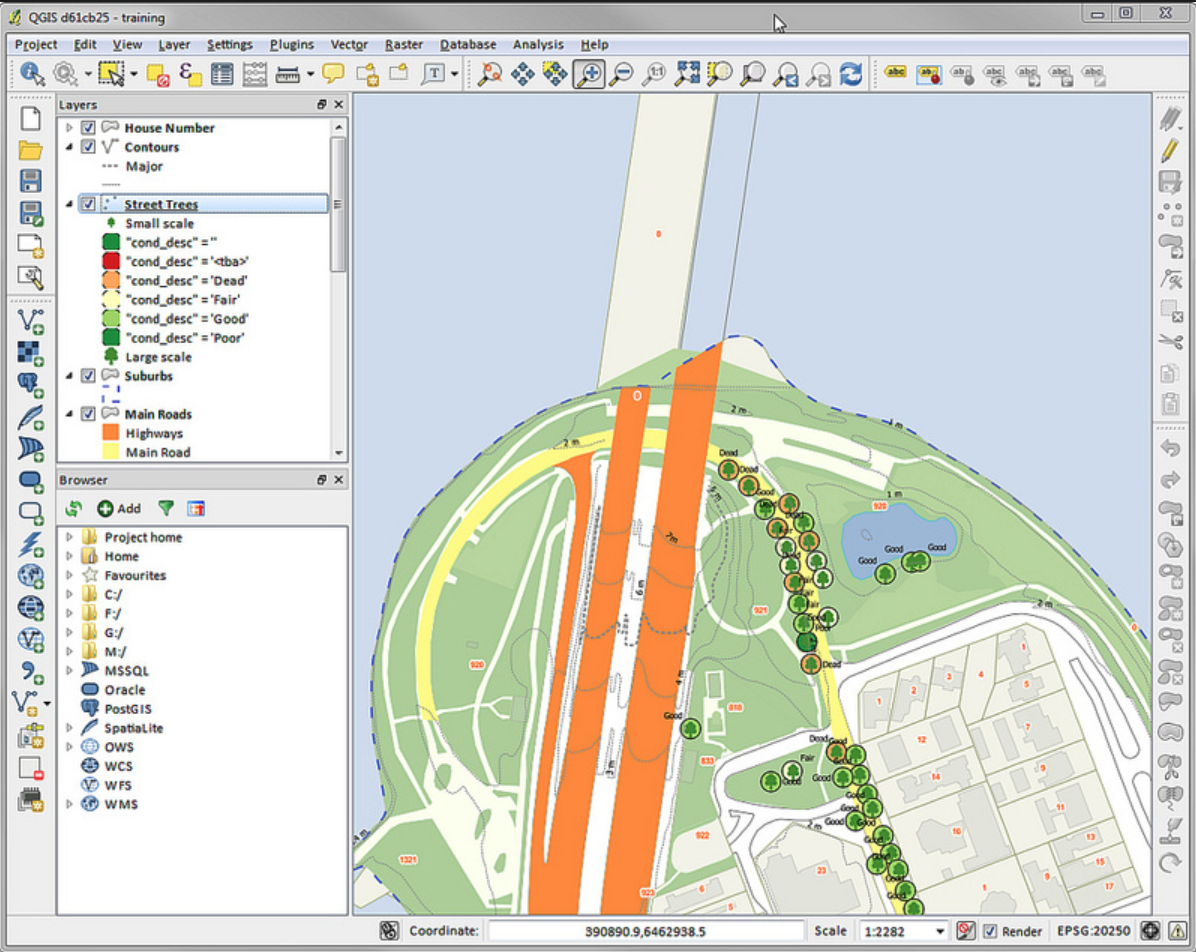
\includegraphics[width=0.9\textwidth]{./Imagenes/QGIS.png}
\caption{Ejemplo de la aplicacion QGIS}
\label{figure:QGIS01}
\end{minipage}
\end{figure}

\subsection{Fuentes de datos}
Las herramientas \ac{GIS} descritas en el apartado \ref{section:GIS} necesitan que los datos obtenidos por los 
los sistemas \ac{GPS} sigan un formato compatible. La información geoposicional es creada y manipulada y 
almacenada en múltiples formatos. Estos se dividen en dos bloques: los formatos ráster y los vectoriales. 

\subsubsection{Formato ráster}
En el formato ráster la representación de los datos se hace a partir de una malla cuadriculada. 
La geografía de un espacio queda descrita en una matriz en la que cada cuadrícula almacena la 
información como altitud o superficie. La gran ventaja que presenta respecto al formato vectorial es que 
la estructura de datos en forma de matriz es simple, no obstante consume más recursos de memoria y la 
resolución de la imagen en los límites entre los píxeles es poco definida si el número de píxeles es insuficiente.
Entre los formatos ráster más populares están Esri Grid, GeoTIFF, JPEG2000 \cite{Morales01}.

\begin{figure}[htb]
\begin{center}
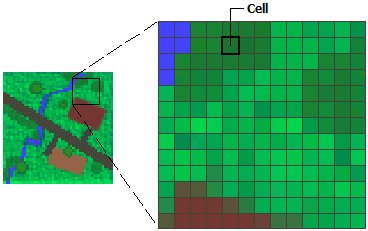
\includegraphics[width=0.6\textwidth]{./Imagenes/RasterImage.png}
\caption{Ejemplo de territorio en formato ráster. \cite{ArgGis01}}
\label{fig:PointGeneration02}
\end{center}
\end{figure}

\subsubsection{Formato vectorial}
Los formatos vectoriales se basan en la representación mediante puntos, líneas y polígonos. Presenta una
arquitectura de datos más compleja que el formato ráster, no obstante es más preciso.
De este segundo grupo destacamos los siguientes:
\begin{description}
\item [\ac{GML}] Lenguaje procedente del esquema \ac{XML} que almacena información geográfica 
\cite{OGC01}.
\item[\ac{KML}] Lenguaje basado en el esquema \ac{XML} para la representar información 
geográfica en un navegador cartográfico como Google Earth o Google Maps \cite{OGC02}.%(KML 2.1 
\item[\ac{GPX}]Formato basado en el esquema \ac{XML} para el intercambio de datos \ac{GPS}. 
En especial para la descripción de points, tracks y routes. La principal ventaja  de este formato 
es la capacidad de intercambio de datos entre diferentes  programas en diferentes entornos 
(Windows, MacOS, Linux, Palm, PocketPC). Es este el formato seleccionado como entrada de datos 
\ac{GPS} del desarrollo de este proyecto \cite{Topografix01}.
\end{description}
Es la flexibilidad de este formato y la representación independiente al tamaño del espacio geográfico 
delimitado las ventajas que determinan su uso en la continuación de la propuesta por delante del formato 
ráster.

Podemos ver en la siguiente figura un ejemplo de  una ruta de una ruta de senderismo por la Serra de 
Tramuntana (Mallorca, Illes Balears, España) en formato vectorial.
\begin{figure}[!htb]
\begin{center}
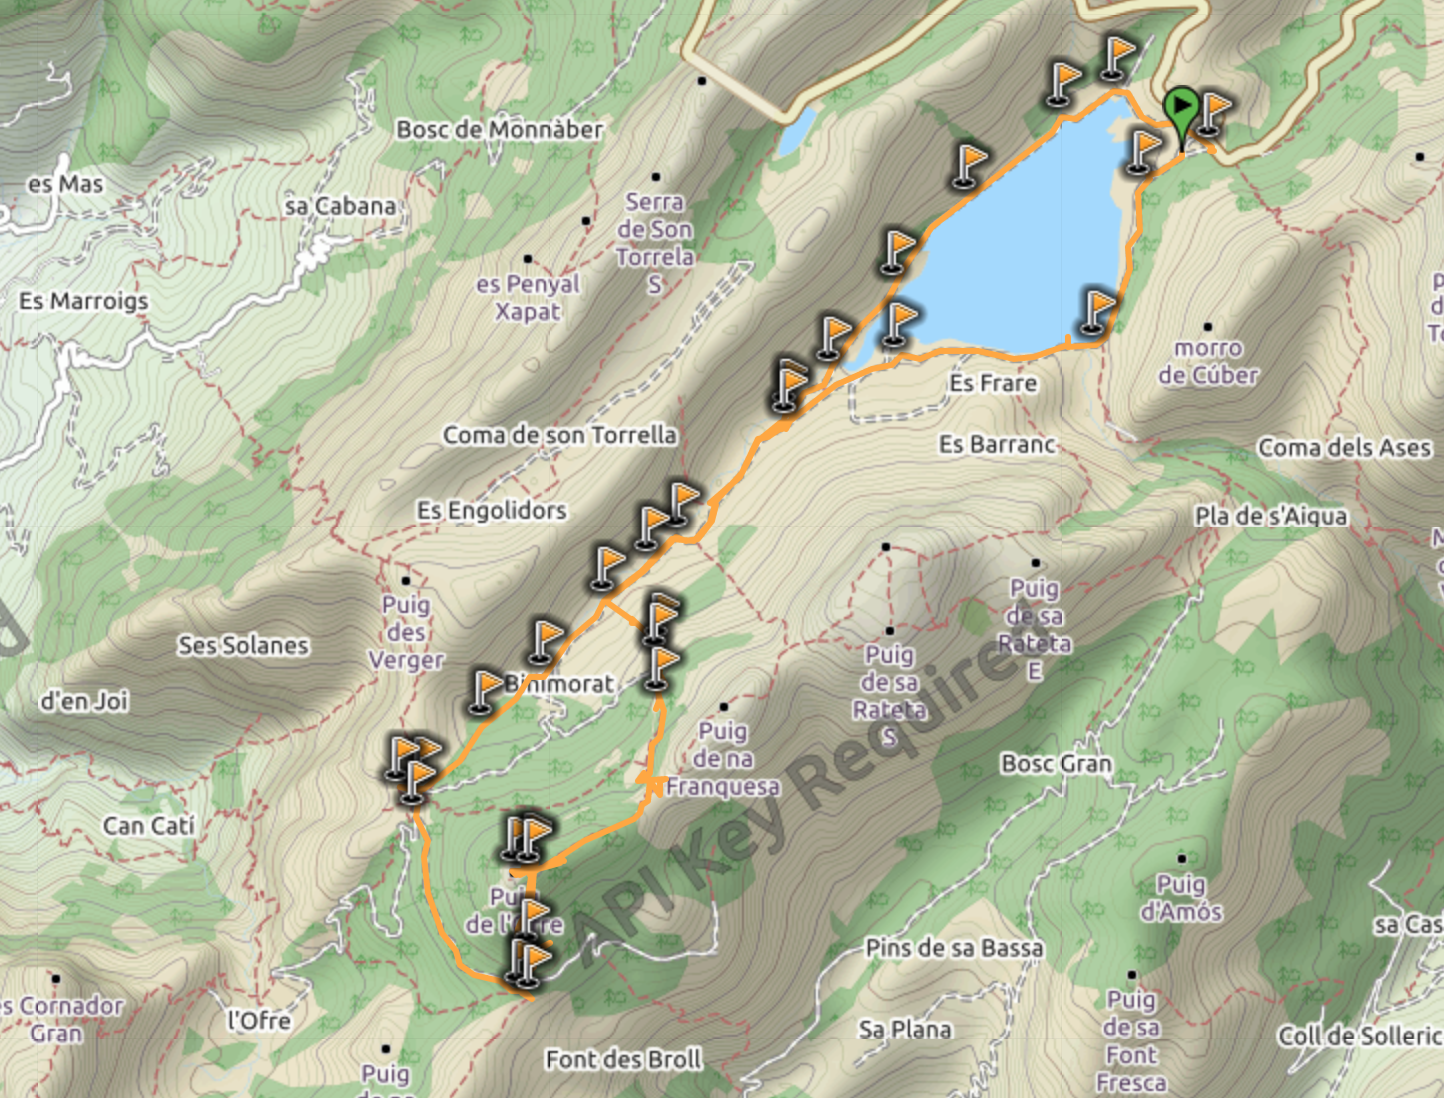
\includegraphics[width=0.5\textwidth]{./Imagenes/RutaOfre.png}
\caption{Ejemplo de Ruta del Puig de l'Ofre, Mallorca, Illes Balears, España.}
\label{figure:PointGeneration02}
\end{center}
\end{figure}
\newpage

\section{Open Street Map}
\ac{OSM} es un mapa interactivo open-source que permite visualizar información geográfica. Las gran ventaja 
de \ac{OSM} es la cantidad de herramientas aportadas por la comunidad que permiten importar, analizar, 
visualizar y editar la información. El formato de fichero \ac{GPX} es el más utilizado dentro de esta 
herramienta. La librería Osmx, que se describe posteriormente hace uso de la información de \ac{OSM} para
importar el modelo de caminos y carreteras necesario para el análisis de trayectorias. Es por lo tanto, la 
plataforma que proporciona el modelo geoespacial lógico en el que se basa la propuesta de este documento.

\section{Estructura de los ficheros \ac{GPX}}
El formato \ac{GPX} al ser basado en \ac{XML} establece sus propias etiquetas y tipos con la información 
del fichero y del espacio geográfico que describe. La etiqueta principal gpx (gpxType) es la raíz del 
fichero \ac{XML}. Presenta de forma obligatoria la versión y el creador del fichero, así como una cabecera 
de metadatos, dónde se describe la información del fichero, autor, así como restricciones de copyright 
de ser necesario. Los elementos esenciales para la descripción de la información geográfica son los 
siguientes:
\begin{description}
\item[\textit{Waypoints} (wptType)] Representación de un punto de interés. Consta de una secuencia de 
elementos 
opcionales para añadir posición, descripción y precisión, así como los atributos obligatorios de latitud/
longitud. Es la unidad mínima de detección de posición geográfica.

\item[\textit{Route} (rteType)] Lista ordenada de Waypoints.  Representan una sucesión de puntos hacia un 
destino. Contiene una secuencia de elementos descriptivos de carácter opcional. No es una representación
de un camino hecho, sino que es la unión de segmentos para llegar de un punto inicial a un punto final. 

\item[\textit{Tracks} (trkType)] Lista ordenada de puntos que escriben un camino realizado. Contiene el 
mismo tipo de secuencia de elementos descriptivos de carácter opcional. La diferencia con una \textit{Route}
es la información que representa. En este caso si que se trata de una detección de un recorrido real.
\end{description}

El formato de una trayectoria en formato \ac{GPX} parte de un \textit{track} inicial, identificado con el tag 
<trk>. El interior está formado por una sucesión de almenos un \textit{segment}, tag <trkseg>, que contienen 
a su vez la unidad mínima, un \textit{point} (<trkpt>). La información que el formato \ac{GPX} permite analizar 
en cada uno de los elementos es diversa. La latitud y la longitud de los elementos \textit{point} es información 
requerida obligatoria para la generación de un fichero \ac{GPX} válido. 
En el algoritmo \ref{algoritmo: fichero GPX} se observa un ejemplo de un fichero \ac{GPX}:

\begin{lstlisting}[caption={Ejemplo fichero GPX \cite{Gpsvisualizer01}} \label{algoritmo: fichero GPX},language=XML] 
<gpx creator="GPS Visualizer https://www.gpsvisualizer.com/" version="1.0">
  <wpt lat="45.44283" lon="-121.72904"><ele>1374</ele><name>Vista Ridge Trailhead</name><sym>Trail 
  Head</sym></wpt>
  <wpt lat="45.41000" lon="-121.71349"><ele>1777</ele><name>Wy'East Basin</name></wpt>
  <wpt lat="45.41124" lon="-121.70404"><ele>1823</ele><name>Dollar Lake</name></wpt>
  <wpt lat="45.39260" lon="-121.69937"><ele>2394</ele><name>Barrett Spur</name><sym>Summit</
 sym></wpt>
  <trk>
    <name>Barrett Spur 1</name>
    <extensions>
      <line xmlns="http://www.topografix.com/GPX/gpx_style/0/2">
        <color>9900ff</color>
      </line>
    </extensions>
    <trkseg>
      <trkpt lat="45.4431641" lon="-121.7295456"></trkpt>
      <trkpt lat="45.4428615" lon="-121.7290800"></trkpt>
      <trkpt lat="45.4425697" lon="-121.7279085"></trkpt>
      <trkpt lat="45.4102075" lon="-121.7140608"></trkpt>
      <trkpt lat="45.4099806" lon="-121.7134527"></trkpt>
    </trkseg>
    <trkseg>
      <trkpt lat="45.4099792" lon="-121.7134610"></trkpt>
      <trkpt lat="45.4091489" lon="-121.7134937"></trkpt>
      <trkpt lat="45.4086133" lon="-121.7132504"></trkpt>
      <trkpt lat="45.4080616" lon="-121.7127670"></trkpt>
      <trkpt lat="45.3928117" lon="-121.6995661"></trkpt>
    </trkseg>
    .
    .
    .
  </trk>

\end{lstlisting}
%!TeX root=MemoriaTFG.tex

\chapter{Arquitectura de la aplicación}

%Qué se puede hacer con TrackSimulator
En esta sección presentamos la arquitectura de la aplicación. Realizaremos una 
descripción de las funcionalidades que presenta y de los módulos de los que consta.

\section{\textit{TrackSimulator}}
\textit{TrackSimulator} es un generador pseudo-aleatorio de trayectorias geoposicionales.

Entendemos como simulación al proceso de recrear el comportamiento, en este caso el camino 
de usuarios dentro de un espacio geográfico. Como muestra esencial y discreta del comportamiento de la 
población se usan registros que han sido obtenidos mediante localización \ac{GPS}. En la figura X
se muestra un ejemplo de una detección del recorrido de un individuo.

\begin{figure}[htb]
\begin{center}
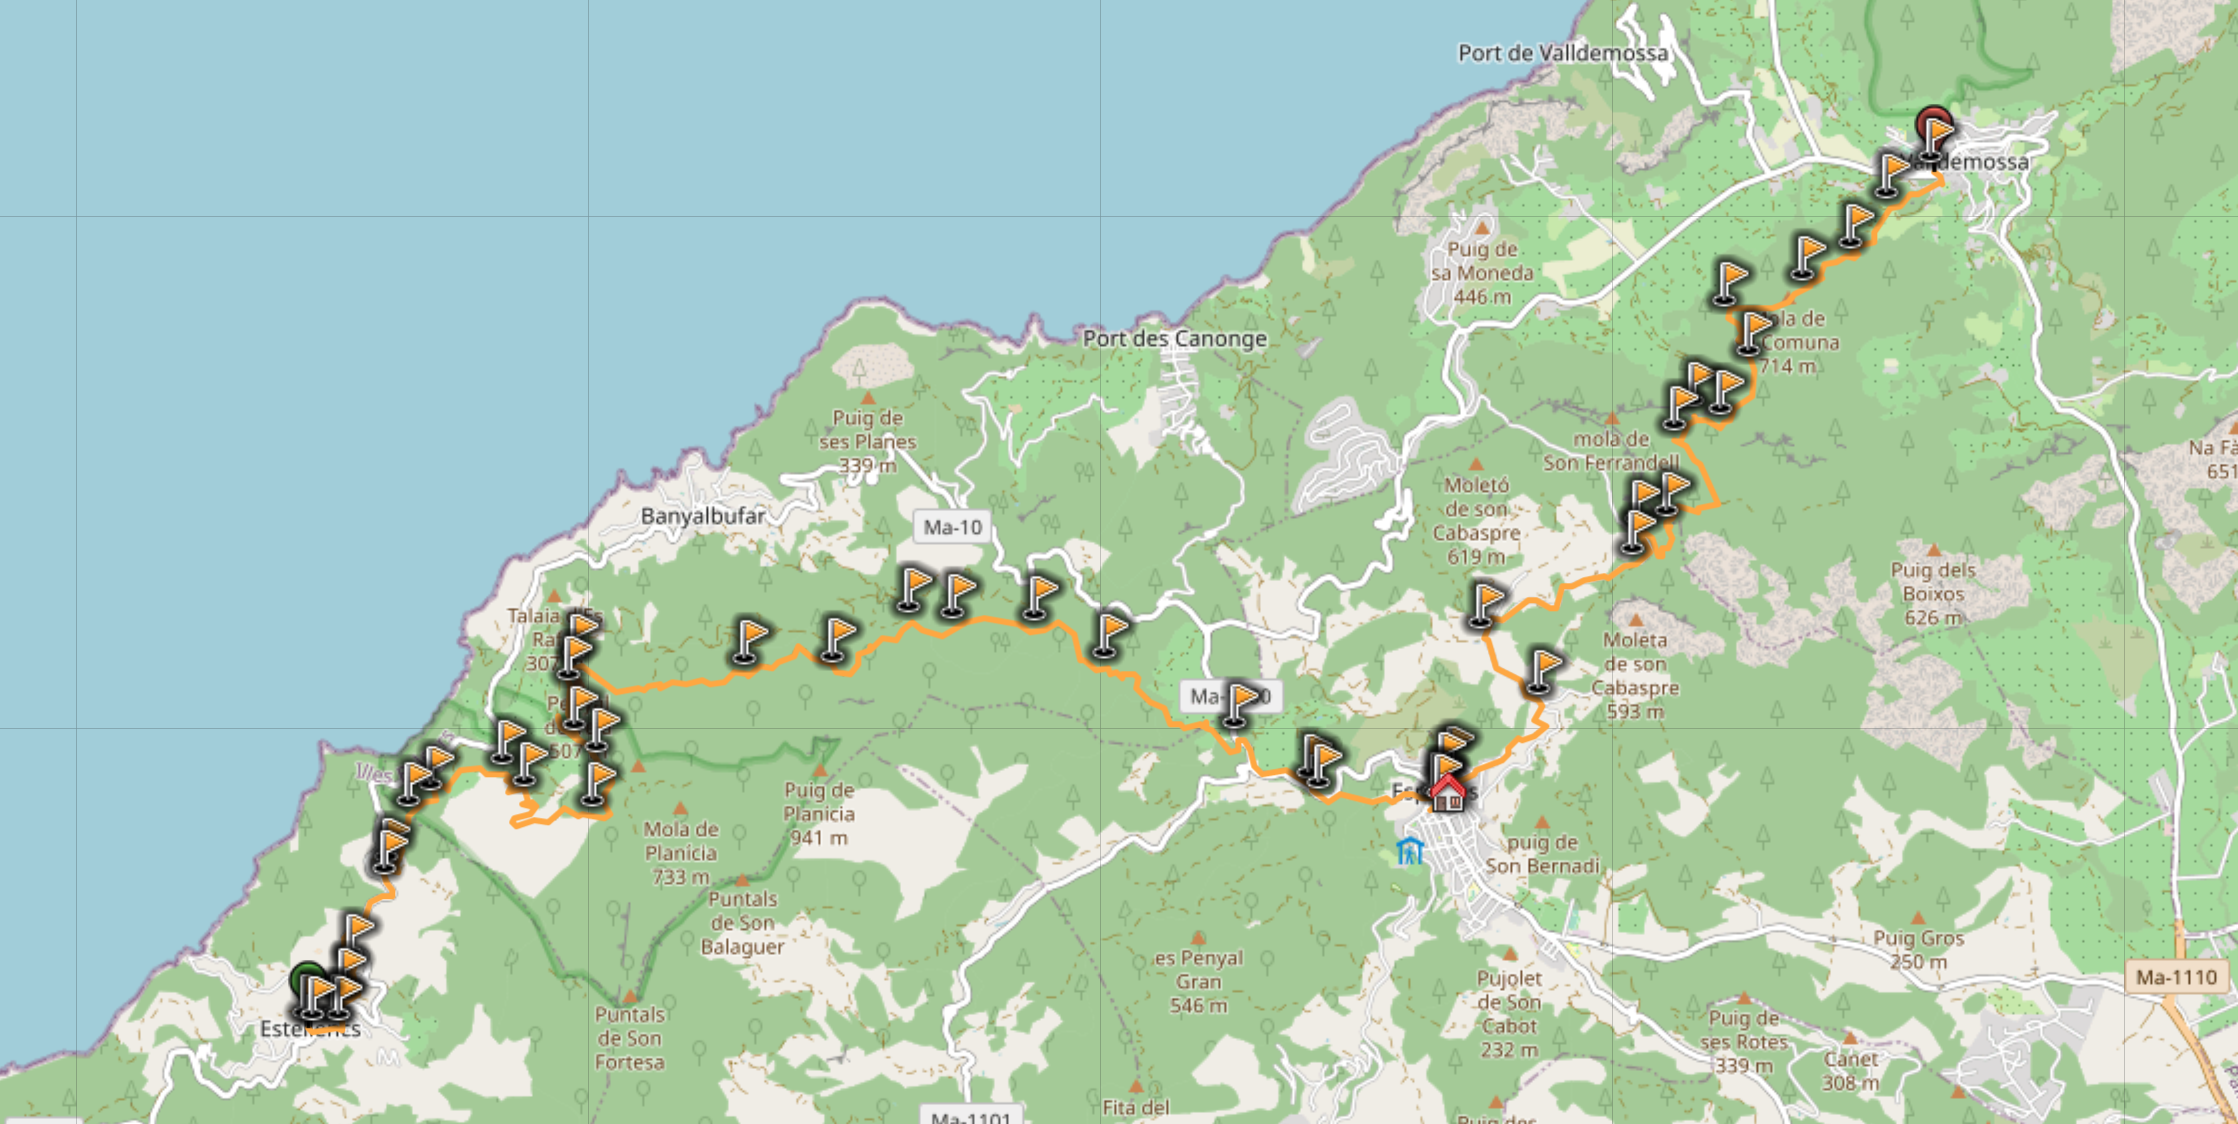
\includegraphics[width=0.6\textwidth]{./Imagenes/RealTrackDetection.png}
\caption{Ejemplo de detección real de la trayectoria de un individuo por la Serra de Tramuntana, Illes 
Balears, Mallorca, Spain}
\label{TrackExample1}
\end{center}
\end{figure}
Para realizar un algoritmo que genere trayectorias y tengan un grado de similitud con la realidad se debe 
realizar un ejercicio previo de análisis y tratamiento de información. Distancias entre las detecciones, 
desviación entre la detección del dispositivo \ac{GPS} y un camino definido son ejemplos de datos que se 
tienen que tener en cuenta para la obtención de resultados óptimos en cuanto a fidelidad a la realidad.

Tanto la información muestral como la generada, así como todo el conjunto de información geoespacial debe 
ser almacenada en un tipo de estructura lógica que permita el acceso y manipulación de estos de la forma 
más eficiente posible. 

Teniendo una estructura lógica que permita almacenar la información, el problema determinante será la 
forma en la que los datos geoposicionales, en este caso puntos \ac{GPS} pasan a formar parte de esté 
modelo. Recordemos que un punto \ac{GPS} contiene únicamente información de la posición dentro de la
superficie terrestre, no obstante no aporta información de la asignación de este punto a un segmento de
un camino, calle, o paraje concreto. Este problema tiene el nombre de \textit{Map matching} y la propuesta
de este documento a su resolución se realizará en detalle en el apartado \ref{section: MapMatching}.

Con la estructura lógica y la información integrada en ella, el análisis de la información permitirá tomar 
el conjunto de decisiones que permitan maximizar el grado de exactitud de la simulación para, 
posteriormente, realizar el algoritmo que permita realizar dicha recreación.

\begin{figure}[H]
\begin{center}
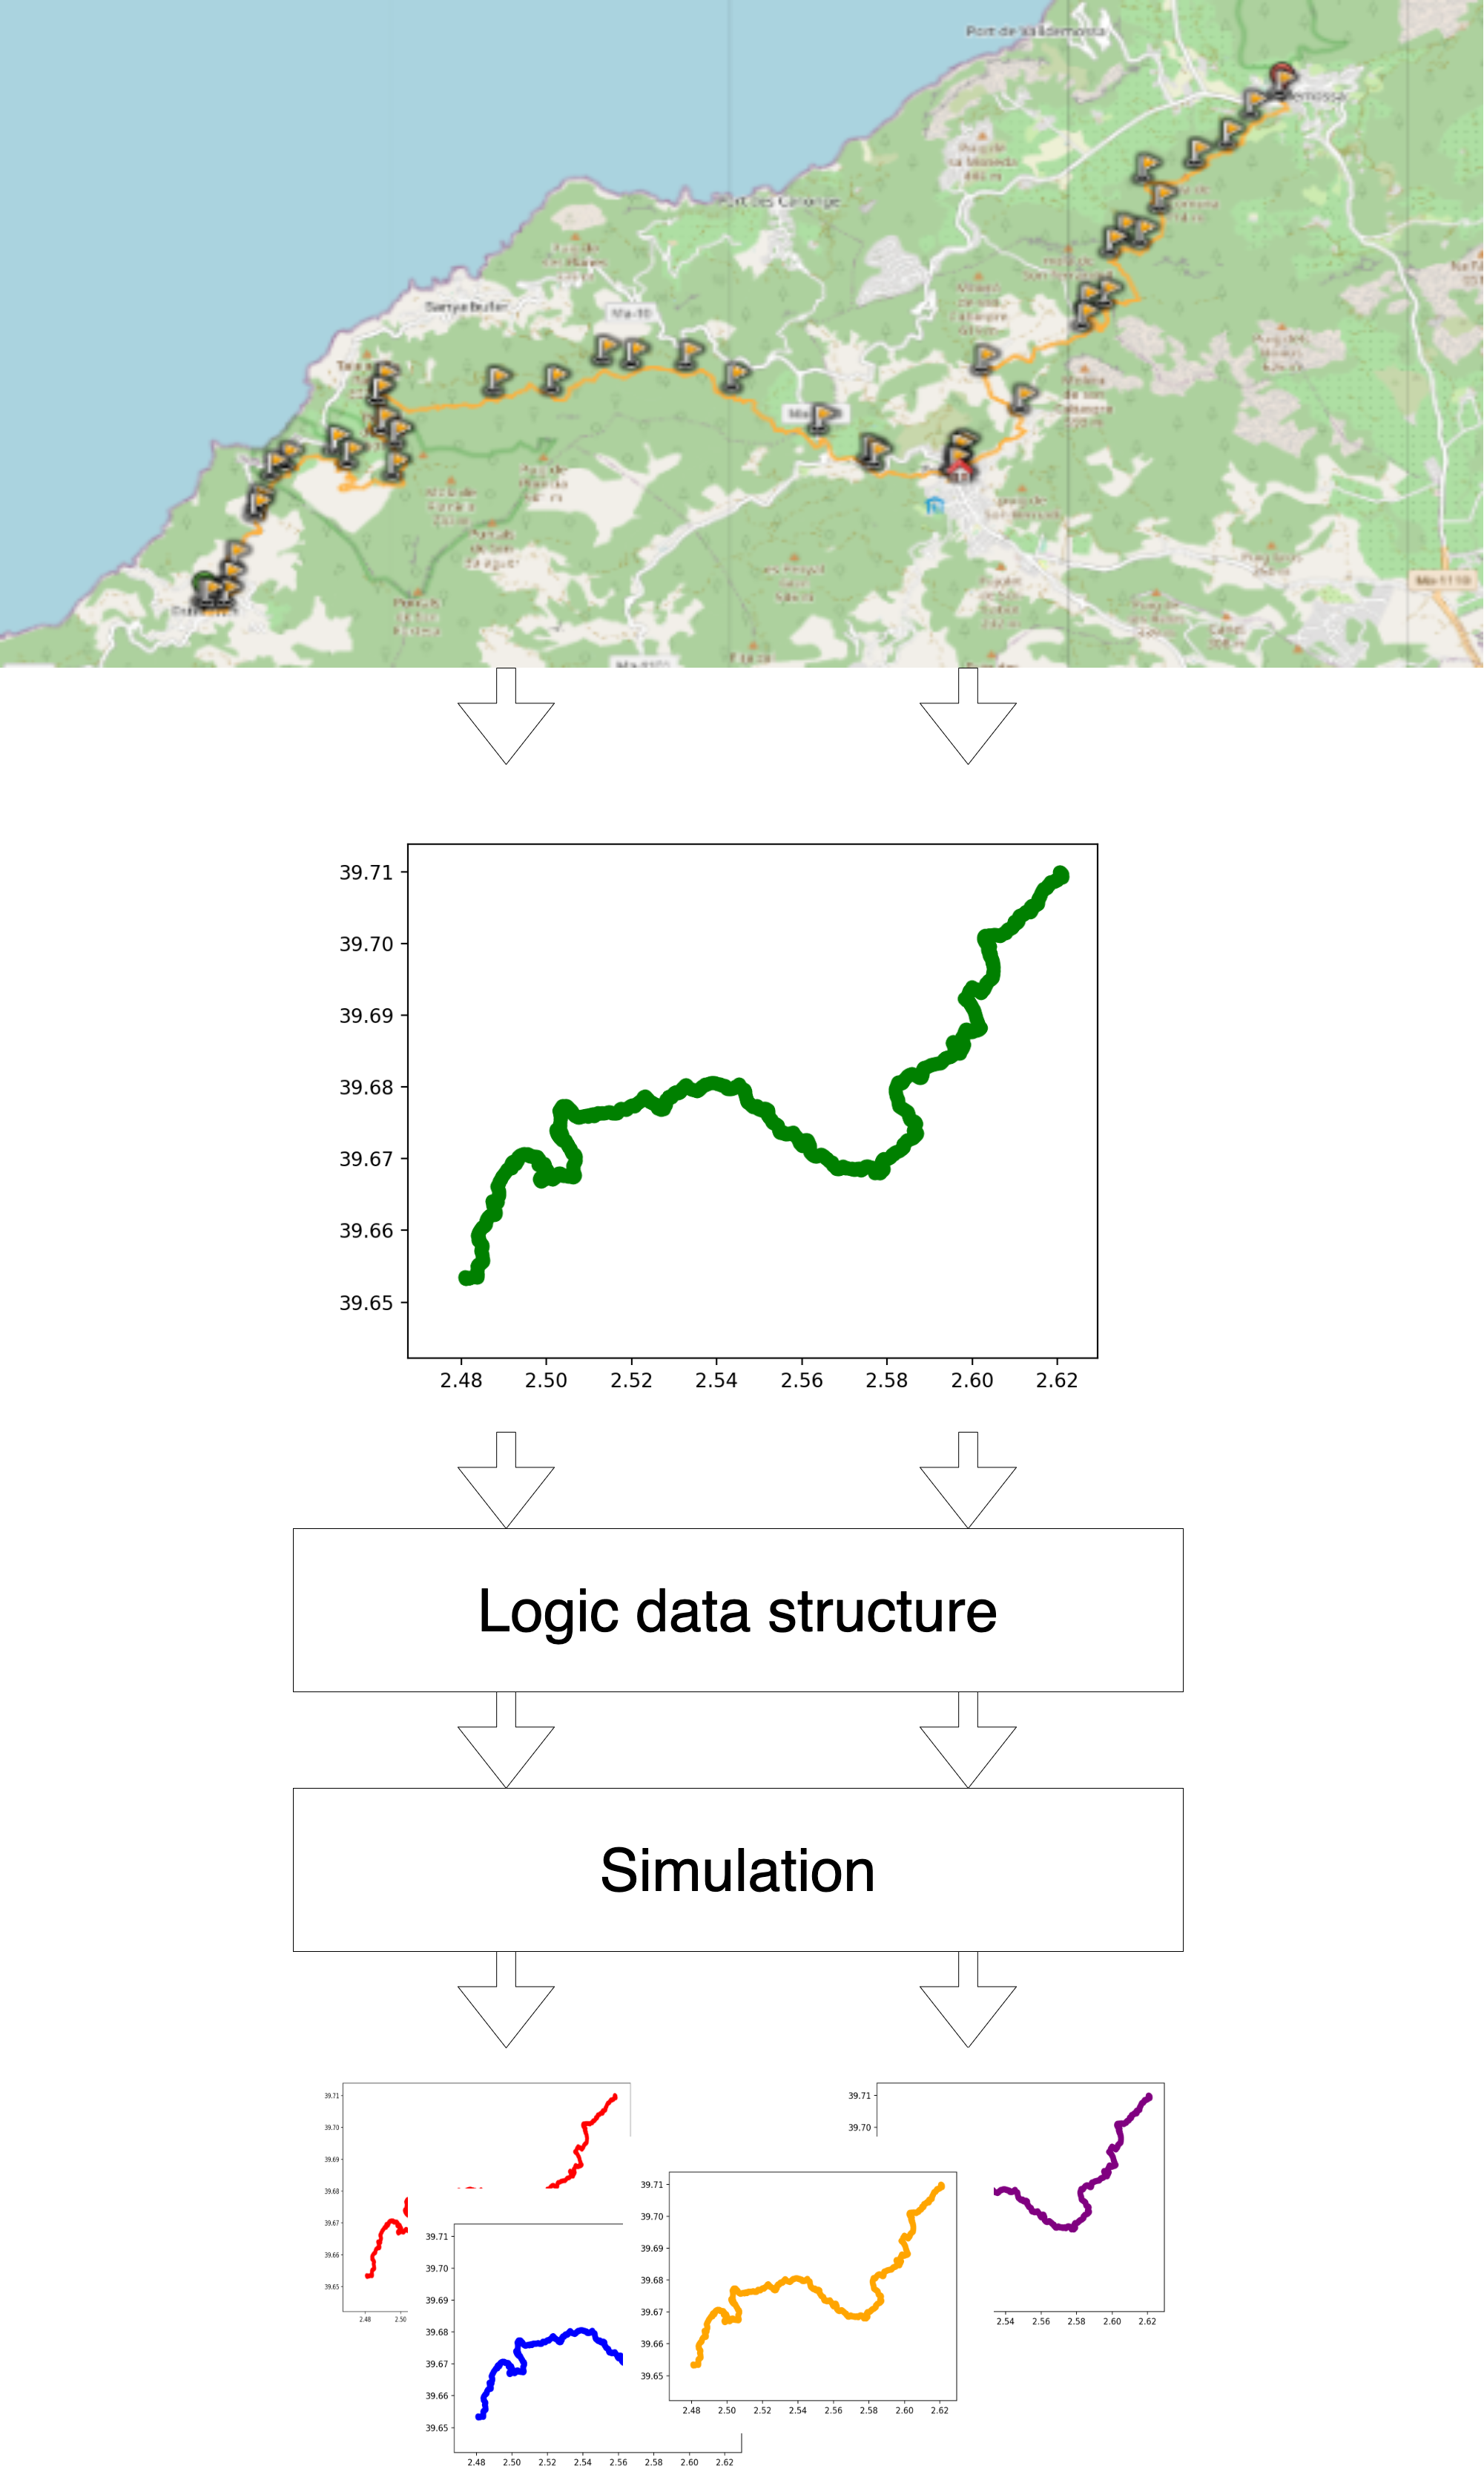
\includegraphics[width=0.5\textwidth]{./Imagenes/TrackSimulatorStructure.png}
\caption{Diagrama de funcionamiento de TrackSimulator}
\label{TrackSimulatorDiagram}
\end{center}
\end{figure}
 
La aplicación crea una sucesión de puntos que equivalen a un recorrido dentro de un plano geográfico. 
Se ha determinado que la aplicación realiza la generación de forma pseudo-aleatoria debido a que 
la producción de los diferentes puntos no sigue ningún patrón o regularidad.

La sucesión de puntos estará relacionada directamente con un camino, sendero o recorrido asignado al 
modelo lógico. La simulación tendrá en cuenta la frecuencia de paso relativa por el segmento como parte
del proceso, así como la distancia entre los puntos.


\section{Funcionalidades de \textit{TrackSimulator}}
\textit{TrackSimulator} es una aplicación. El término \textit{aplicación} se entiende como la suma de 
conjunto de implementaciones  de código, ejecutable y del que se espera un resultado. La aplicación 
permite:
\begin{description}
\item [Importación y análisis de archivos \ac{GPX}] La aplicación soportará la importación de un archivo GPX concreto, 
o bien la ruta de una carpeta con diversos archivos GPX. Estos archivos GPX deben contener trayectorias realizadas en 
el espacio delimitado.

La aplicación, con los datos importados por los archivos, permitirá un análisis de trayectorias aplicando técnicas de 
\textit{map-matching}. Del análisis se obtendrá información:
\begin{description} 
\item[Distancia entre puntos] Como la distancia entre las capturas de posición \ac{GPS} en el fichero.
\item[Distancia relativa entre punto de ruta y punto de trayectoria] Como la distancia del punto \ac{GPS} detectado 
de la trayectoria a la punto proyección dentro de la ruta.
\item[Frecuencia de paso por segmento de ruta] Como la frecuencia de paso por el segmento $x_{a}, x_{b}$ relativo 
a todos los segmentos desde $x_{a}$.
\end{description}


Toda esta información quedará almacenada en una base de datos de forma que la información sea accesible para realizar la simulación de la ruta.

\item [Muestra de resultados del análisis] La aplicación permite la impresión por pantalla de información gráfica de los resultados del análisis.
\item [Creación de una trayectoria a partir de parámetros] Con los resultados de la información analizada se puede realizar una simulación de trayectorias dentro del espacio geográfico.
\item [Exportación de trayectorias a fichero \ac{GPX}] La aplicación permite realizar una exportación de las trayectorias simuladas en formato GPX.
\item [Visualización de la trayectoria] La aplicación mostrará una representación gráfica de la trayectoria tanto analizada como simulada dentro del territorio geográfico.

\end{description}
\begin{figure}[htb]
\begin{center}
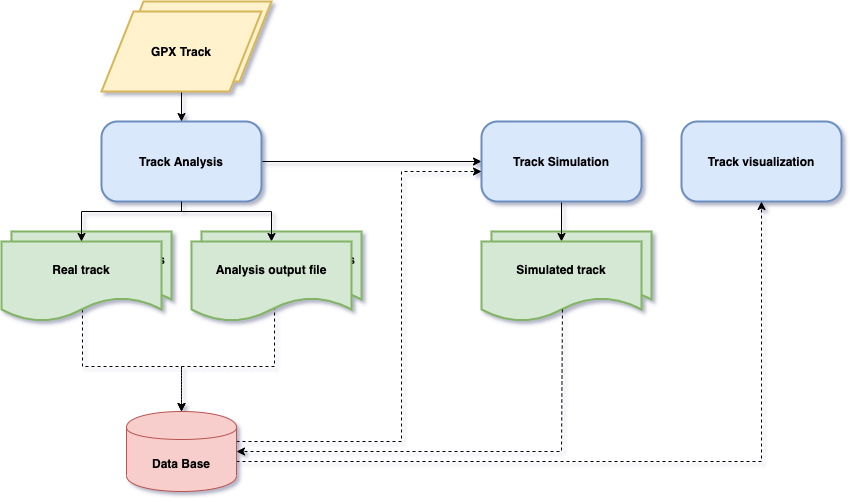
\includegraphics[width=0.9\textwidth]{./Imagenes/TrackSimulatorDiagram.png}
\caption{Diagrama de funcionamiento de TrackSimulator}
\label{TrackSimulatorDiagram}
\end{center}
\end{figure}

\section{Requerimientos de \textit{TrackSimulator}}
\label{section: RequerimientosTrackSimulator}
Explicadas las funcionalidades de la aplicación de Track Analyzer los requerimientos identificados son los siguientes:
\begin{description}
\item[Importación de datos] La aplicación debe realizar una importación de los datos desde un fichero .\ac{GPX} al modelo lógico elegido para la el posterior tratamiento.
\item[Análisis de ruta] La aplicación debe realizar un análisis de la ruta que proporcione por una parte indicadores y por otro valores medibles, cuantificables y utilizables para realizar una simulación 
lo más precisa posible.
\item[Almacenamiento de las rutas reales en base de datos] La aplicación debe realizar un almacenamiento de los datos analizados en una base de datos, con el objetivo de poder ser repetible
sin necesidad de importar nuevamente los datos.
\item[Almacenamiento del análisis en base de datos] La aplicación debe realizar un almacenamiento de los resultados del análisis en una base de datos, con el objetivo de poder ser accesibles para la
etapa de simulación.
\item[Muestra de gráficas del análisis de los datos] La aplicación debe poder realizar una muestra de la información resultante para su visualización por parte del usuario.
\item[Lectura de la base de datos para el acceso a la información] La aplicación debe poder realizar una lectura de la base de datos para acceder a la información necesaria para la muestra de resultados o 
simulación de trayectorias.
\item[Obtención del camino más probable a partir de parámetros de entrada] La aplicación debe poder generar el camino más probable dada un análisis previo y unos parámetros de entrada.
\item[Simulación de puntos \ac{GPS} a partir de resultado de análisis] La aplicación debe generar los puntos de cada uno de los segmentos necesarios dado un camino.
\item[Generación del fichero GPX correspondiente a la simulación de la trayectoria] La aplicación realizar una exportación de los datos a formato .\ac{GPX}.
\item[Visualicación de trayectoria] La aplicación debe poder mostrar al usuario una visualización de la trayectoria dado un fichero .\ac{GPX}.
\end{description}

\section{Implementación de TrackSimulation}
\subsection{Flujo de datos}

\begin{figure}[htb]
\begin{center}
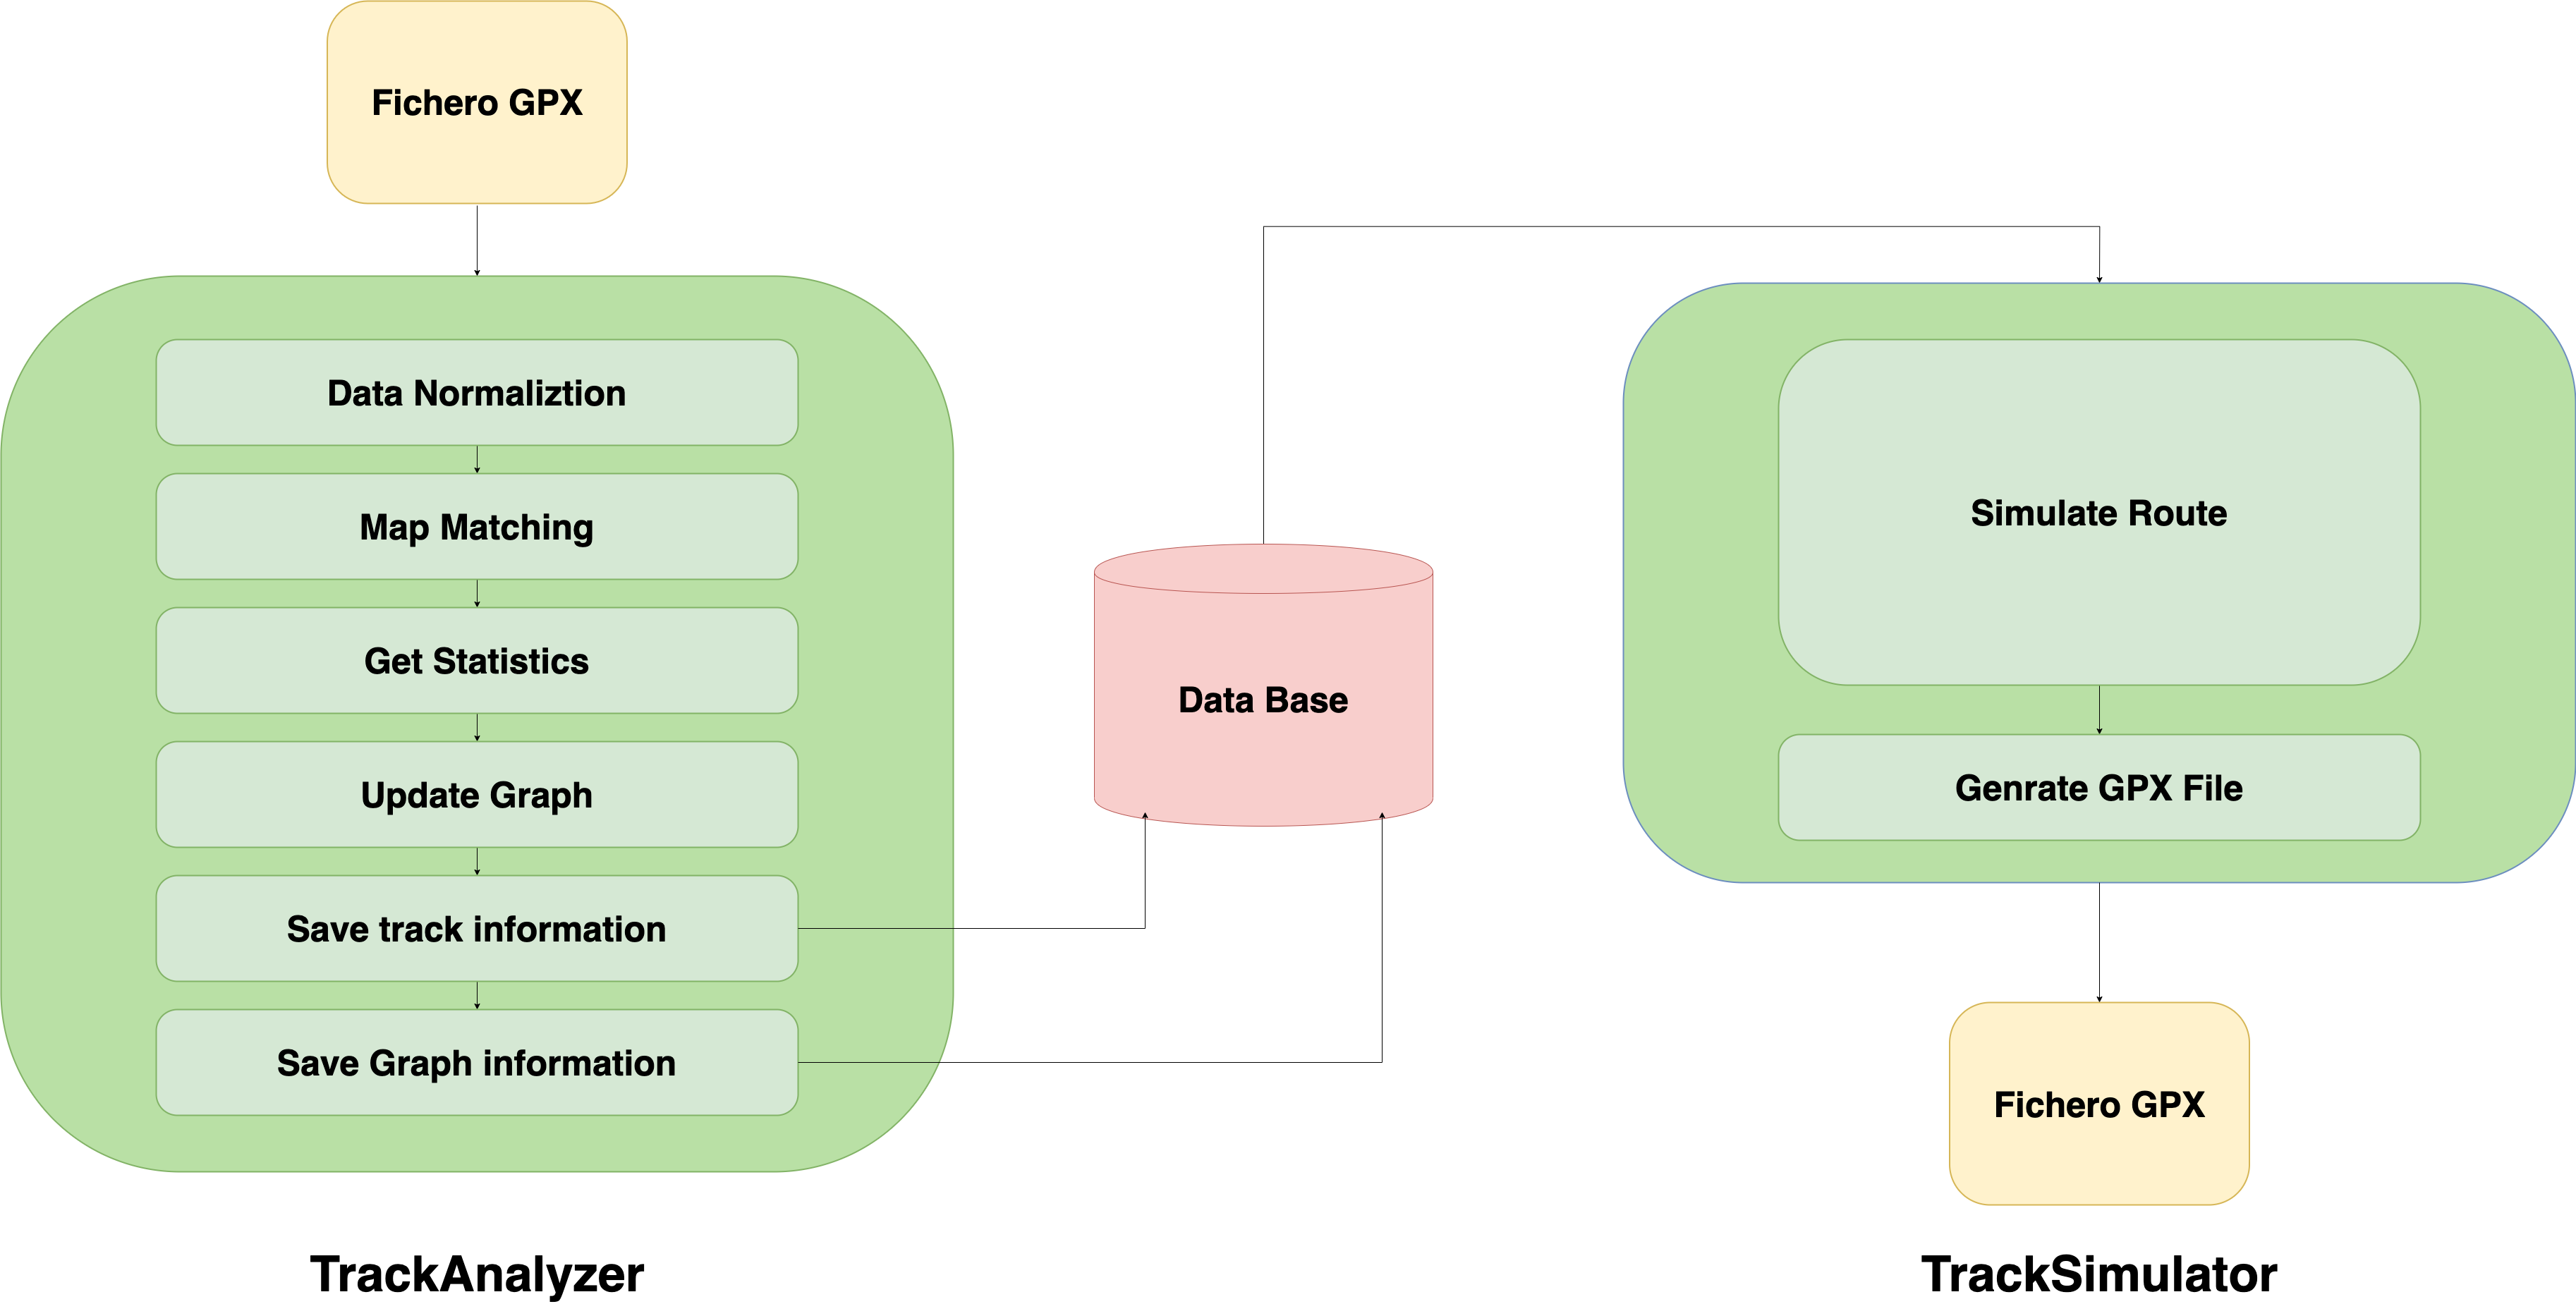
\includegraphics[width=0.9\textwidth]{./Imagenes/TrackSimulatorDataFlow.png}
\caption{Flujo de datos de TrackSimulator}
\label{TrackSimulatorDataFlow}
\end{center}
\end{figure}

Podemos ver en la figura \ref{TrackSimulatorDataFlow} de la parte superior la implementación de la aplicación 
dos grandes módulos. Por una parte encontramos \textit{TrackAnalyzer}. Este módulo es el encargado de 
realizar todas los procesos de tratamiento de datos para su posterior análisis. Inicialmente en el alcance de 
este proyecto se realizará análisis de ficheros \ac{GPX} por lo que es el único modelo de datos que entrará en 
nuestro sistema. Para realizar un análisis se realiza un proceso de tratamiento previo de datos, que se detalla 
en el apartado \ref{section: ImportacionGPX}.

Posterior al tratamiento de datos se realizará el proceso de \textit{Map Matching} con el que se une los datos 
introducidos al modelo lógico del territorio geográfico. El proceso de \textit{Map Matching} queda descrito 
en detalle en el apartado \ref{section: MapMatching}.

Una vez se ha realizado la asignación por cada punto a un camino determinado se puede realizar un análisis 
del fichero, del cual se obtienen las métricas requeridas por el apartado 
\ref{section: RequerimientosTrackSimulator}. La descripción de la forma en la que se explotan los datos está
detallada en la sección \ref{section:ExplotacionDato}.

Con la explotación del dato hecha, únicamente queda guardar la información generada en una base de datos.
El almacenamiento de las trayectorias analizadas y mapeadas, el resultado de los análisis y la estructura 
lógica con la información modificada se realizarán de forma independiente en secciones diferentes de la 
base de datos.

El módulo de \textit{TrackSimulator} tiene la responsabilidad de generar la simulación de una trayectoria 
a partir de unos parámetros de entrada. Una vez generada la simulación, un fichero \ac{GPX} con las 
coordenadas será el producto final del proceso.
 
\subsection{Herramientas externas utilizadas}
Como herramientas externas utilizadas para la realizar la propuesta de este documento se destacan 
el tipo de almacenamiento de datos que se utilizarán, así como las librerías externas que se han usado 
para la implementación de la aplicación. A continuación se detallan ambas.

\subsubsection{Almacenamiento del dato}
Tanto de trayectorias reales como de los datos generados por el análisis deben ser almacenados 
de forma que sean accessibles de forma rápida.
Para el almacenamiento de datos, existen dos grandes posibilidades: El uso de Bases de datos relacionales, 
a partir de ahora descritas como \ac{SQLDB},
o el opuesto, las bases de datos no relacionales, \ac{NOSQLDB}.
Las ventajas de las \ac{NOSQLDB} han hecho que con el paso del tiempo, los desarrollos se vean orientados 
al tipo de almacenamiento no relacional.
Para la realización de la propuesta descrita en este documento se ha decidido realizar el almacenamiento de 
toda la información en \textit{MongoDB}, una de las \ac{NOSQLDB}
más usadas y que detallamos a continuación.

\textit{MongoDB} se trata de una \ac{NOSQLDB} de código abierto y su funcionamiento es documental. 
Se almacenan colecciones de documentos, que son series de elementos JSON clave-valor.

MongoDB elimina las limitaciones de las bases de datos relacionales \cite{Mongo01}. 
Permite almacenar de forma eficiente grandes cantidades de información, siendo
a su vez flexible a modificaciones debido a que los documentos que se almacenan en las colecciones no tienen 
una taxonomía definida. Por lo que el desarrollo incremental de la aplicación y la aparición de nuevos 
campos dentro del modelo de datos no es un problema.
Otro gran motivo para la elección de MongoDB como base de datos de este proyecto es la escalabilidad 
que ofrece, de forma que a grandes cantidades de trayectorias por almacenar, la aplicación respondería 
de forma eficiente y mucho más precisa.

Actualmente para el desarrollo de la propuesta no se ha contado con una gran cantidad de datos.
No obstante el problema ha sido planteado con el objetivo de poder analizar grandes cantidades de datos y que puedan
ser almacenados y accesible mediante el uso de esta base de datos.
\subsubsection{Librerías utilizadas}
Para la realización de las funcionalidades comentadas en la parte anterior se ha hecho uso de las siguientes librerías externas:
\begin{description}
%gpxpy
\item[gpxpy] Librería para la manipulación de ficheros \ac{GPX}. Mediante esta librería se puede realizar una importación del fichero para su posterior manipulación. De esta forma se obtiene la secuencia de puntos \ac{GPS} que describe una trayectoria determinada.
%pandas
\item[pandas] Librería para el análisis de los datos. Toda la información correspondiente a las diferentes trayectorias queda reflejada en un Dataframe para su posterior tratamiento y acceso.
%osmnx
\item[osmnx] Librería para la extracción, visualización y análisis de redes de calles. Mediante esta librería se puede obtener toda la información referente a nuestro espacio determinado del Castillo de Bellver e importar toda la información de sus caminos y carreteras transitables. De esta forma tenemos toda una estructura de datos con información geográfica precisa del entorno. Por otra parte mediante esta librería se puede visualizar las trayectorias escogidas, así como la capacidad de almacenar imágenes de las trayectorias analizadas o simuladas.
%matplotlib
\item[matplotlib] Librería por excelencia para la representación de información de forma visual. Mediante el uso de esta librería podemos mostrar diversas gráficas de la información obtenida y analizada por los diferentes algoritmos.
%numpy
\item[numpy] Librería para el cálculo científico. Esta librería nos aporta diferentes estructuras de datos para el acceso y cálculo de forma eficiente a la información. Una de las principales ventajas de esta librería es la implementación de matrices de forma que el acceso a los datos incrementa su eficiencia de forma considerable.
%geopy
\item[geopy] Librería para el tratamiento de coordenadas. Mediante esta librería se obtienen las herramientas necesarias para tratar al par de datos \textit{(Lat,Long)} como un punto de coordenada  \ac{GPS}. Por otra parte se obtiene implementación del cálculo de la distancia entre dos coordenadas.
%itertools
\item[itertools] Esta librería implementa diversos bloques de iteradores. El uso dentro de nuestro proyecto queda exclusivamente para la agrupación de elementos dentro de un set de datos.
%sklearn
\item[sklearn] Librería para el análisis de de datos. Esta librería nos aporta todas las herramientas necesarias para el análisis de los datos \ac{GPS}. Con ella realizamos los cálculos de puntos próximos a partir de una búsqueda basada en \ac{BSP} como veremos en la siguiente sección.
%shapely
\item[shapely] Librería para el tratamiento de figuras geométricas. De esta forma podemos tratar elementos comos puntos \ac{GPS} de forma abstracta. Por otra parte nos permite tratar las rutas del espacio a analizar como una linea de sucesivos puntos \ac{GPS}.
%pickle
\item[pickle] Librería para la codificación-decodificación de ficheros. Mediante el uso de esta librería se realiza la exportación de la información estadística y de la estructura de grafo generada y almacenada en los ficheros .txt/edgelist sucesivamente.
\end{description}
%!TeX root=MemoriaTFG.tex
\chapter{Análisis de los datos \ac{GPS}} 
\section{Preparación del entorno de datos}
\subsection{Importación de datos GPS a \textit{TrackSimulator}}
\label{section: ImportacionGPX}
%Importación de los datos gpx
Para realizar un tratamiento de los datos a partir de un fichero GPX se realiza un uso de la 
librería \textit{gpxpy}. El primer paso a realizar es el parseo del fichero. De esta forma 
encontramos un objeto track, que contiene segmentos que a su vez contienen los diferentes 
waypoints. De los que hemos hablado anteriormente.
Los waypoints tienen la estructura que podemos ver en esta imagen:

\begin{figure}[htb]
\begin{center}
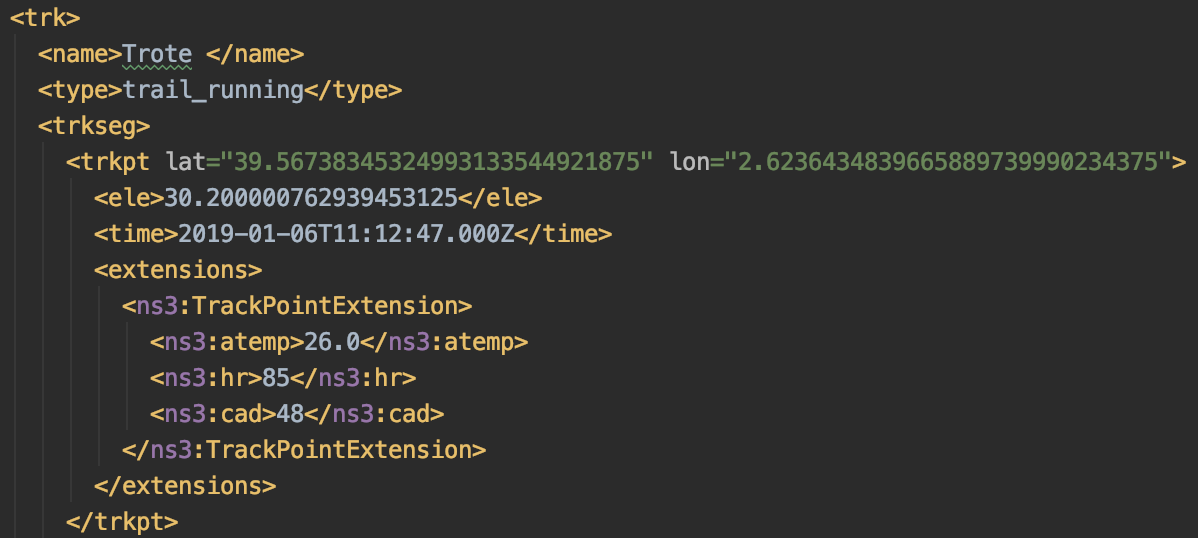
\includegraphics[width=0.9\textwidth]{./Imagenes/WayPointStructure.png}
\caption{Estructura de un \textit{waypoint} dentro de un fichero .\ac{GPX}}
\label{figure: WayPointStructure}
\end{center}
\end{figure}

%Tratamiento de los datos gpx importados

La información necesaria para la implentación de la solución propuesta en este documento es 
la posición en latitud y longitud de cada uno de los puntos. El resto de información no será usada 
para el desarrollo de la propuesta, queda una estructura en forma de lista del siguiente tipo de 
elemento.
\begin{table}[h]
\centering
\begin{tabular}{l | c | l} 
\toprule
\multicolumn{3}{c}{\textbf{Punto preprocesado}} \\ 
\cmidrule(r){1-3}
{\textbf{Campo}} &  {\textbf{Tipo}} & {\textbf{Descripción}} \\
\cmidrule(r){1-3}
{longitud}  & Float & Posición del nodo respecto al eje horizontal. \\
{latitud}  & Float & Posición del nodo respecto al eje vertical.\\
{Point(longitud, latitud)} & Point & Estructura de punto para tratamiento interno. \\
\bottomrule
\end{tabular}
\caption{Estructura lista de puntos.}
\label{TablaNodo}
\end{table}

\subsection{Importación de la red compleja de datos}
\label{section: EstructuraLogica}
%Obtención del grafo
Como apunta G. Boeing en su artículo \cite{Boeing01}  , para abordar correctamente la problemática 
del análisis de rutas dentro del espacio urbano se debe plantear con una solución con una red compleja. 
Esta red está modelada en forma de grafo. Con esta estructura de datos se puede contemplar un proceso 
de importación, análisis, y exportación de datos geográficos. Para realizar la importación de los datos se 
recurre a la librería OSMnx comentada en la sección anterior. Mediante el uso de un corto número 
de instrucciones se consigue importar toda la estructura de la zona del Castell de Bellver.

%Traramiento de la estructura
Con la importación de los datos se ha conseguido obtener la información de OpenStreetMap, 
no obstante se debe realizar un tratamiento de filtrado de los datos importados debido a que aparece 
información que en este proyecto no tienen relevancia. Esta información se trata de características concretas 
de calles, peatonales o no, como la dirección. Nuestro planteamiento del problema define que el la 
trayectoria a simular no tiene en cuenta el sentido de la carretera. Por otra parte, añadiremos información 
tanto a los nodos como a las aristas del grafo para almacenar información necesaria para la solución 
del problema. Por lo tanto al final del tratamiento de la red obtendremos un grafo dirigido, donde las 
intersecciones entre la infraestructura urbana (calle, camino, carretera) está definido como un nodo y 
la característica de esta como la arista. Por simplicidad de entendimiento para la implementación de soluciones 
se ha decididaplicar dos aristas por cada nodo en común, con la información geoespacial correspondiente.
La red compleja queda de la siguiente forma una vez aplicado el procesado:
\begin{table}[h]
\centering
\begin{tabular}{l | c | l} 
\toprule
\multicolumn{3}{c}{\textbf{Nodo}} \\ 
\cmidrule(r){1-3}
{\textbf{Campo}} &  {\textbf{Tipo}} & {\textbf{Descripción}} \\
\cmidrule(r){1-3}
{Identificador}  & Integer  & Clave del nodo.\\
%\cmidrule(r){1-2}
{x}  & Float & Posición del nodo respecto al eje horizontal. \\
{y}  & Float & Posición del nodo respecto al eje vertical.\\
{osmid} & Integer & Identificador de \ac{OSM} \\
\bottomrule
\end{tabular}
\caption{Estructura nodo.}
\label{TablaNodo}
\end{table}
\begin{table}[h]
\centering
\begin{tabular}{l | c | c } 
\toprule
\multicolumn{2}{r}{\textbf{Arista}} \\ 
\cmidrule(r){1-3}
{\textbf{Campo}} &  {\textbf{Tipo}} & {\textbf{Descripción}} \\
\cmidrule(r){1-3}
{Identificador}  & (Integer, Integer, Integer)  & {Clave de la arista}\\
%\cmidrule(r){1-2}
{osmid}  & Integer  & Identificador de \ac{OSM} \\
{oneway} &  Boolean & Carretera de un único sentido. \\
{name} & String & Nombre de la carretera. \\
{highway} & String & Tipo de carretera. \\
{length} & Float & Longitud del camino. \\
{geometry} & LineString & Geometría de la carretera. \\
{num of detections} & Integer & Núm. de detecciones de puntos. \\
{frequency} & Float & Frecuencia de puntos detectados. \\
\bottomrule
\end{tabular}
\caption{Estructura arista.}
\label{TablaArista}
\end{table}

\section{Map Matching}\label{section: MapMatching}
Uno de los grandes retos del análisis de trayectorias es la identificación y asignación de cada uno de los 
puntos GPS en su correspondiente trayectoria. Los puntos GPS se transmiten a partir de un dispositivo. 
Este dispositivo administra la serie de puntos GPS correspondientes a una trayectoria con un cierto error 
y desviación. Esta serie de puntos son puntos aislados y no tienen relación directa con el modelo lógico 
establecido.
Definiremos como \textbf{\textit{Map-matching}} al proceso que nos permite asignar las coordenadas 
GPS a un modelo lógico establecido.
Existen diversos procedimientos para abordar el problema del \textit{Map-matching}. Nuestra 
aproximación al problema la realizamos aplicando el modelo probabilístico de las cadenas de Markov, 
que explicamos en el siguiente apartado.

\subsection{Hidden Markov Model (\ac{HMM})}
%Explicar que es una cardena de Markov
\ac{HMM} sigue el modelo estadístico tradicional de Markov. \cite{Malvar08}. En 1907, A. A. Markov 
comenzó el estudio de un proceso donde un experimento podía afectar a la salida del siguiente 
experimento. Este tipo de proceso se denominó Cadena de Markov. 
%https://www.dartmouth.edu/~chance/teaching_aids/books_articles/probability_book/Chapter11.pdf

Definiremos un conjunto de estados $ S = {s_{1}, s_{2}, . . . , s_{n}}. $ El proceso empieza en un estado 
y se traslada de estado en estado. Esta transición se le denomina \textit{step}. Los \textit{steps} entre 
un estado $S_{i}$  y $S_{j}$ 
cumple una \textbf{probabilidad de transición}.

Por otro lado encontramos la \textbf{probabilidad de emisión}. Esta probabilidad responde a observar 
$o$ en un estado $S$ en un instante $t$ determinado.

Markov define como suposición de primer orden que la probabilidad de ocurrencia de un evento en 
un tiempo $t$ solo dependerá de $t-1$. De esta forma las observaciones ${O-2,..., O-n}$ no 
afectaran directamente a $t$.

%(https://buildmedia.readthedocs.org/media/pdf/hidden-markov/latest/hidden-markov.pdf)
\subsection{Aproximación de Hidden Markov Model a Map-matching}
Nuestra estructura del territorio está definida como un grafo formado por diferentes \textit{nodos} 
y \textit{aristas}. Los nodos corresponden a la intersección entre caminos, mientras que en las aristas 
se almacena la información referente a la constitución geográfica de estos.

Esta información está almacenada en un \textit{Shape} de forma que se trata de una sucesión de puntos 
\ac{GPS} tal 
y como se muestra en la siguiente imagen:
\begin{figure}[htb]
\begin{center}
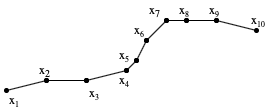
\includegraphics[width=0.6\textwidth]{./Imagenes/LineString.png}
\caption{Ejemplo de estructura LineString}
\label{figure: LineString}
\end{center}
\end{figure}

Cada uno de los posibles puntos de los subsegmentos identificados entre $x_{1}, ..., x_{10}$ son proyecciones 
validas a una observación determinada.

Por otra parte tenemos la información \ac{GPX}. El fichero que almacena la información de trayectorias que 
se han realizado en las delimitaciones de nuestro territorio. Esta serie de puntos se identifican como 
\textbf{observaciones}. Tenemos entonces los dos elementos principales: Una serie de observaciones y 
un modelo. Se plantea el \textbf{problema general de decodificación}: Dada una secuencia de observaciones, 
¿qué secuencia de estados es la más probable para generarlos? Este problema se resuelve mediante la 
implementación del \textbf{\textit{Algoritmo de Viterbi}}, que explicamos a continuación.

%Explicar para que sirve
%Explicar los tipos de cadena de Markov
%Por qué cogemos la Hidden Markov Chain
\subsection{Algoritmo de Viterbi}
El algoritmo de Viterbi se presenta como una técnica computacional con la que se obtiene la sucesión de 
nodos más probable para una cadena de Markov. Para cada una de las proyecciones se obtiene una probabilidad, 
siendo la más alta la elegida para ser el nuevo elemento del camino de Viterbi.

La probabilidad tiene en cuenta dos factores:
\begin{description}
\item [Probabilidad de emisión] Esta probabilidad es calculada por análisis espacial. Por convenio establecemos 
que cuanto más próxima sea la observación a la proyección más probable será que sea la elección correcta, 
partiendo de una distribución normal con media cero tal y como se muestra en la referencia \cite{HMM01}.
\begin{equation}
P_{emission}=\frac{1}{\sqrt{2\pi}\sigma}e^{-\frac{(d_{i}^{j}-\mu)^{2}}{2\sigma^{2}}} 
\end{equation}

\item [Probabilidad de transición] La probabilidad de llegar al estado $S_{i}$ de una proyección viene 
determinado por el estado anterior $S_{i-1}$ en una relación de dos aspectos. Por una parte la distancia 
espacial entre el  $S_{i}$ y $S_{i-1}$ identificado como $d(S_{i},S_{i-1})$. Por otra parte encontramos el 
camino más corto entre estos dos estados. El camino más corto definido como $SP(S_{i},S_{i-1})$ se entiende 
como la cantidad de nodos que se tienen que atravesar para llegar de  $S_{i}$ a $S_{i-1}$. Esta última se mantiene 
como una distribución exponencial de forma que a mayor número de nodos por atravesar en el camino más 
corto esta proyección es penalizada.
\begin{equation} 
P_{transition}=\frac{distance(p_{i-1}, p_{i})}{e^{SP(p_{i-1}, p_{i})}}
\end{equation}
\end{description}

Los valores de $\sigma$ y $\beta$ se han obtenido mediante pruebas. Como vemos en las siguientes figuras,
se han escogido $\sigma = 4$ debido a que es un valor que da unos valores de probabilidad válidos para 
el rango de 5 a 10 metros. 

\begin{figure}[!htb]
\begin{minipage}{0.46\textwidth}
\centering
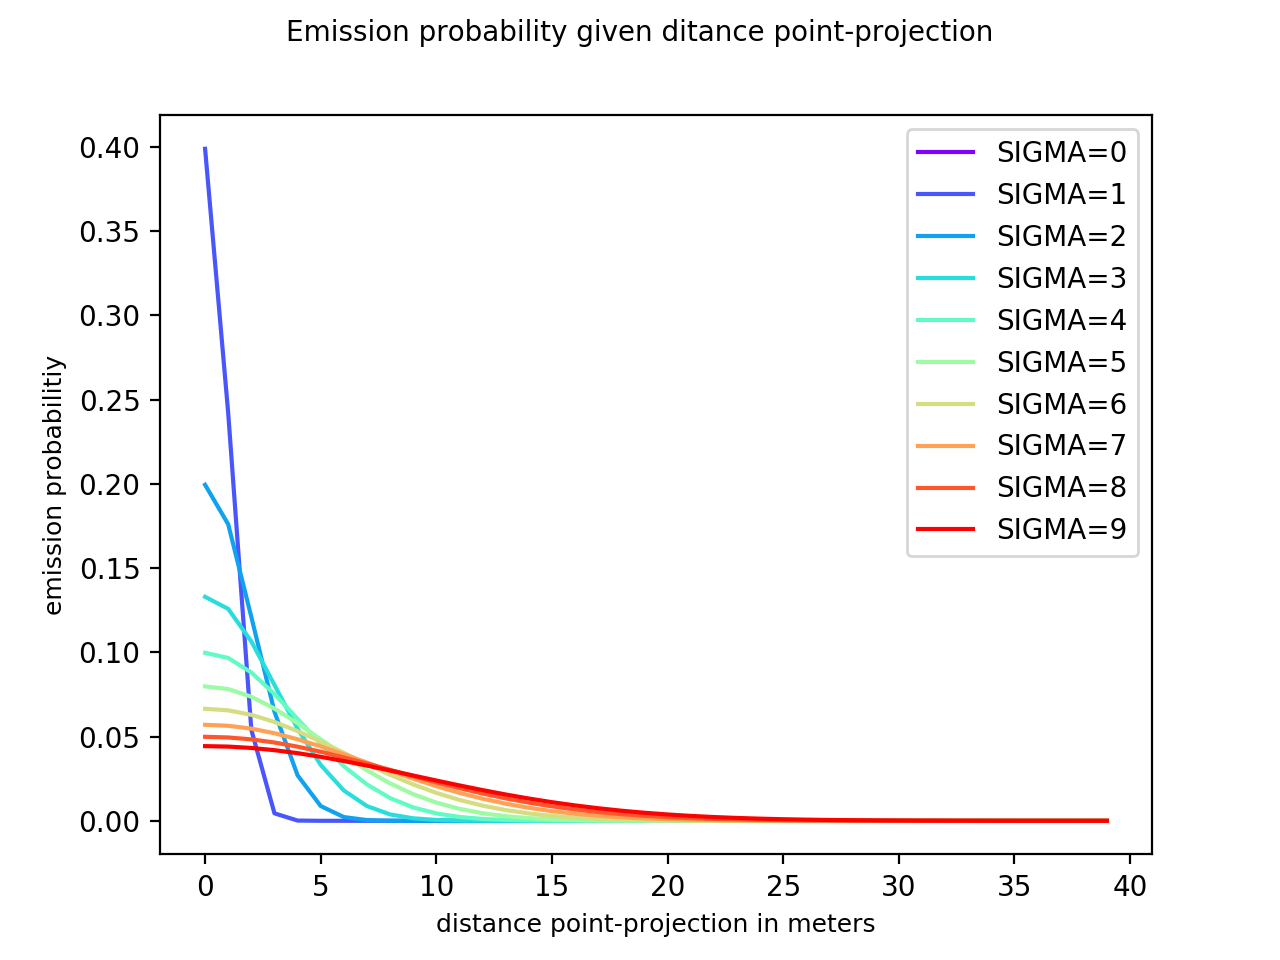
\includegraphics[width=1.2\textwidth]{./Imagenes/EmissionProb.png}
\caption{Análisis de la función de $P_{emission}$ para $\sigma$.}
\label{figure:EmissionProb}
\end{minipage}\hfill
\begin{minipage}{0.46\textwidth}
\centering
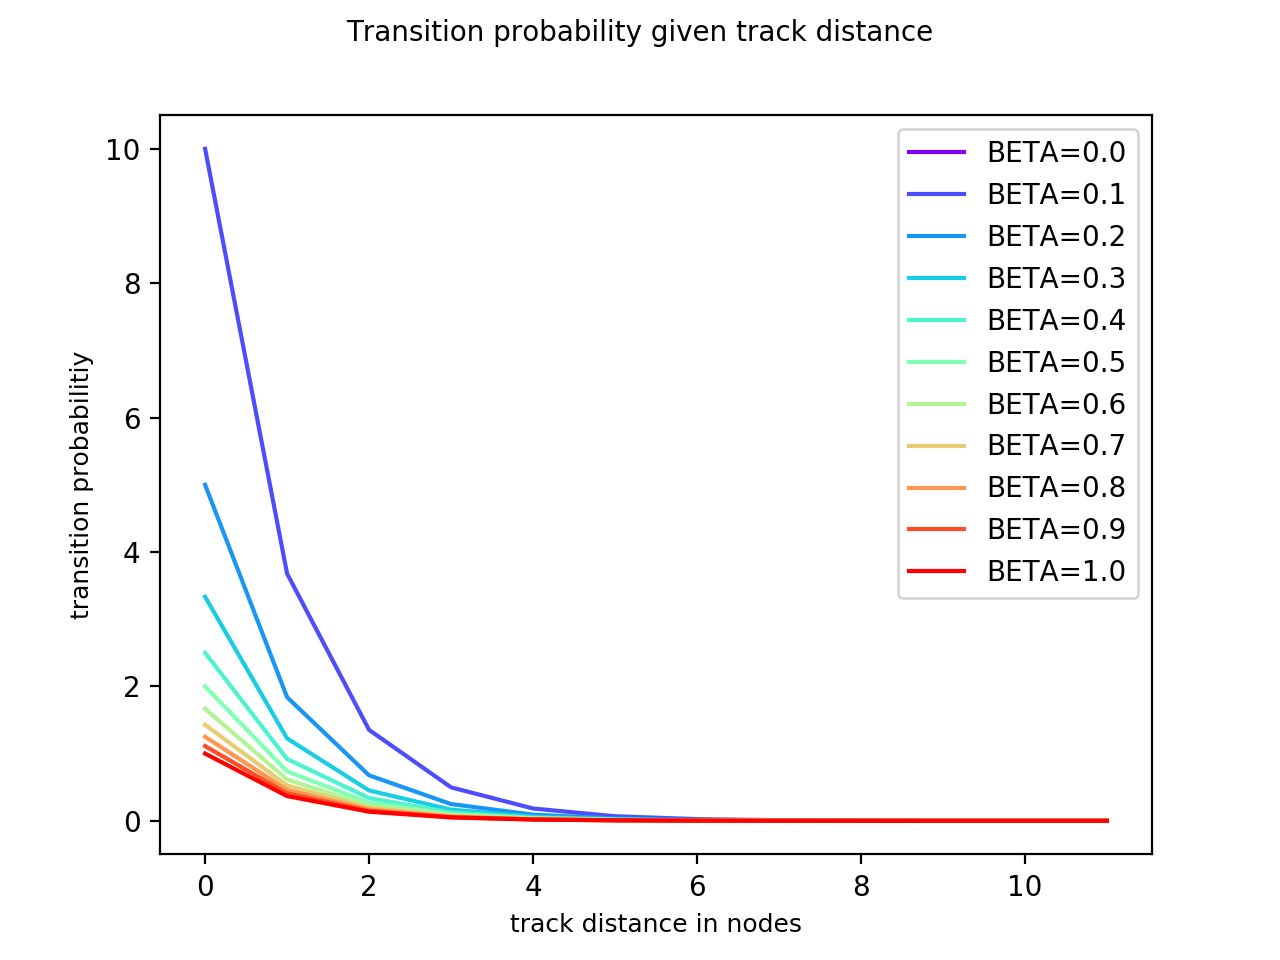
\includegraphics[width=1.2\textwidth]{./Imagenes/TransitionProb.png}
\caption{Análisis de la $P_{transition}$ de transición para $\beta$.}
\label{figure:TransitionProb}
\end{minipage}
\end{figure}
Por otro lado se ha determinado que $\beta = 0.1$ por que la probabilidad de transición 
debido a que es tolerante con valores entre 1 y 3 nodos de distancia, y para los datos tratados ofrece valores válidos.

Cabe destacar que estos valores son modificables según la exactitud con la que cuenten los datos.
%(https://buildmedia.readthedocs.org/media/pdf/hidden-markov/latest/hidden-markov.pdf)

%Implementación propia
La implementación del algoritmo se realiza de forma iterativa para todos los puntos \ac{GPS} de la trayectoria.
Por cada punto se buscarán las proyecciones en un radio determinado. De esta forma se realiza una primera 
criba de proyecciones que no serán probables.
Por cada una de las proyecciones se calculará las probabilidades descritas anteriormente. La probabilidad de 
transición viene determinada por el estado anterior, tal y como se puede observar en la fórmula.
Una vez tratadas todas las proyecciones. Se almacena aquella proyección con la mayor probabilidad total. Si el 
camino más corto entre el nodo correspondiente a la proyección $p_{i}$ y $p_{i-1}$ es mayor que uno se debe 
completar el camino más corto. En la propuesta se tiene en cuenta el posible desfase temporal de los diferentes 
dispositivos localizadores de \ac{GPS}. Si el camino más corto tiene 8 o más nodos se descartará la trayectoria, 
al no ser valorable para el análisis.

Con la aplicación de esta información se obtiene una secuencia de puntos \ac{GPS} relacionados con la estructura de 
datos y queda solucionado el problema del \textit{map-matching}.

\subsection{Ejemplo de aplicación del algoritmo de Viterbi}
Con el siguiente ejemplo se pueden observar los beneficios y los inconvenientes de la aplicación del algoritmo 
implementado en esta propuesta.

En la figura \ref{figure:MapMatching1} se observa en puntos rojos la trayectoria real de un individuo dentro del 
territorio limitado del Castell de Bellver. Los puntos verdes corresponden a la detección de las proyecciones 
más probables por parte del algoritmo de Map-matching.

\begin{figure}[htb]
\begin{center}
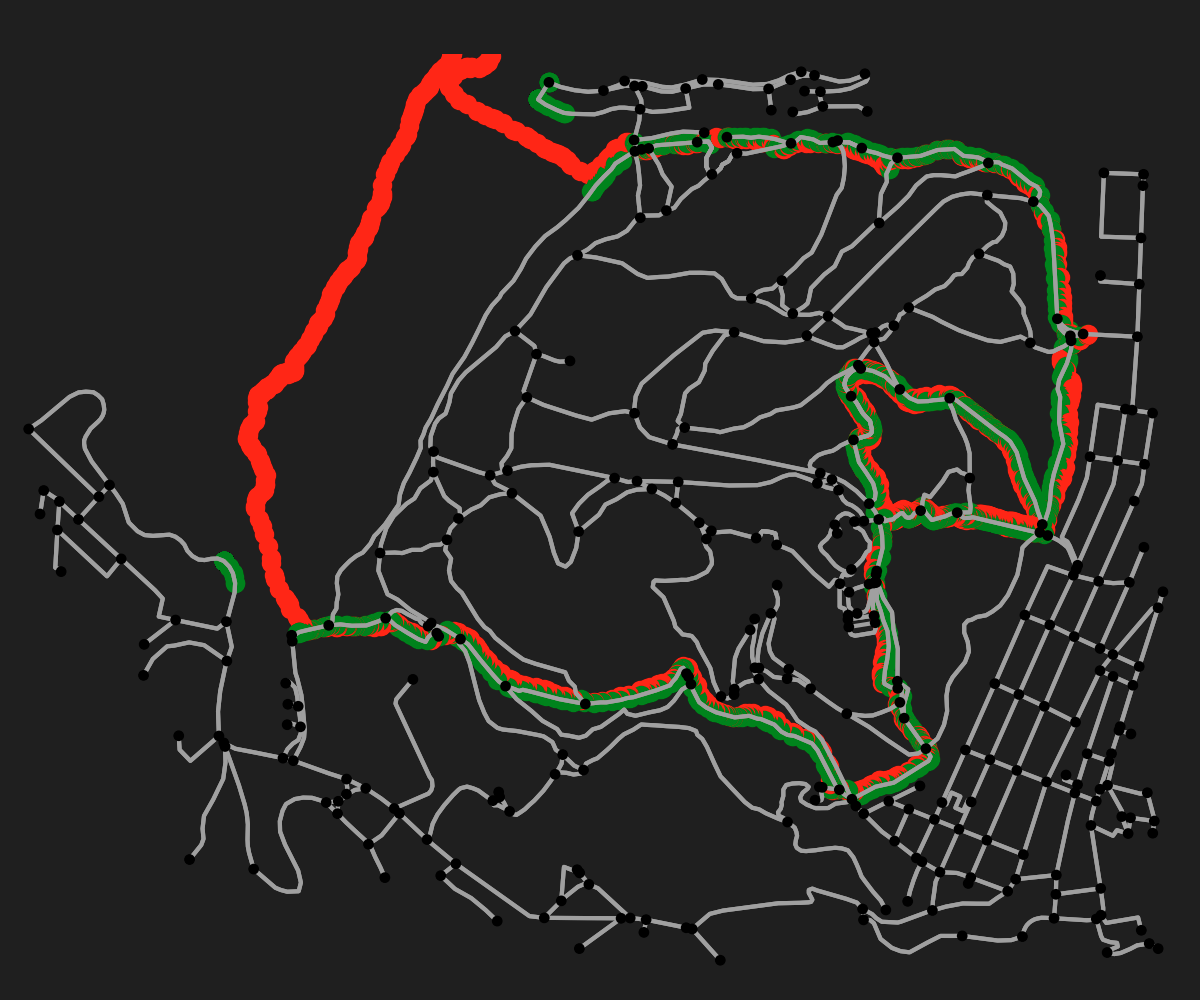
\includegraphics[width=0.6\textwidth]{./Imagenes/MapMatching1.png}
\caption{Ejemplo de aplicación de algortimo de Viterbi para detección de trayectorias.}
\label{figure:MapMatching1}
\end{center}
\end{figure}

El algoritmo realiza una detección punto a punto de su proyección dentro del camino. Pueden 
aparecer situaciones en las que por desviación de precisión en la detección \ac{GPS} un punto parezca 
situarse cerca de un camino no correcto. No obstante, la probabilidad de transición descrita en 
el apartado anterior se encarga de ofrecer como opción más probable, aquella donde el 
\textit{shortest path} del grafo sea menor. \ref{figure:GoodDetection}
\begin{figure}[htb]
\begin{center}
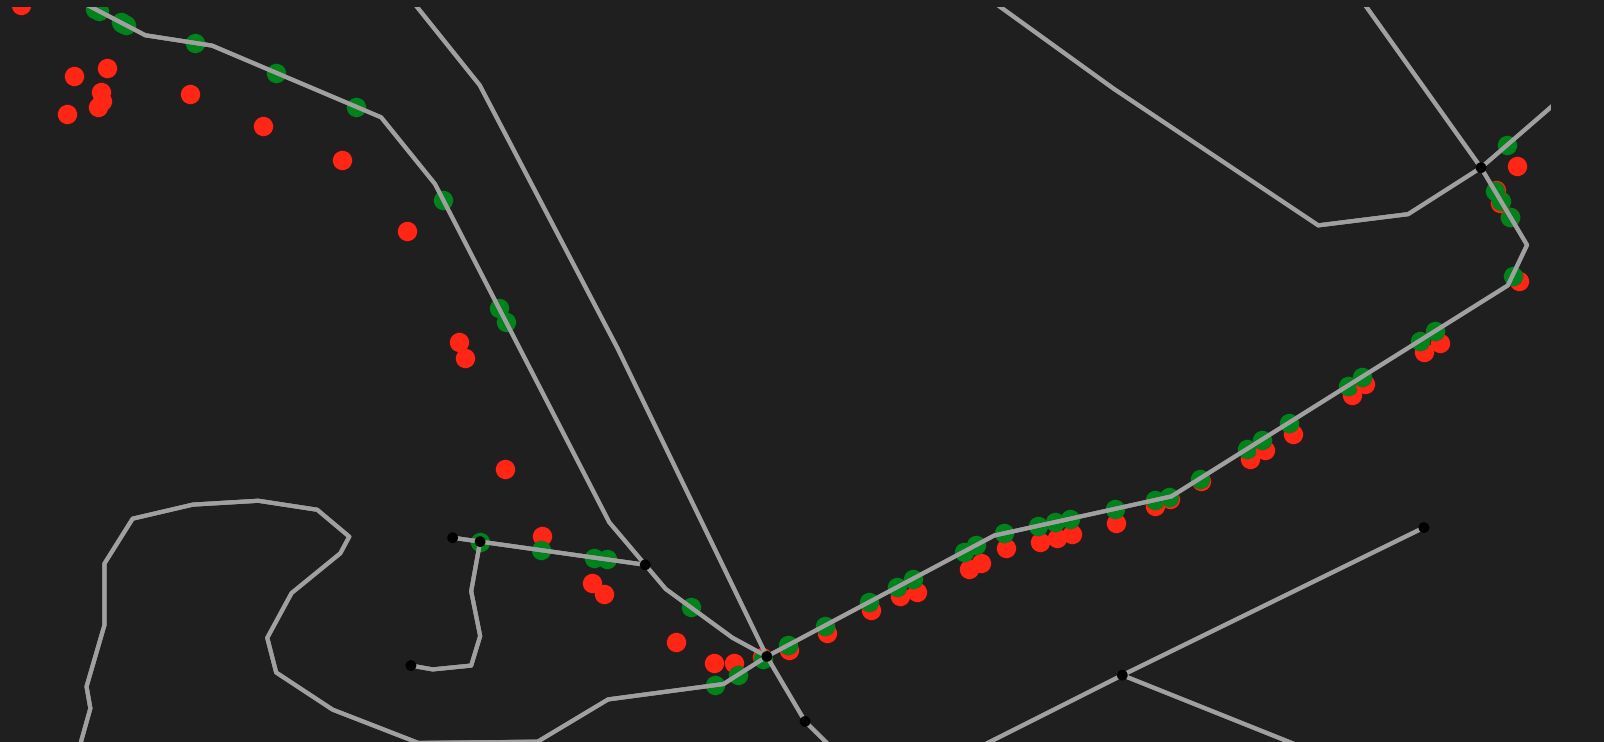
\includegraphics[width=0.6\textwidth]{./Imagenes/BuenaDeteccion.png}
\caption{Ejemplo de aplicación de algortimo de Viterbi para detección de trayectorias.}
\label{figure:GoodDetection}
\end{center}
\end{figure}

No obstante pueden aparecer casos aislados donde la deteccion \ac{GPS} es tan cercana a una 
proyección de un camino incorrecto que hace imposible su no elección respecto a la proyección 
correcta. \ref{figure:BadDetection}
\begin{figure}[htb]
\begin{center}
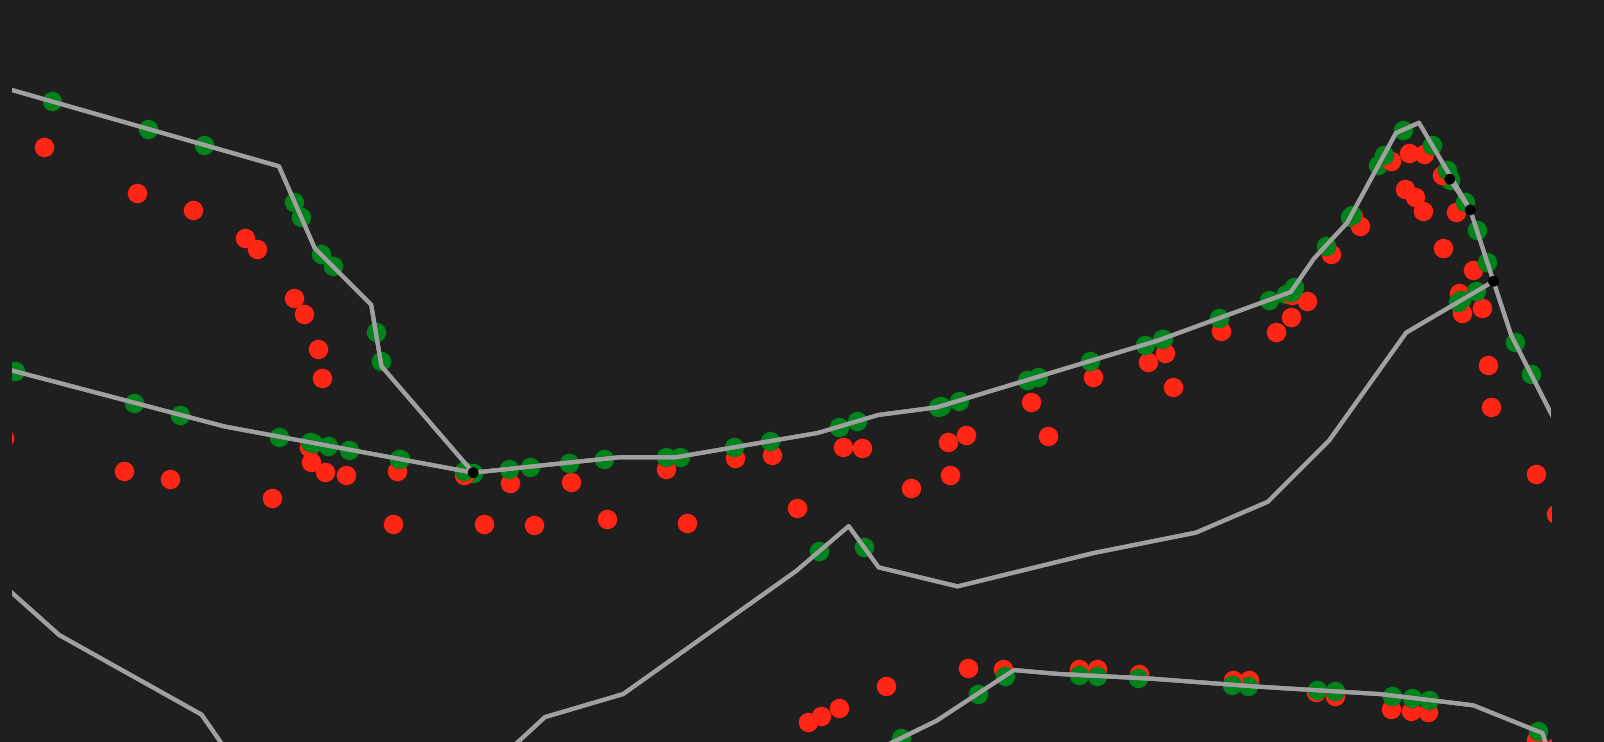
\includegraphics[width=0.6\textwidth]{./Imagenes/MalaDeteccion.png}
\caption{Ejemplo de aplicación de algortimo de Viterbi para detección de trayectorias.}
\label{figure:BadDetection}
\end{center}
\end{figure}

Cabe destacar que el funcionamiento correcto de la detección de proyecciones depende de que el 
individuo realice el recorrido basado en los caminos posibles por el modelo de datos obtenido de \ac{OSM}. 
La detección de puntos por senderos no determinados previamente no pertenece al alcance de este problema.

\clearpage


\subsection{Implementación de Map-matching}
La implementación del algoritmo de map-matching se basa en dos grandes partes: 
el \textbf{\textit{Interactor}} \textit{get\_map\_matching} y la \textbf{\textit{Entity}} 
\textit{hidden\_markov\_model}

\textit{get\_map\_matching} Se trata de una interfaz cuya única responsabilidad consiste en realizar 
el proceso de detección de proyecciones descrito en apartados anteriores. La interfaz se mantiene 
abstracta a la utilización de cualquier otro método que no sea el camino de Viterbi. Es en la implementación 
de esta interfaz (\textit{get\_map\_matching\_impl} la que almacena la lógica. En la implementación propuesta despliega el método \textit{viterbi\_algorithm} de la entidad \textit{hidden\_markov\_model}.

\begin{lstlisting}[caption={Implementación interactor get\_map\_matching\_impl}\label{algoritmo:MapMatchingImpl},language=Python] 
class GetMapMatchingImpl(GetMapMatching):
    def __init__(self, detection_model: HiddenMarkovModel):
        self.detection_model = detection_model

    def match(self, points):
        mapped_track, _ = self.detection_model.viterbi_algorithm(points)
        return mapped_track

\end{lstlisting}

\textit{hidden\_markov\_model} es una entidad abstracta que almacena los métodos necesarios para 
implementar la detección de proyecciones. Los métodos necesarios para implementar una cadena de 
Markov son los cálculos de probabilidad de emisión y de probablidad de transición. Estos junto con la 
implementación del algoritmo de Viterbi describen toda la responsabilidad de esta entidad.

\begin{lstlisting}[caption={Declaración interfaz hidden\_markov\_model}\label{algoritmo:HiddenMarkovModel},language=Python] 
class HiddenMarkovModel(abc.ABC):
    @abc.abstractmethod
    def get_emission_prob(self, projection, point):
        pass

    @abc.abstractmethod
    def get_transition_prob(self, point, projection, next_point, next_projection):
        pass

    @abc.abstractmethod
    def viterbi_algorithm(self, points):
        pass
\end{lstlisting}



\section{Explotación del dato}
\label{section:ExplotacionDato}
Con la problemática descrita en los apartados anteriores resuelta. Tenemos la capacidad de poder inferir 
toda la información  planteada para la propuesta de esta solución.

\subsection{Análisis de distancias}
\label{section: AnalisisDistancias}
La relación $P_{real} - P_{proyectado}$ y $P_{n} - P_{n+1}$, podemos generar la distancia entre estos puntos 
para toda la trayectoria. La distancia que calculamos es la distancia más corta sobre la superficie terrestre, 
la formula elegida es la formula \textbf{Haversine} \cite{Gis01} \cite{Haver01}. Esta fórmula tiene en cuenta 
el radio de la esfera terrestre para realizar el cálculo de la siguiente forma:
\begin{equation}
a = \pi/2 - lat_{1}
\end{equation}
\begin{equation}
b = \cos(lat_{1}) * \cos(lat_{2}) * \cos(lon_{2} - lon_{1})
\end{equation}
\begin{equation}
c = \arccos(a + b)
\end{equation}
\begin{equation}
d = R * c
\end{equation}

Con el cálculo de la distancia encontramos tanto la desviación entre la trayectoria real y la ruta real como 
la distancia entre las muestras de puntos \ac{GPS} de la trayectoria.


La detección de la proyección nos permite saber que caminos se han atravesado para generar la 
trayectoria. Con esta información podemos generar la frecuencia de paso por cada uno de los
caminos. La frecuencia de paso será relativa a la frecuencia de paso de todos los caminos con el mismo 
nodo origen. De esta forma si hay 4 caminos $c_{1,...,4}$ para un nodo $n_{x}$ la probabilidad del punto 
será la siguiente:
\begin{equation}
p_{c_{i}} = \frac{d_{c_{i}}}{\sum{d_{n_{x}}}}
\end{equation}
siendo $d$ el número de detecciones en en la arista.

Esta información será analizada y tratada de forma que el proceso de simulación genere una trayectoria 
basada en información real.La implementación de estos cálculos se realizan en el \textbf{\textit{interactor}}
\textit{get\_analysis\_statistics\_impl}. El método \textit{\_\_add\_next\_point\_distance} y describen la 
comparación de la distancia \textit{Haversine} con el anterior punto, o bien con la proyección.

\begin{lstlisting}[caption={Método add\_next\_point\_distance}\label{algoritmo:addNextPointDistance},language=Python] 
    def __add_next_point_distance(self, data: DataFrame) -> DataFrame:
        data['point_lon_shift'] = data.Point_lon.shift()
        data['point_lat_shift'] = data.Point_lat.shift()
        data['DistanceToNext'] = data.apply(lambda x: Point(x['Point_lon'], x['Point_lat']).haversine_distance(
            Point(x['point_lon_shift'],
                  x['point_lat_shift'])),
                                            axis=1)
        return data.drop(columns=['point_lat_shift', 'point_lon_shift'])
\end{lstlisting}


\begin{lstlisting}[caption={Método add\_point\_projection\_distance}\label{algoritmo:addPointProjectionDistance},language=Python] 
    def __add_point_projection_distance(self, data: DataFrame) -> DataFrame:
        data['DistancePointProjection'] = data.apply(lambda x: Point(x['Point_lon'],
                                                                     x['Point_lat']).haversine_distance(
            Point(x['Projection_lon'],
                  x['Projection_lat'])),
                                                     axis=1)
        return data
\end{lstlisting}


\subsection{Demostración de análisis}
A continuación se mostrarán los resultados de un análisis utilizando la metodología mostrada en 
la parte superior del documento, se cuenta con una muestra de 25 rutas reales realizadas 
recorriendo diversos caminos en el territorio acotado del Castell de Bellver. Destacamos que parte 
de la muestra contiene casuísticas donde el individuo ha realizado recorrido por territorio no identificado 
como ruta. Para sopersar este impacto dentro de los resultados se han \textit{outliers} aquellos puntos 
que superen una distancia superior a 40 metros. El análisis realizado nos deja el siguiente resultado:
\begin{figure}[!htb]
\begin{minipage}{0.48\textwidth}
\centering
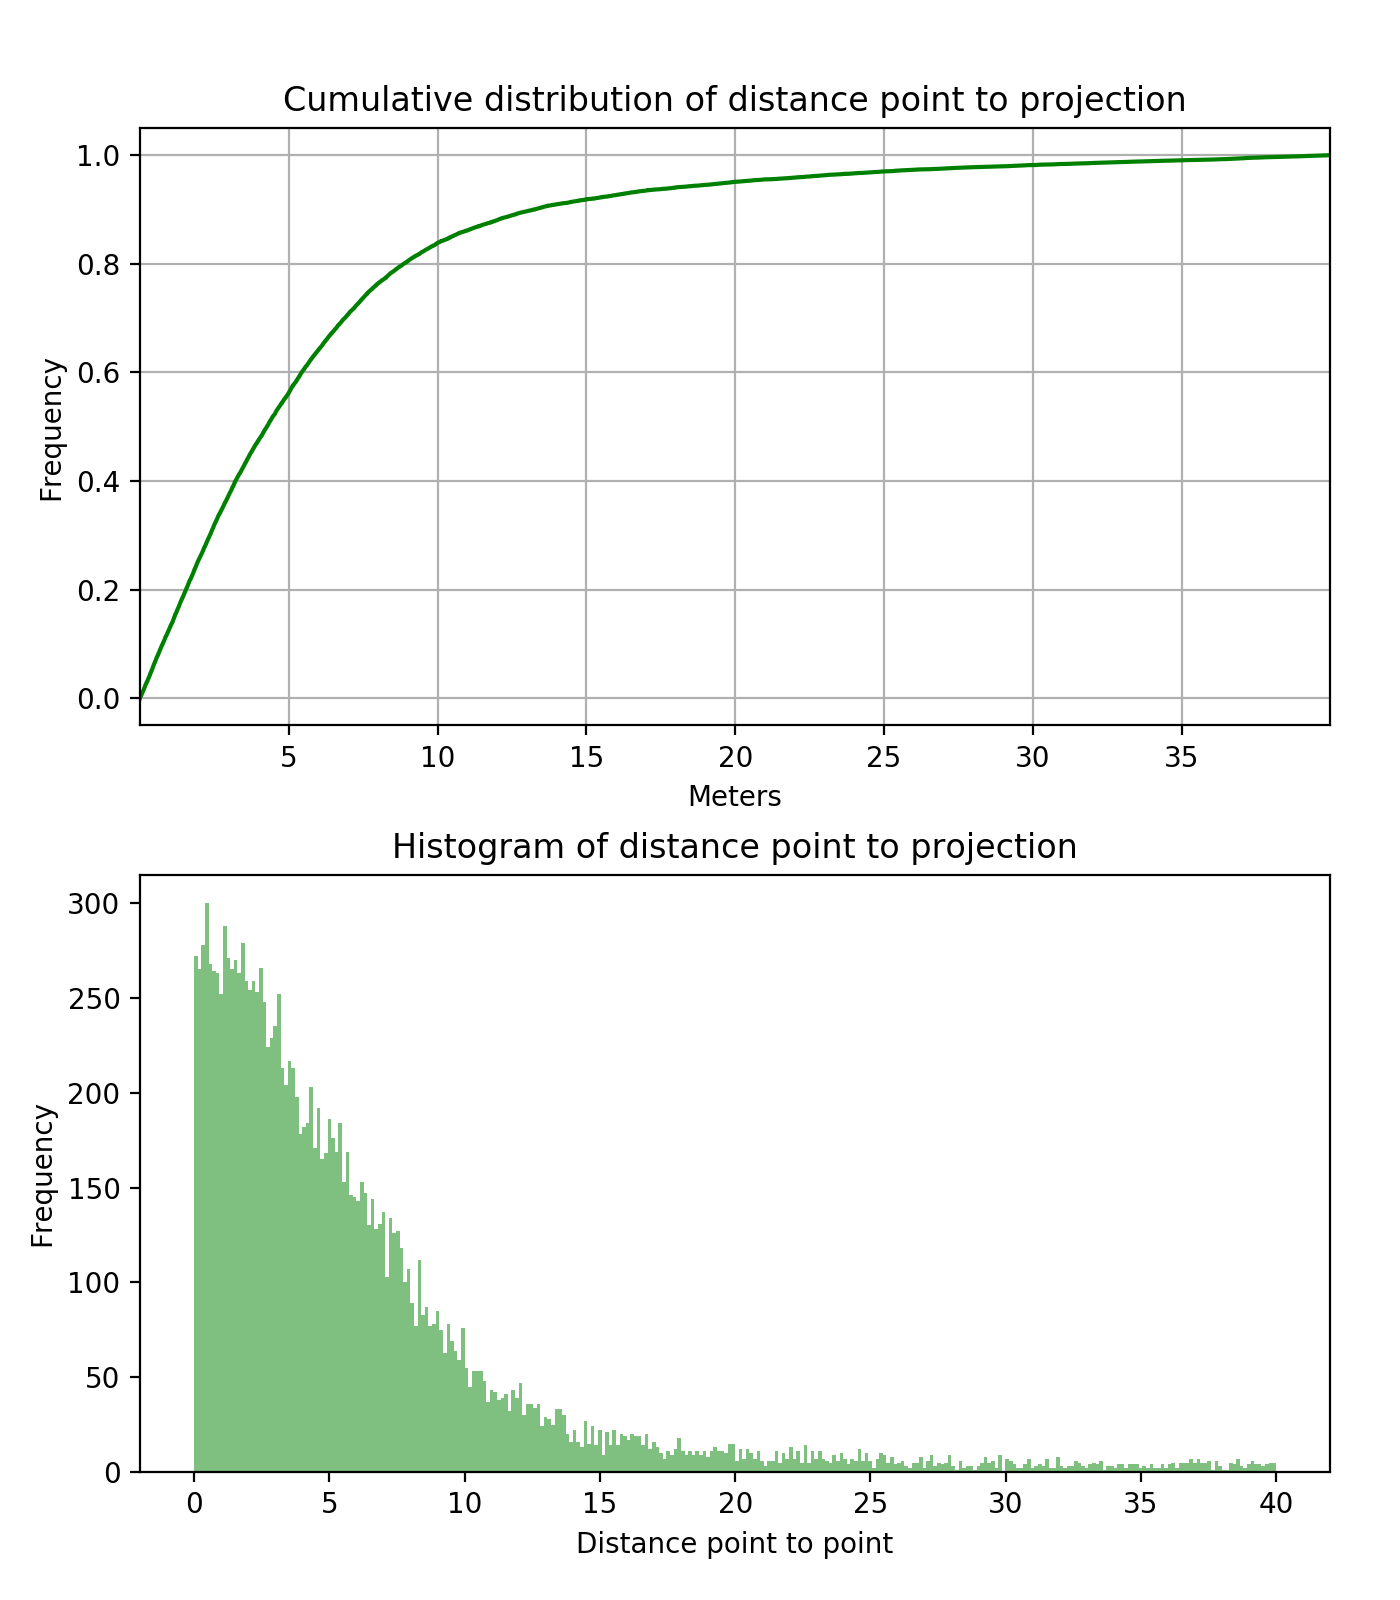
\includegraphics[width=0.9\textwidth]{./Imagenes/PointToProjection.png}
\caption{Muestra de análisis: Distancia punto a proyección.}
\label{figure:PointToProjection}
\end{minipage}\hfill
\begin{minipage}{0.48\textwidth}
\centering
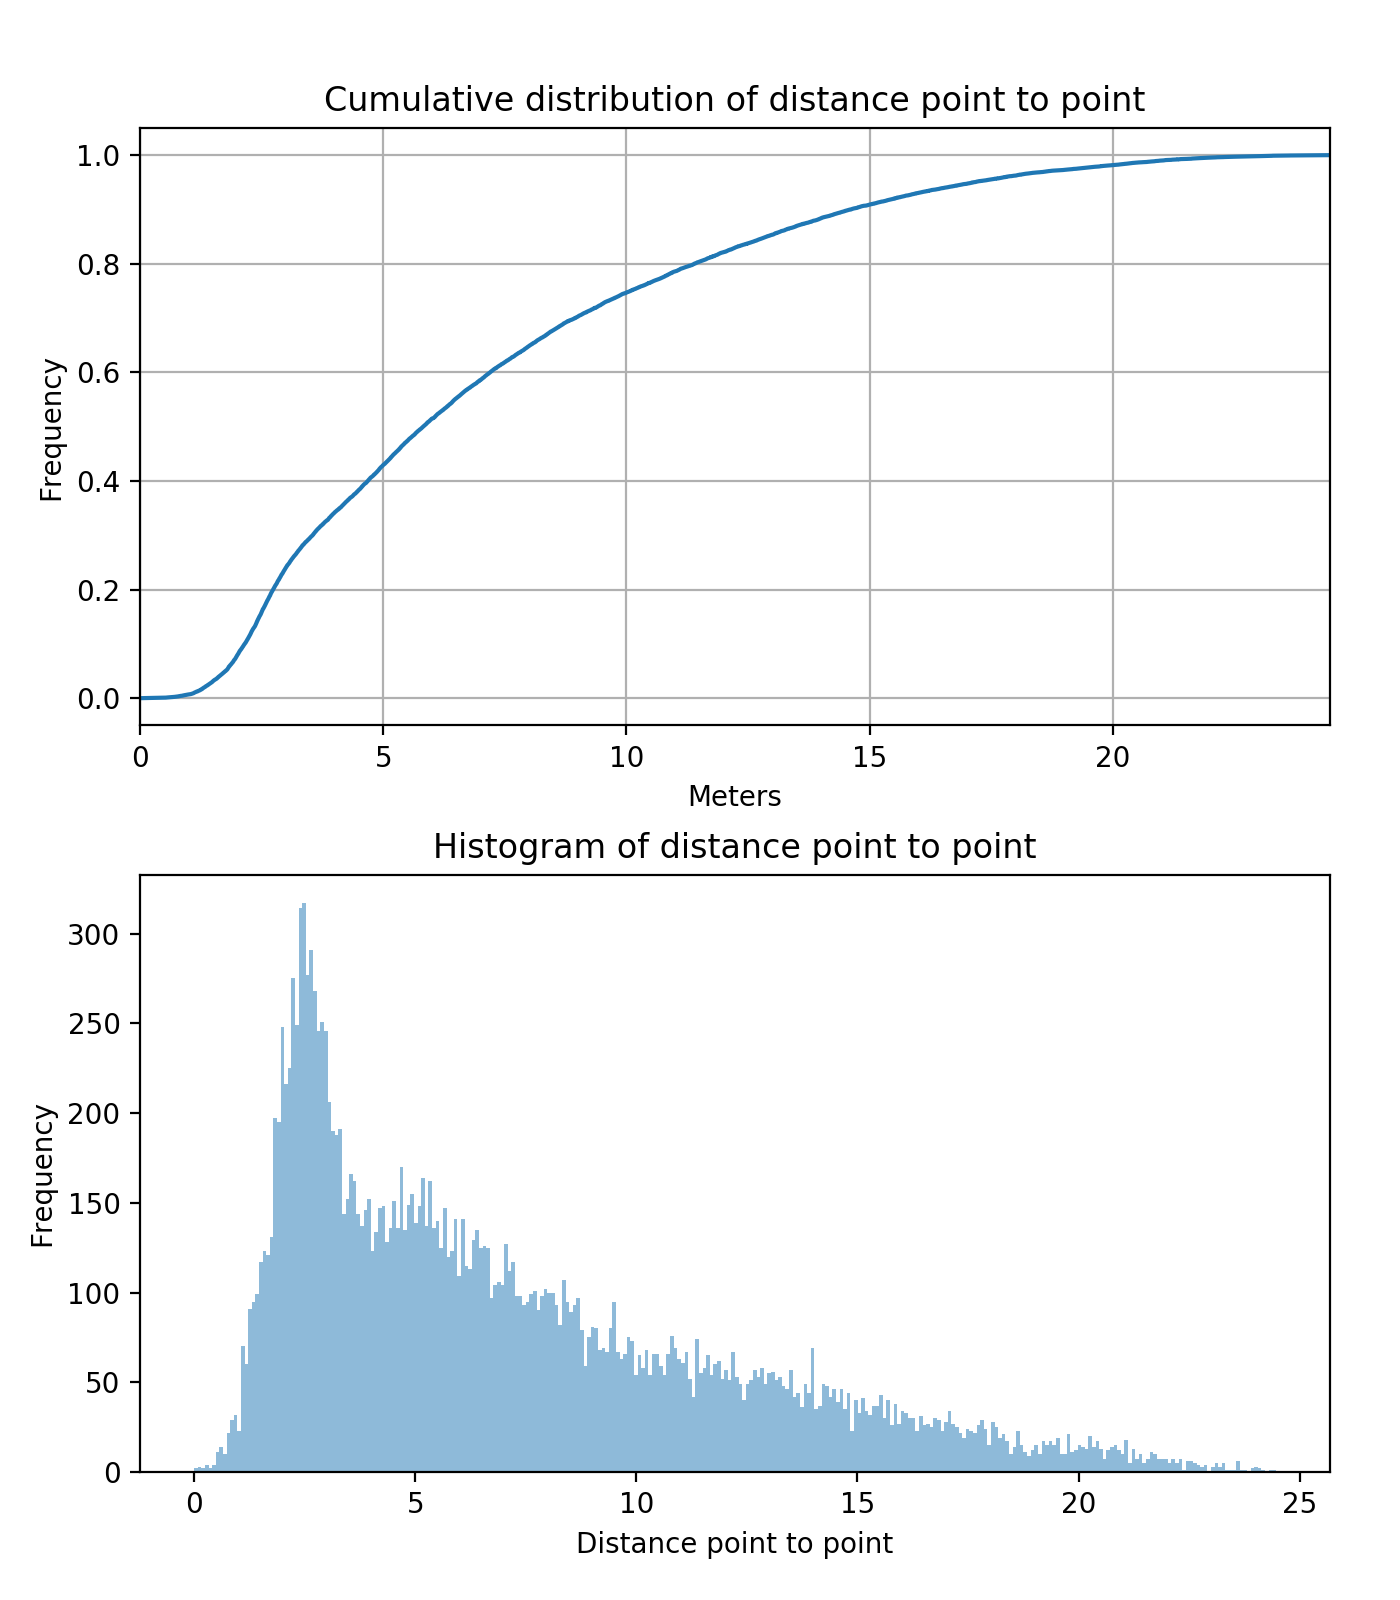
\includegraphics[width=0.9\textwidth]{./Imagenes/PointToPoint.png}
\caption{Muestra de análisis: Distancia punto a punto.}
\label{figure:PointToPoint}
\end{minipage}
\end{figure}
Como se ve en la imagen \ref{figure:PointToProjection} el 80\% de la distancia entre el punto y la 
proyección con el camino correcto está establecido entre 0 y 10 metros dentros.

En la figura \ref{figure:PointToPoint} vemos la información correspondiente a la distancia 
entre un punto $x_{n}$ y el punto $x_{n+1}$. El espectro de distancia en este caso es mayor, 
esto puede debido a la frecuencia del dispositivo, como a la velocidad de individuo, que puede 
variar en función de la pendiente del camino.
%!TeX root=MemoriaTFG.tex

\chapter{Simulación de trayectorias}
Definiremos como simulación de una trayectoria al proceso por el cual, mediante los valores 
medibles y cuantificables extraídos del proceso de análisis, se recrea una trayectoria que cumpla 
los mismos criterios. El proceso de simulación (figura )de esta propuesta tiene dos procesos principales.
Primero se generará el camino dada las probabilidades analizadas desde el nodo inicio seleccionado.
Posteriormente se realizará la simulación de la trayectoria por el camino seleccionado.
\begin{figure}[!htb]
\begin{minipage}{0.48\textwidth}
\centering
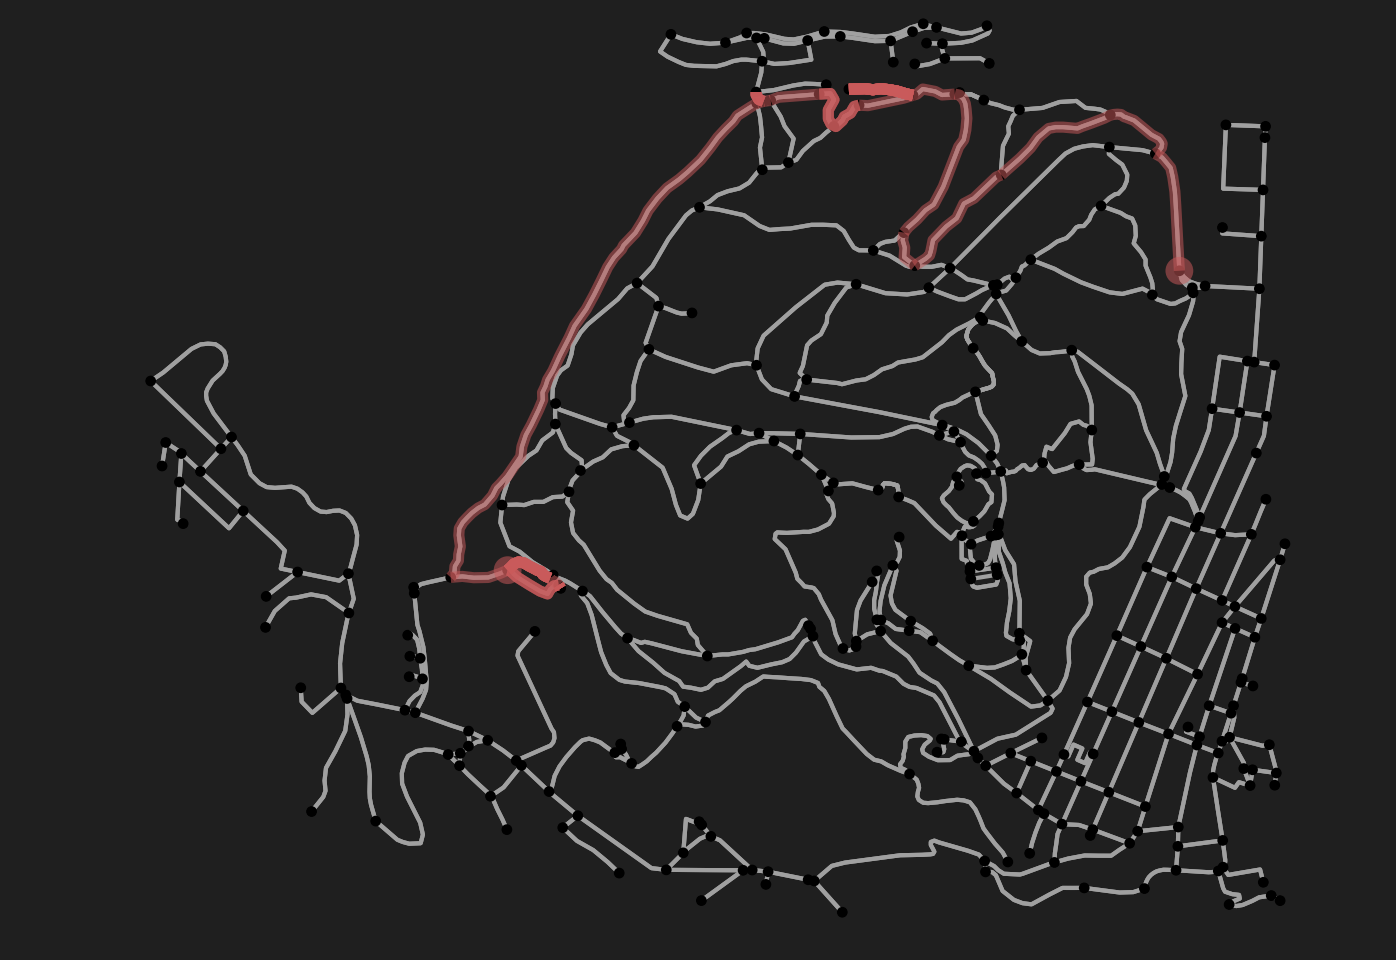
\includegraphics[width=0.9\textwidth]{./Imagenes/TrackGenerationSegments.png}
\caption{Generación de camino.}
\label{figure:PointToProjection}
\end{minipage}\hfill
\begin{minipage}{0.48\textwidth}
\centering
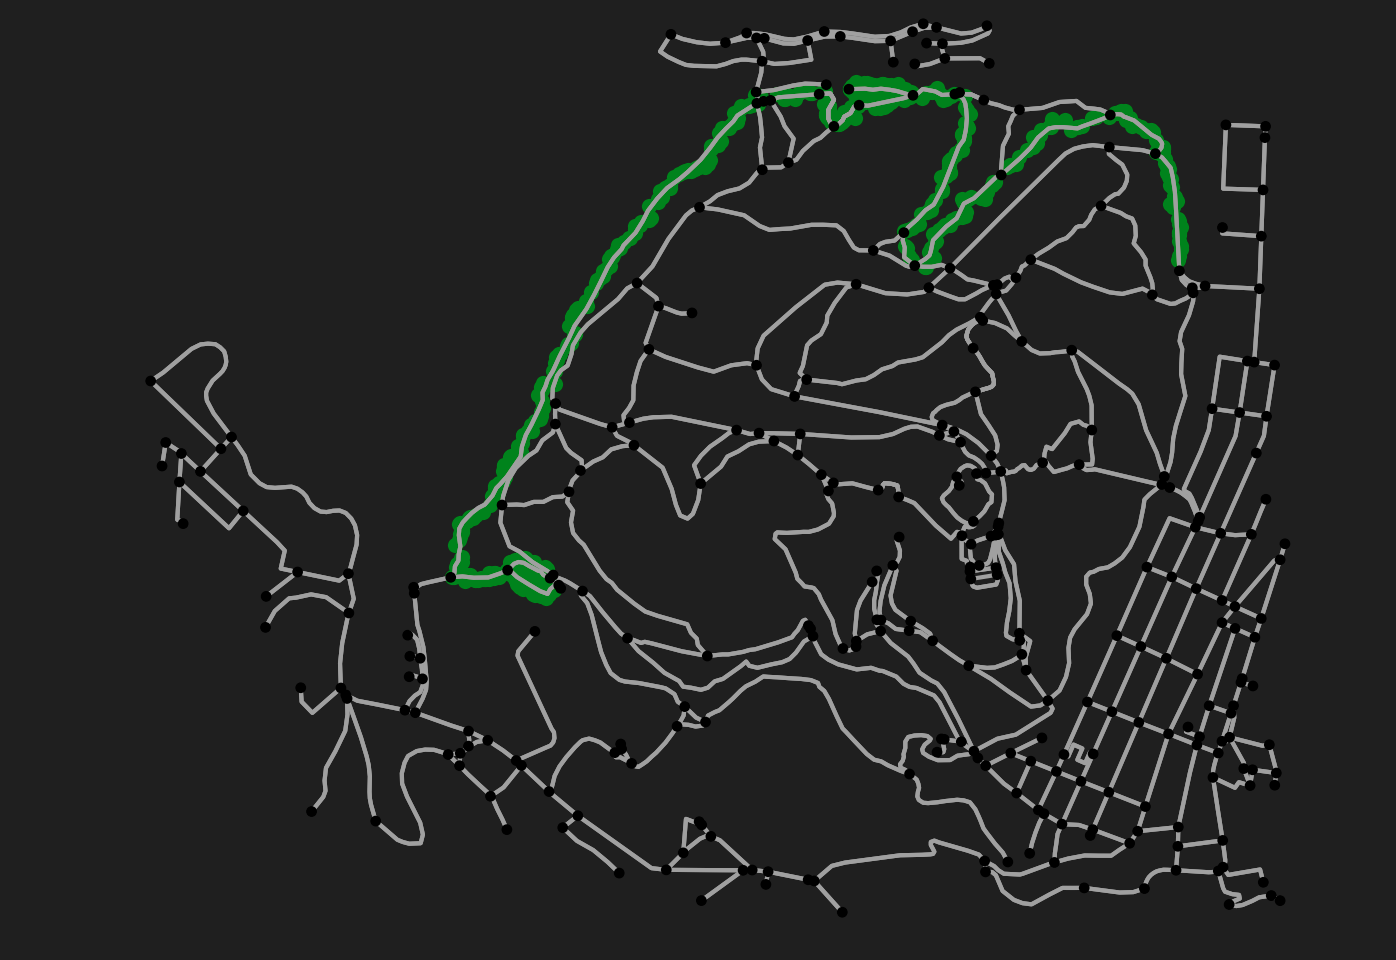
\includegraphics[width=0.9\textwidth]{./Imagenes/TrackGenerationPoints.png}
\caption{Generación de puntos.}
\label{figure:PointToPoint}
\end{minipage}
\end{figure}

\section{Generación de un camino}

La estructura lógica comentada en la sección \ref{section: EstructuraLogica} nos permite 
almacenar en las aristas la información referente a la frecuencia relativa de paso.
Para generar un camino, se realizará un proceso iterativo por el cual mediante un nodo origen, 
asignado por parámetro de entrada, se seleccionará uno de los caminos, manteniendo la 
distribución probabilística del conjunto de aristas, de forma que si una de las aristas tiene una 
frecuencia del 25\% de las detecciones, con un número suficiente de muestras se cumpliría dicha 
distribución. 
\begin{figure}[!htb]
\begin{center}
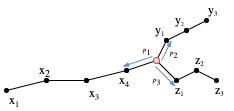
\includegraphics[width=0.75\textwidth]{./Imagenes/SimulationProbabilities.png}
\caption{Ejemplo de probabilidades dentro de un nodo intermedio entre rutas.}
\label{fig:PointGeneration02}
\end{center}
\end{figure}

El proceso de selección de aristas continuará hasta que la suma de las distancias 
acumule el total de distancia por recorrer, que será otro de los parámetros de entrada.
La implementación de este proceso se encuentra en el método \textit{create\_path} de la 
implementación del \textbf{\textit{interactor}} \textit{simulate\_track\_impl}

\begin{lstlisting}[caption={Método create\_path}\label{algoritmo:create_path},language=Python] 
    def create_path(self, origin, dist):
        path = []
        distance_created = 0
        prev_node = origin
        path.append(origin)
        while distance_created < dist:
            next_node = self.get_most_frequent_node(prev_node, path)
            distance_aux = distance_created + self.graph.get_edge_by_nodes(prev_node, next_node)['length']
            if distance_aux < dist:
                distance_created = distance_aux
                path.append(next_node)
                prev_node = next_node
            else:
                return path, distance_created
        return path, distance_created
\end{lstlisting}

\section{Generación de los segmentos}

Una vez se tiene seleccionado el camino que se realizará. Se simulará cada uno de los segmentos individualmente.
Para ello se identificara el nodo origen y final del segmento y se generarán todos los puntos necesarios hasta
que la distancia a ese punto sea menor a una $d$, donde $d$ es una distancia parametrizada y modificable. 
La implementación de este proceso se encuentra en el método \textit{simulate\_segment} de la implementación 
del \textbf{\textit{interactor}} \textit{simulate\_track\_impl}

\begin{lstlisting}[caption={Método simulate\_segment}\label{algoritmo:simulateSegment},language=Python] 
    def simulate_segment(self, segment):
        aux = 0
        origin_node = segment[0]
        target_node = segment[1]
        segment = []
        origin_point = TrackPoint(self.graph.get_nodes()[origin_node]['x'], self.graph.get_nodes()[origin_node]['y'])
        target_point = TrackPoint(self.graph.get_nodes()[target_node]['x'], self.graph.get_nodes()[target_node]['y'])
        try:
            dest, aux = self.calculate_point(segment, origin_node, target_node, origin_point, target_point)
            next = dest
            while aux > DISTANCE_TO_FINAL_NODE:
                dest, aux = self.calculate_point(segment, origin_node, target_node, next, target_point)
                next = dest
        except KeyError:
            pass
        return segment
\end{lstlisting}

\newpage
\section{Generación del punto pseudo-aleatorio}

Es en este punto de la lógica donde se realiza la generación de puntos de forma pseudo-aleatoria, 
utilizando información procedente de los análisis realizados.
Para la creación de un punto a partir de otro se necesita una distancia $d$ y un ángulo $\alpha$ como 
se muestra en la figura \ref{fig:PointGeneration01}
\begin{figure}[htb]
\begin{center}
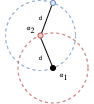
\includegraphics[scale=0.75, width=0.3\textwidth]{./Imagenes/PointGeneration01.png}
\caption{Ejemplo de generación de punto a partir de una distancia $d$ y un ángulo $\alpha$.}
\label{fig:PointGeneration01}
\end{center}
\end{figure}

Cada punto sera generado teniendo en cuenta el punto anterior. Se encontrará la proyección del segmento
más cercano y se centrará el ángulo en el nodo inmediatamente posterior, con una desviación $\beta$ 
parametrizada y modificable. El proceso queda ilustrado en la figura \ref{fig:PointGeneration02}

\begin{figure}[htb]
\begin{center}
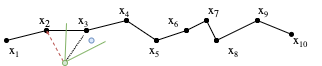
\includegraphics[width=0.75\textwidth]{./Imagenes/PointGeneration02.png}
\caption{Ejemplo de detección de proyección cercana y generación de punto.}
\label{fig:PointGeneration02}
\end{center}
\end{figure}

La distancia para la generación del punto se obtendrá de una elección aleatoria siguiendo un proceso 
llamado \textit{Inverse transform sampling}, por el que se genera un número pseudo-aleatorio a partir 
de una función acumulativa dada una distribución probabilística \cite{Sigman01}.

La distribución probabilística de la distancia punto a punto se obtiene a partir de la información 
que se genera en el proceso de análisis. Se puede ver un ejemplo en la figur 
\ref{figure:PointToPoint} mostrada en la sección \ref{section: AnalisisDistancias}.

\section{Exportación de trayectoria a fichero .\ac{GPX}}
En esta sección se pretende describir la característica del aplicativo para realizar la exportación a GPX.

%!TeX root=MemoriaTFG.tex
\chapter{Experimentacion}
En este capítulo se documentan las pruebas realizadas al aplicativo propuesto con el objetivo de analizar los resultados obtenidos del análisis y la simulación.
Esta experimentación parte de unas condiciones generales. Contamos con un total de 25 rutas reales realizadas en el territorio delimitado del Castell de Bellver (Mallorca). Para la realización de la experimentación contamos con un número reducido de muestras. Para que el resultado del análisis pueda representar un comportamiento destacable se han replicado las mismas rutas un total de 7 veces, contando entonces con un total de más de 200 trayectorias, de una muestra inicial de 30. De esta forma alimentamos el modelo con una cantidad de información suficiente para apreciar resultados. Estas condiciones de entrada parten de la necesidad de alimentar el modelo con una información que pueda llegar a ser representativa.

En la figura \ref{figure:RealHeatMap} se muestra el mapa de calor resultado del proceso de análisis:
\begin{figure}[!htb]
\begin{center}
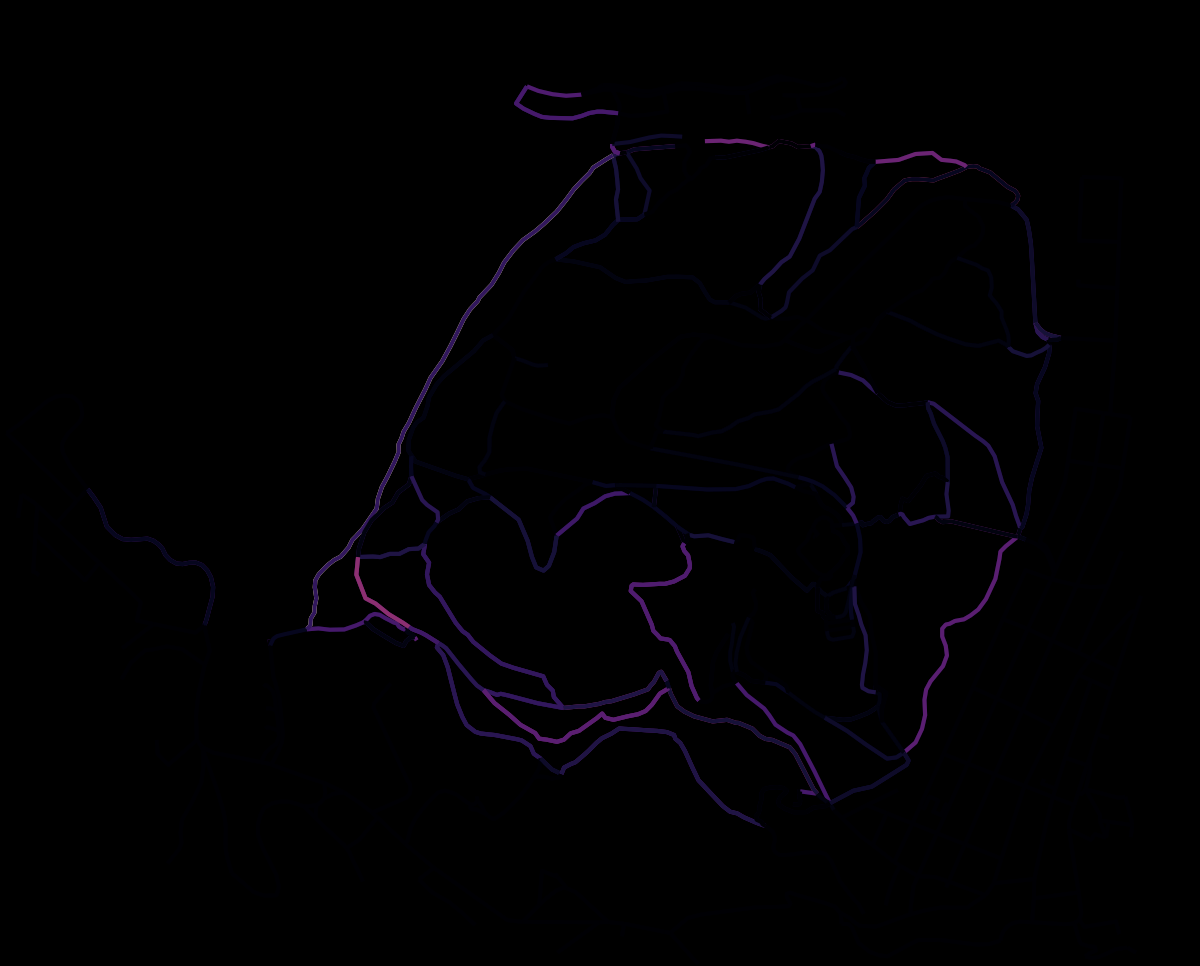
\includegraphics[width=0.7\textwidth]{./Imagenes/HeatMap.png}
\caption{Mapa de calor del conjunto de rutas reales.}
\label{figure:RealHeatMap}
\end{center}
\end{figure}
\newpage
Este mapa representa la frecuencia de paso del individuo por cada uno de los caminos establecidos en 
el territorio. Colores oscuros representarían frecuencias bajas y el color cobra una tonalidad rojiza a 
medida que la frecuencia sería mayor.

Se observa que el individuo ha realizado uso mayor del perímetro del bosque del territorio. Esto 
concuerda con la visualización de las rutas individuales. Con un conjunto mayor de datos, el mapa de 
calor llegaría a mostrar colores rojizos.

Las pruebas que realizaremos se basan en dos vertientes. Por una parte se realiza un análisis de una 
generación de rutas donde no se han importado datos reales. Por otro parte se realiza un análisis de 
rutas simuladas con datos reales introducidos en el modelo.


\section{Experimentación sin importación de datos reales}
En este apartado realiza la muestra de resultados de la generación de 10 rutas creadas 
mediante la simulación sin datos de análisis almacenados. Al no tener datos almacenados dentro del 
sistema la simulación corresponderá a una elección aleatoria del los diferentes caminos ya que, por 
defecto, todos los caminos tienen la misma probabilidad de tránsito a falta de introducir datos en el 
modelo. Por otra parte la distancia punto a punto será una constante definida en 20 metros, por lo 
que no aparecerá variabilidad en la muestra. Esta constante está parametrizada y puede ser 
modificable por el usuario.
Se han realizado una simulación de 10 rutas. Una muestra de estas simulaciones las podemos encontrar en el apartado \ref{subseciton:SimulationSample}. Las figuras \ref{figure:SimulatedTrack1}, \ref{figure:SimulatedTrack2} y \ref{figure:SimulatedTrack3} son son ejemplos de estas simulaciones.
\begin{figure}[!htb]
\centering
\begin{minipage}{0.70\textwidth}
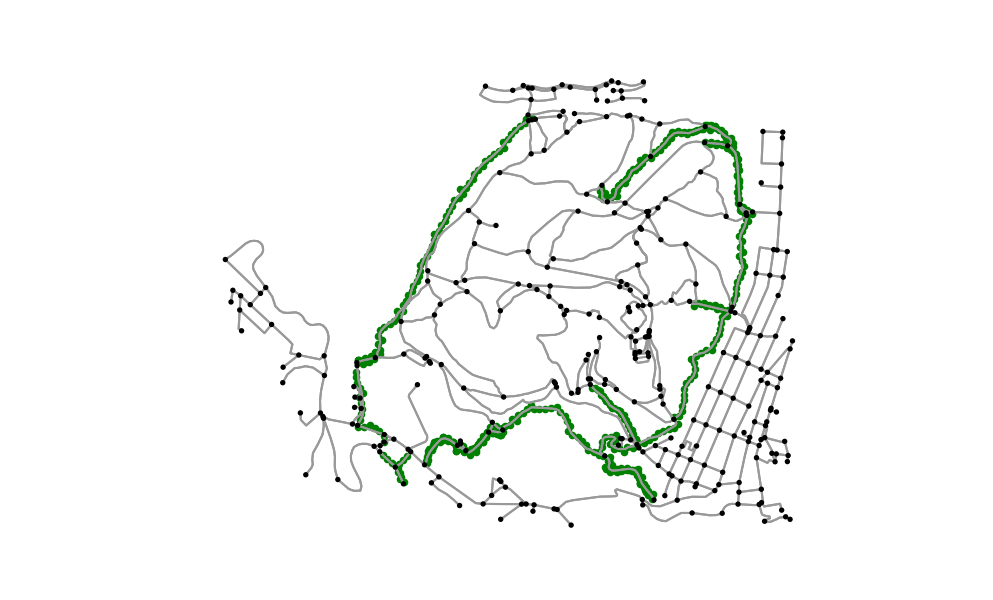
\includegraphics[width=0.9\textwidth]{./Imagenes/SimulatedTrack1Empty.png}
\caption{Muestra de simulación 1 (Experimentación sin datos).}
\label{figure:SimulatedTrack1}
\end{minipage}
\begin{minipage}{0.48\textwidth}
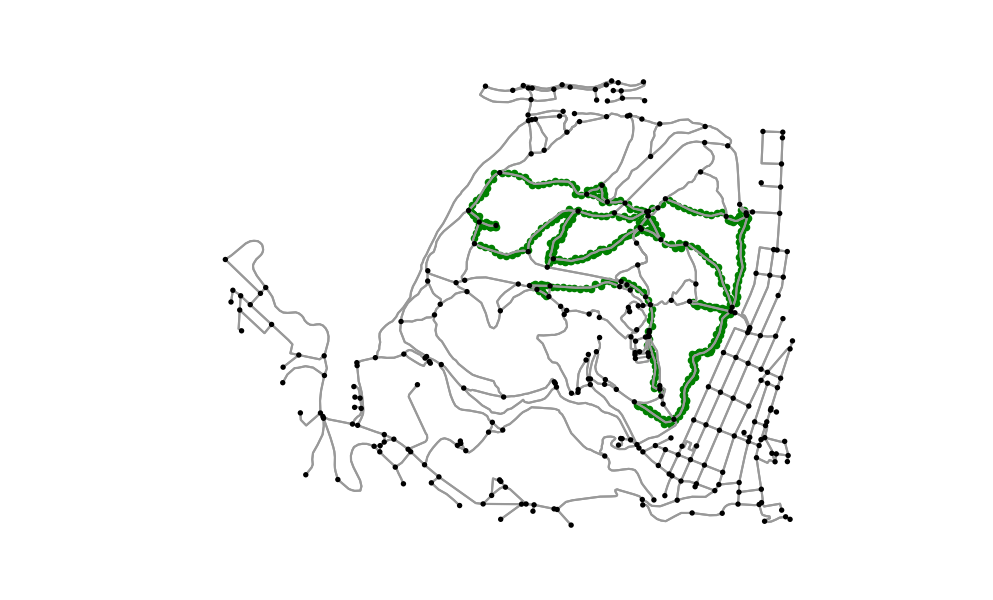
\includegraphics[width=0.9\textwidth]{./Imagenes/SimulatedTrack2Empty.png}
\caption{Muestra de simulación 2 (Experimentación sin datos).}
\label{figure:SimulatedTrack2}
\end{minipage}
\hfill 
\begin{minipage}{0.48\textwidth}
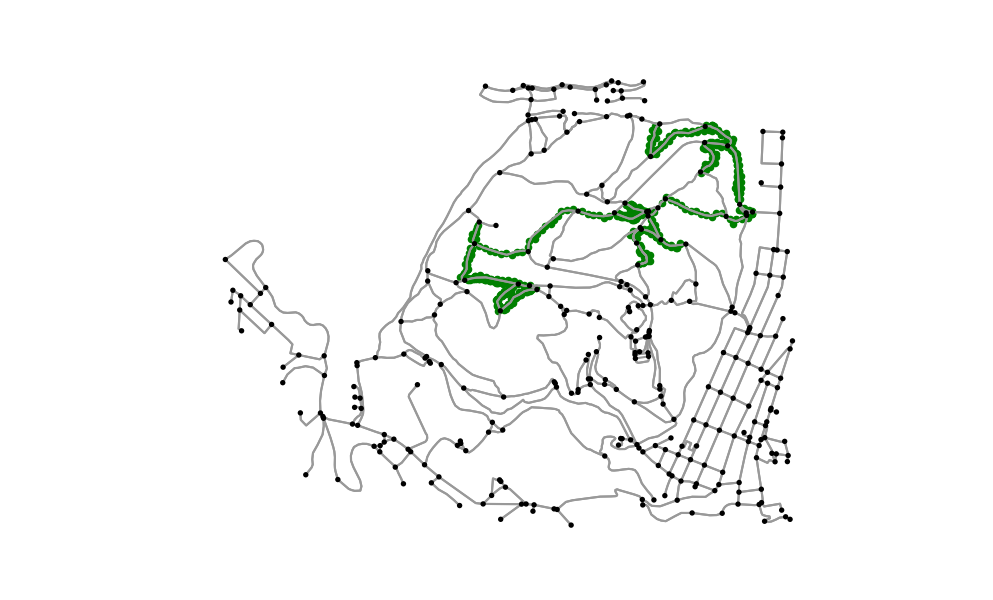
\includegraphics[width=0.9\textwidth]{./Imagenes/SimulatedTrack3Empty.png}
\caption{Muestra de simulación 3 (Experimentación sin datos).}
\label{figure:SimulatedTrack3}
\end{minipage}
\end{figure}
\newpage

Por una parte, en el mapa de calor resultante (figura \ref{figure:SimulatedHeatMapEmpty}) no se 
observan patrones observables, esto es debido a la elección pseudo-aleatoria de cada uno de los 
segmentos seleccionados.

\begin{figure}[!htb]
\begin{center}
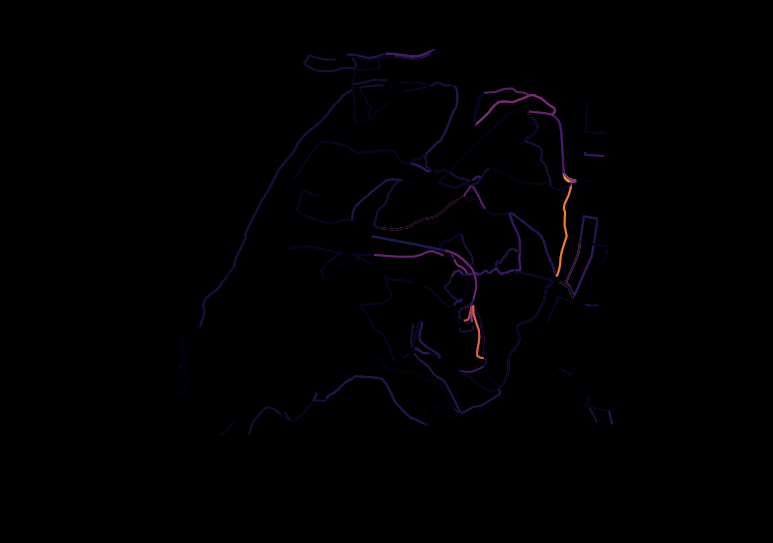
\includegraphics[width=0.7\textwidth]{./Imagenes/HeatMapEmpty.png}
\caption{Mapa de calor del conjunto de rutas simuladas en experimentación sin datos.}
\label{figure:SimulatedHeatMapEmpty}
\end{center}
\end{figure}
\newpage
Las distribuciones se observan constantes al valor parametrizado al que están asignados en caso 
de que no se encuentren datos para realizar la simulación (figura \ref{figure:SimulatedPointToPointEmpty}) por 
otra parte se observa la aletoriedad en forma de distribución normal de la distancia punto a proyección, que no 
corresponde a ningún comportamiento parametrizado (figura \ref{figure:SimulatedPointToProjectionEmpty}).
\begin{figure}[!htb]
\begin{minipage}{0.48\textwidth}
\centering
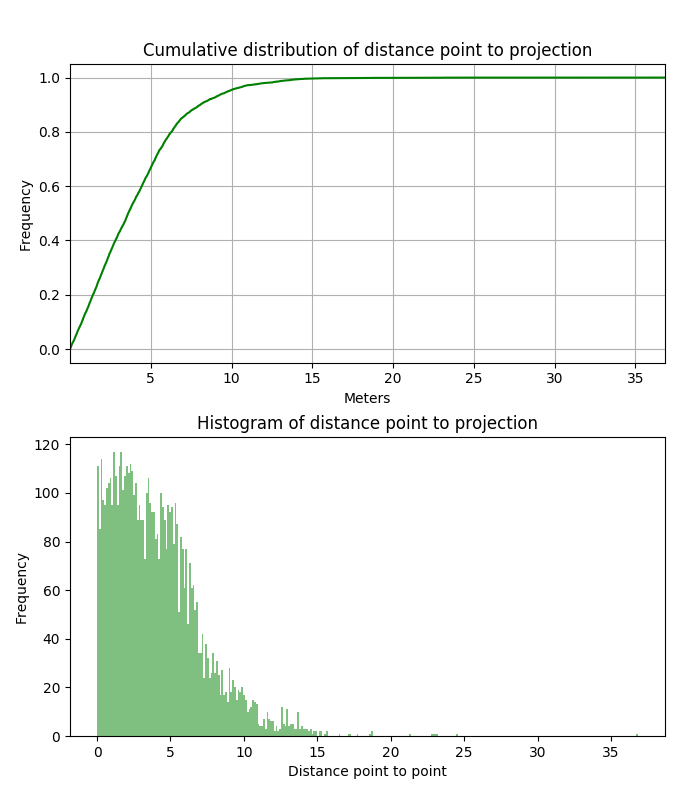
\includegraphics[width=1.2\textwidth]{./Imagenes/SimulateCumulativePointProjectionEmpty.png}
\caption{Muestra de análisis de simulación: Distancia punto a proyección en experimentación sin datos.}
\label{figure:SimulatedPointToProjectionEmpty}
\end{minipage}\hfill
\begin{minipage}{0.48\textwidth}
\centering
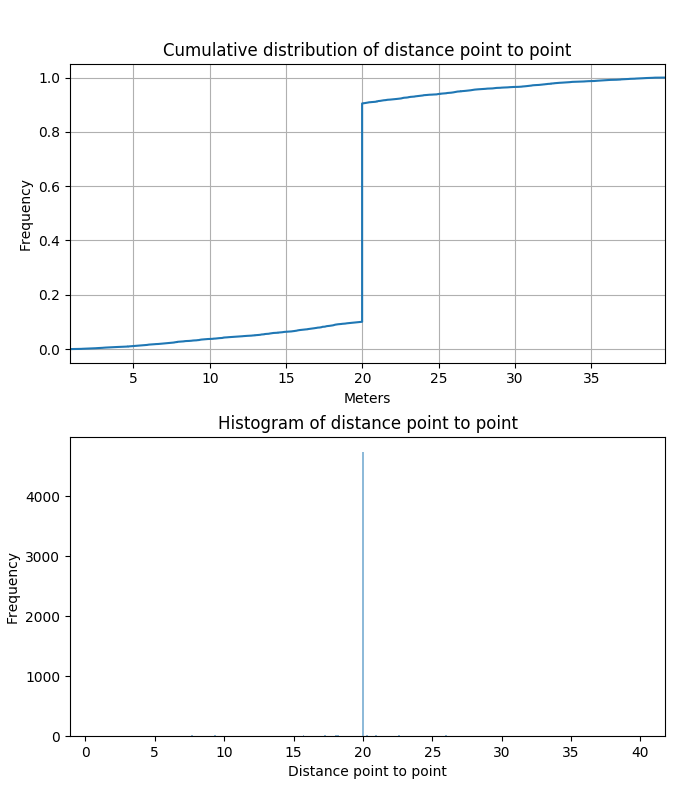
\includegraphics[width=1.2\textwidth]{./Imagenes/SimulateCumulativePointPointEmpty.png}
\caption{Muestra de análisis de simulación: Distancia punto a punto en experimentación sin datos.}
\label{figure:SimulatedPointToPointEmpty}
\end{minipage}
\end{figure}


\section{Experimentación con importación de datos reales}
Para la simulación, se ha alimentado al modelo con el análisis de las rutas reales de 10 km de distancia sobre 
el territorio del Castell de Bellver. Todas parten del origen de la entrada nordeste del recinto. Se han generado un total de 253 rutas. Posteriormente estas rutas han sido pasadas por el analizador con el objetivo de valorar si mantienen la misma distribución en las variables respecto el análisis de las rutas reales. Las figuras \ref{figure:SimulatedTrack1}.
\begin{figure}[!htb]
\centering
\begin{minipage}{0.70\textwidth}
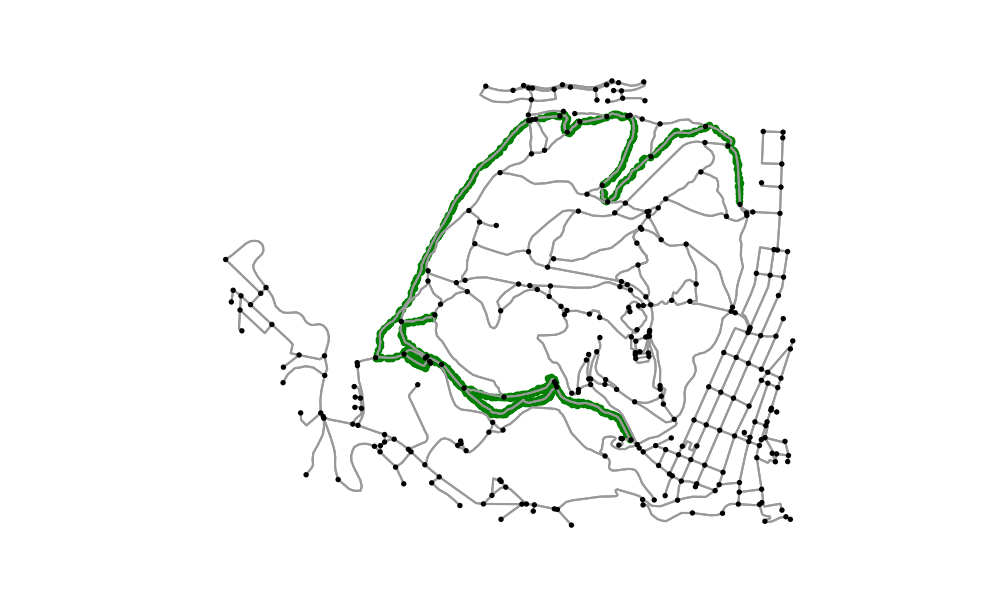
\includegraphics[width=0.9\textwidth]{./Imagenes/SimulatedTrack1.png}
\caption{Muestra de simulación 1 Experimentación con datos).}
\label{figure:SimulatedTrack1}
\end{minipage}
\begin{minipage}{0.48\textwidth}
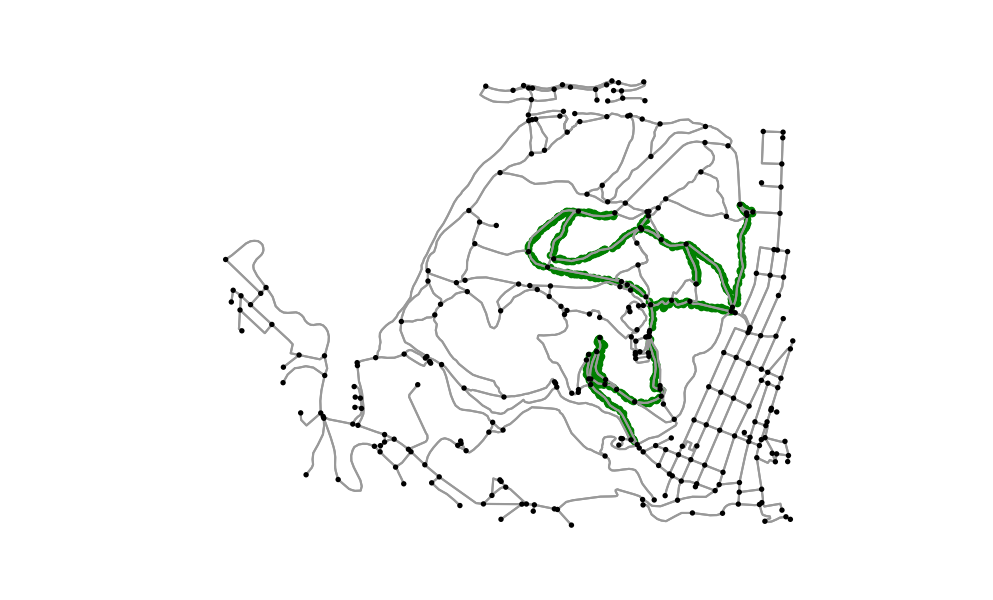
\includegraphics[width=0.9\textwidth]{./Imagenes/SimulatedTrack2.png}
\caption{Muestra de simulación 2 Experimentación con datos).}
\label{figure:SimulatedTrack2}
\end{minipage}
\hfill 
\begin{minipage}{0.48\textwidth}
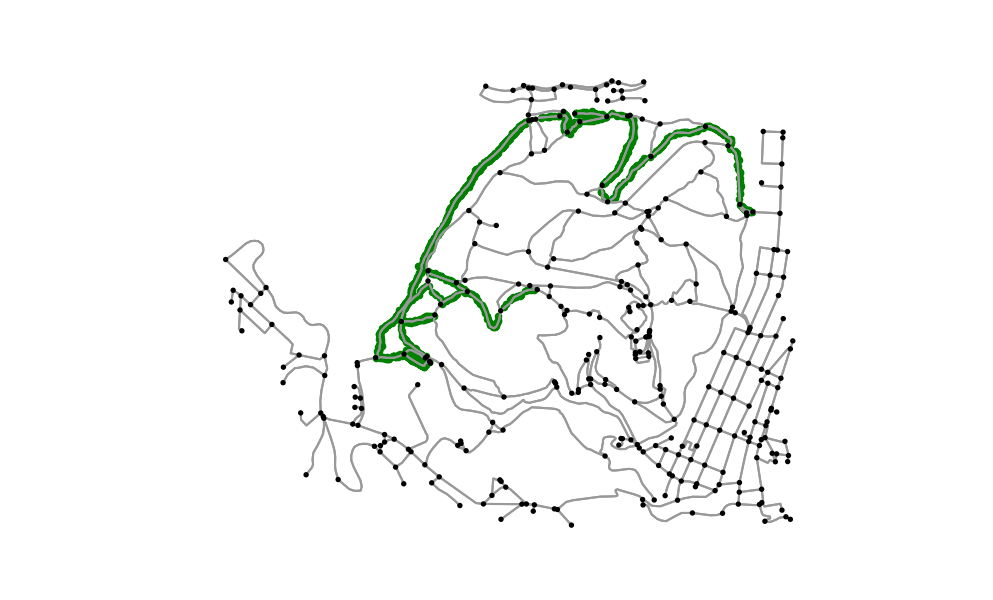
\includegraphics[width=0.9\textwidth]{./Imagenes/SimulatedTrack3.png}
\caption{Muestra de simulación 3 (Experimentación con datos).}
\label{figure:SimulatedTrack3}
\end{minipage}
\end{figure}
\newpage

La figura \ref{figure:SimulatedHeatMap} corresponde al mapa de calor del análisis de las generaciones. Se puede observar una trayectoria más definida, que se corresponde con el mapa de calor mostrado 
anteriormente en la figura \ref{figure:RealHeatMap}.
\begin{figure}[!htb]
\begin{center}
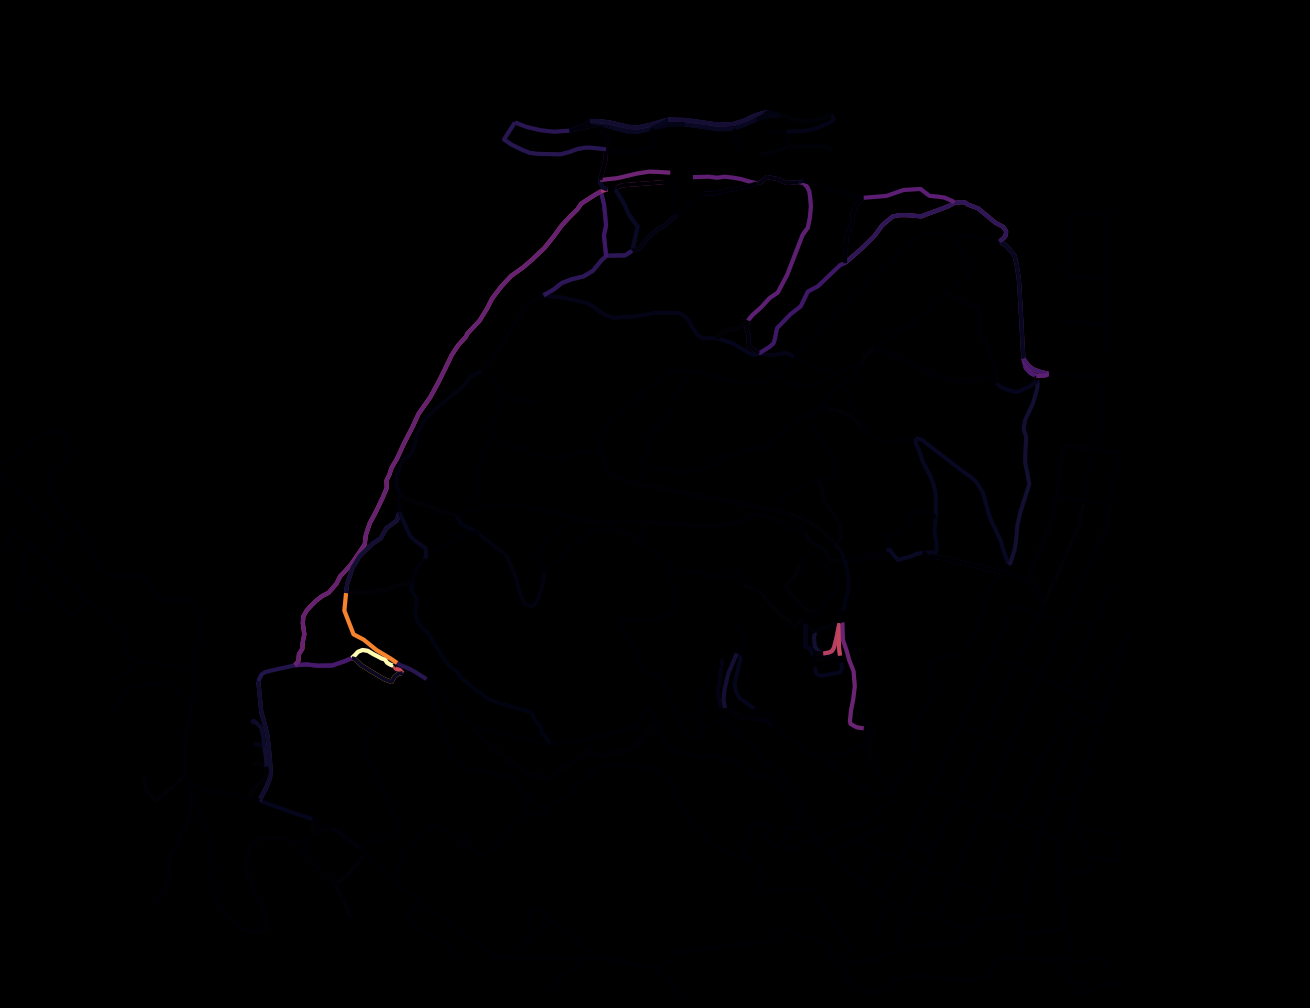
\includegraphics[width=0.7\textwidth]{./Imagenes/SimulatedHeatMap1.png}
\caption{Mapa de calor del conjunto de rutas simuladas en experimentación con datos.}
\label{figure:SimulatedHeatMap}
\end{center}
\end{figure}
Existen diversos aspectos que explican las diferencias entre los mapas de calor de las figuras \ref{figure:RealHeatMap} y \ref{figure:SimulatedHeatMap}. Las rutas simuladas tienen una distancia de 
10 kilometros, por lo que hacen inaccessibles ciertos caminos. Se aprecia que la parte norte y este del 
perímetro del bosque del Castell de Bellver es la zona más frecuente, que corresponde con las muestras 
reales. No obstante existen rutas que acceden a la parte sur del camino, con menos frecuencia, por lo 
que no son distingibles.
Las distribuciones corresponden. A nivel de distancia punto a punto se respeta completamente, en la 
distancia punto proyección encontramos una distribución normal mucho más acentuada.

\begin{figure}[!htb]
\begin{minipage}{0.48\textwidth}
\centering
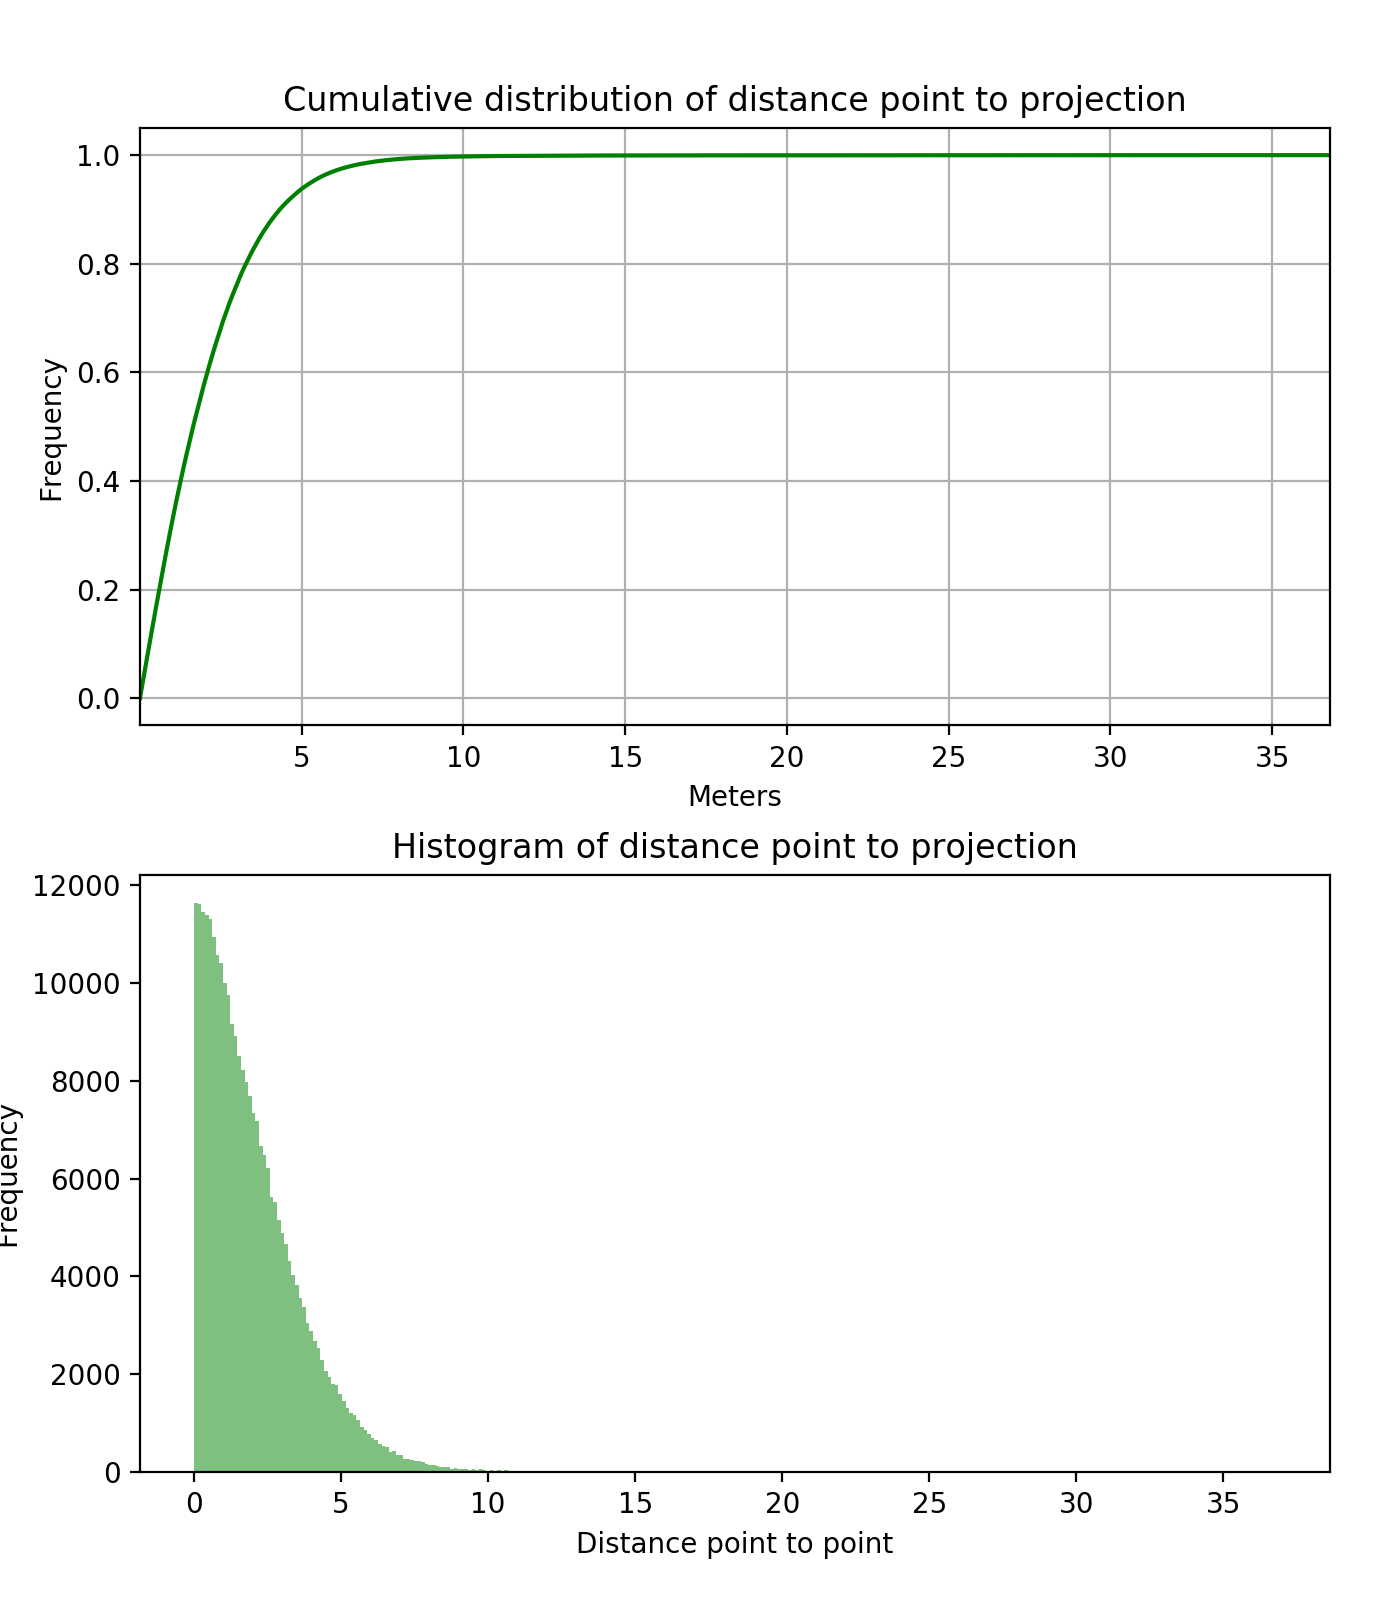
\includegraphics[width=1.2\textwidth]{./Imagenes/SimulateCumulativePointProjection.png}
\caption{Muestra de análisis de simulación: Distancia punto a proyección en experimentación con datos.}
\label{figure:SimulatedPointToProjection}
\end{minipage}\hfill
\begin{minipage}{0.48\textwidth}
\centering
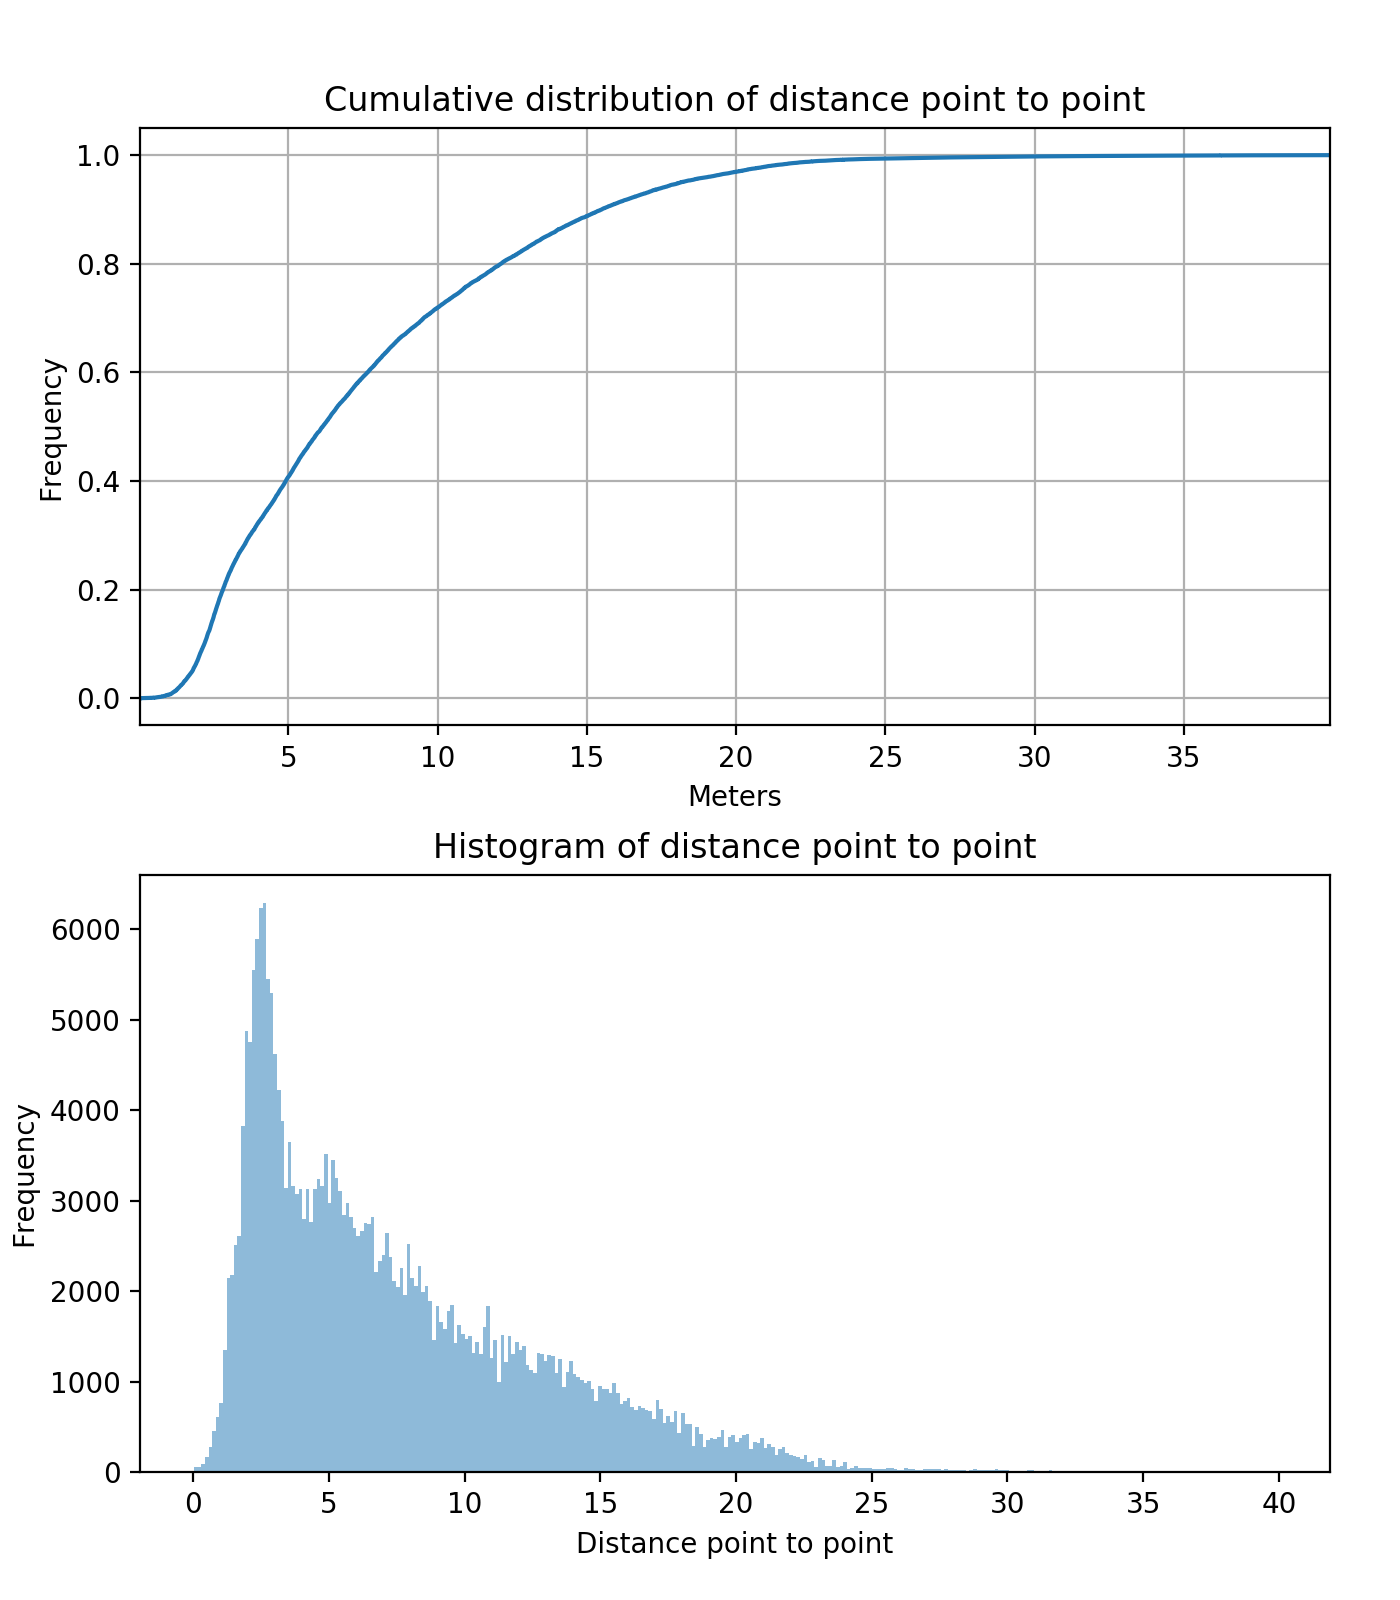
\includegraphics[width=1.2\textwidth]{./Imagenes/SimulateCumulativePointPoint.png}
\caption{Muestra de análisis de simulación: Distancia punto a punto en experimentación con datos.}
\label{figure:SimulatedPointToPoint}
\end{minipage}
\end{figure}
\newpage

\subsection{Comparativa de resultados}
En las figuras \ref{figure:ComparativaReal} y \ref{figure:ComparativaEmpty} se observan los resultados de la distancia punto a punto entre y la comparativa con la distribución real. Se observa que con el uso de los datos 
procedentes del análisis se obtiene una distribución probabilística similar a la distribución real, mientras que 
sin estos datos, aparece una distribución única al valor parametrizado, en este caso 20 metros.

\begin{figure}[!htb]
\begin{minipage}{0.48\textwidth}
\centering
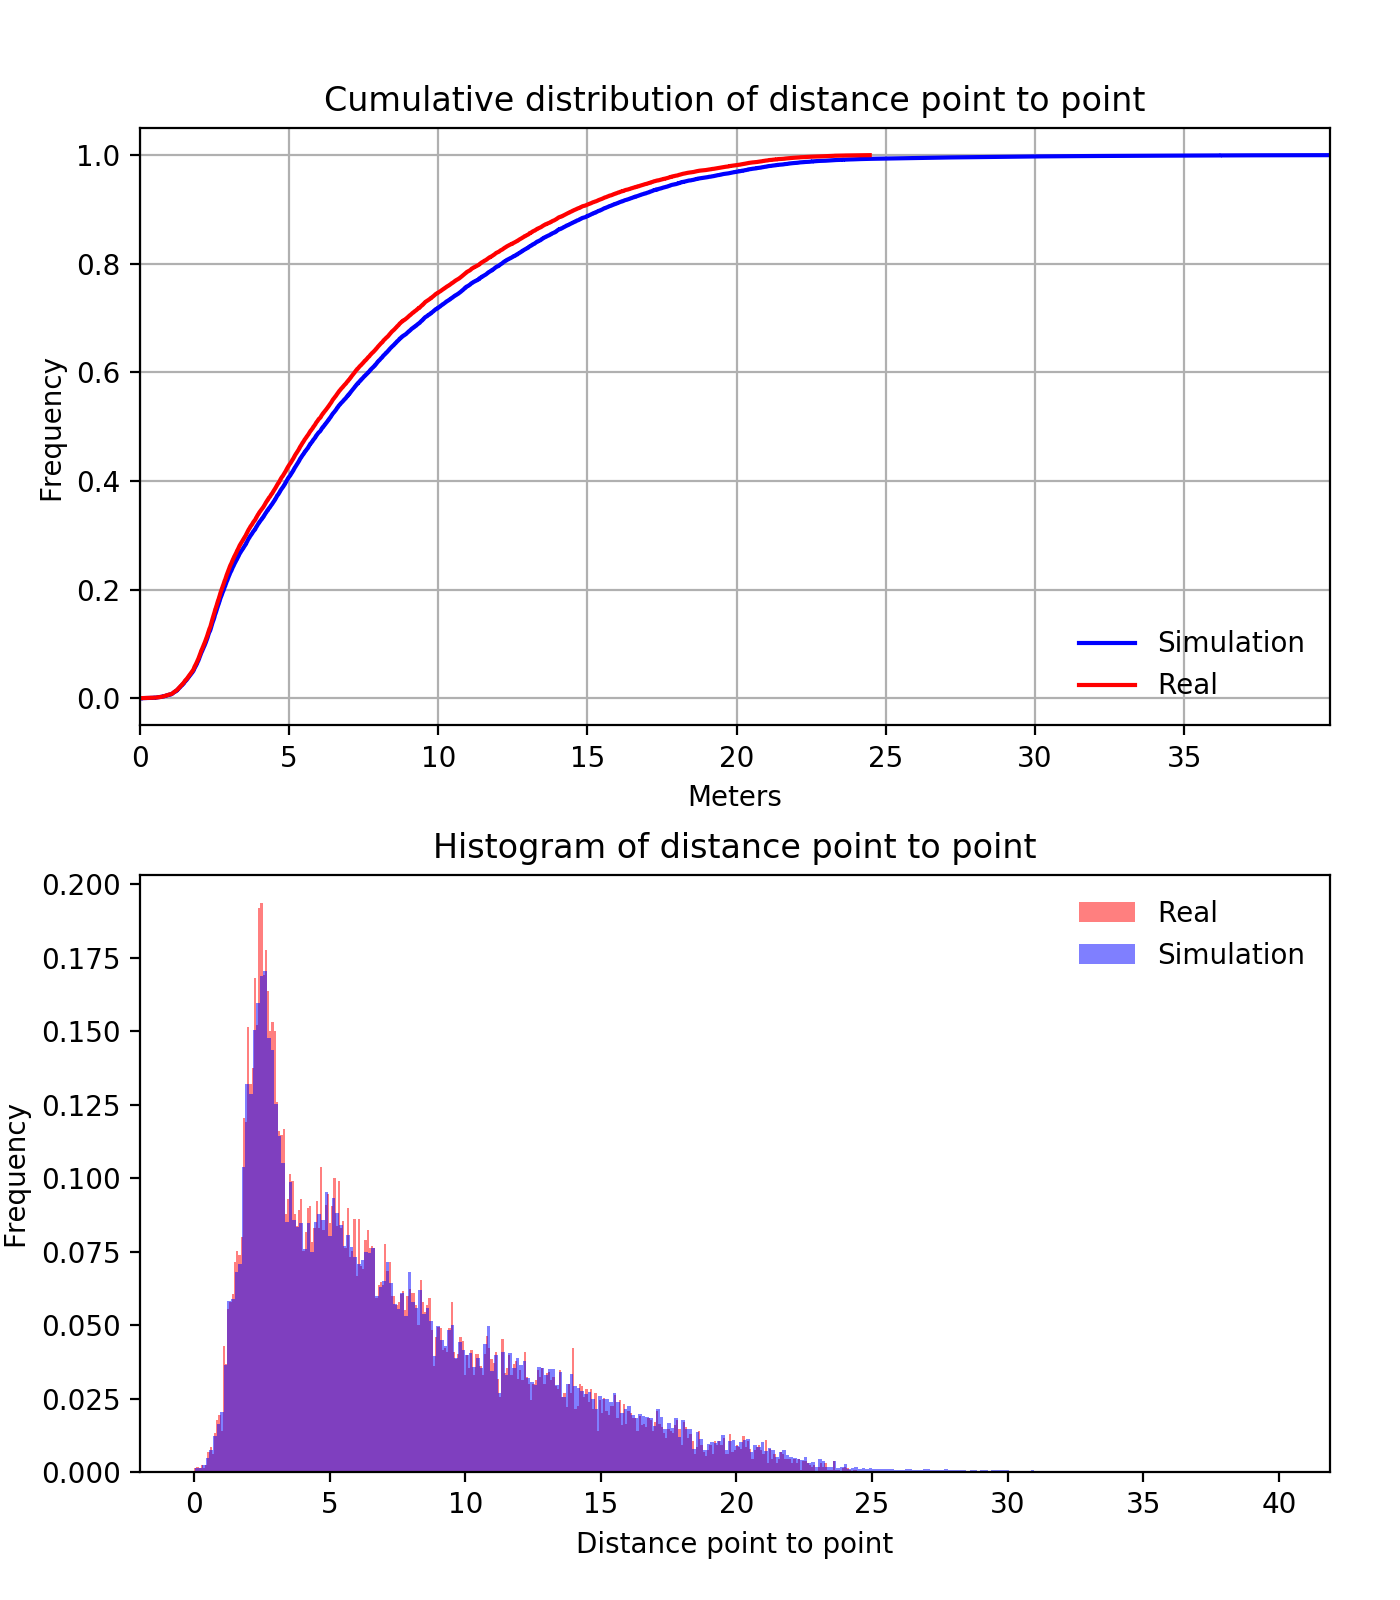
\includegraphics[width=1.2\textwidth]{./Imagenes/SimulationComparativeNormalized.png}
\caption{Comparativa análisis de la distancia punto a proyección en simulación con datos.}
\label{figure:ComparativaReal}
\end{minipage}\hfill
\begin{minipage}{0.48\textwidth}
\centering
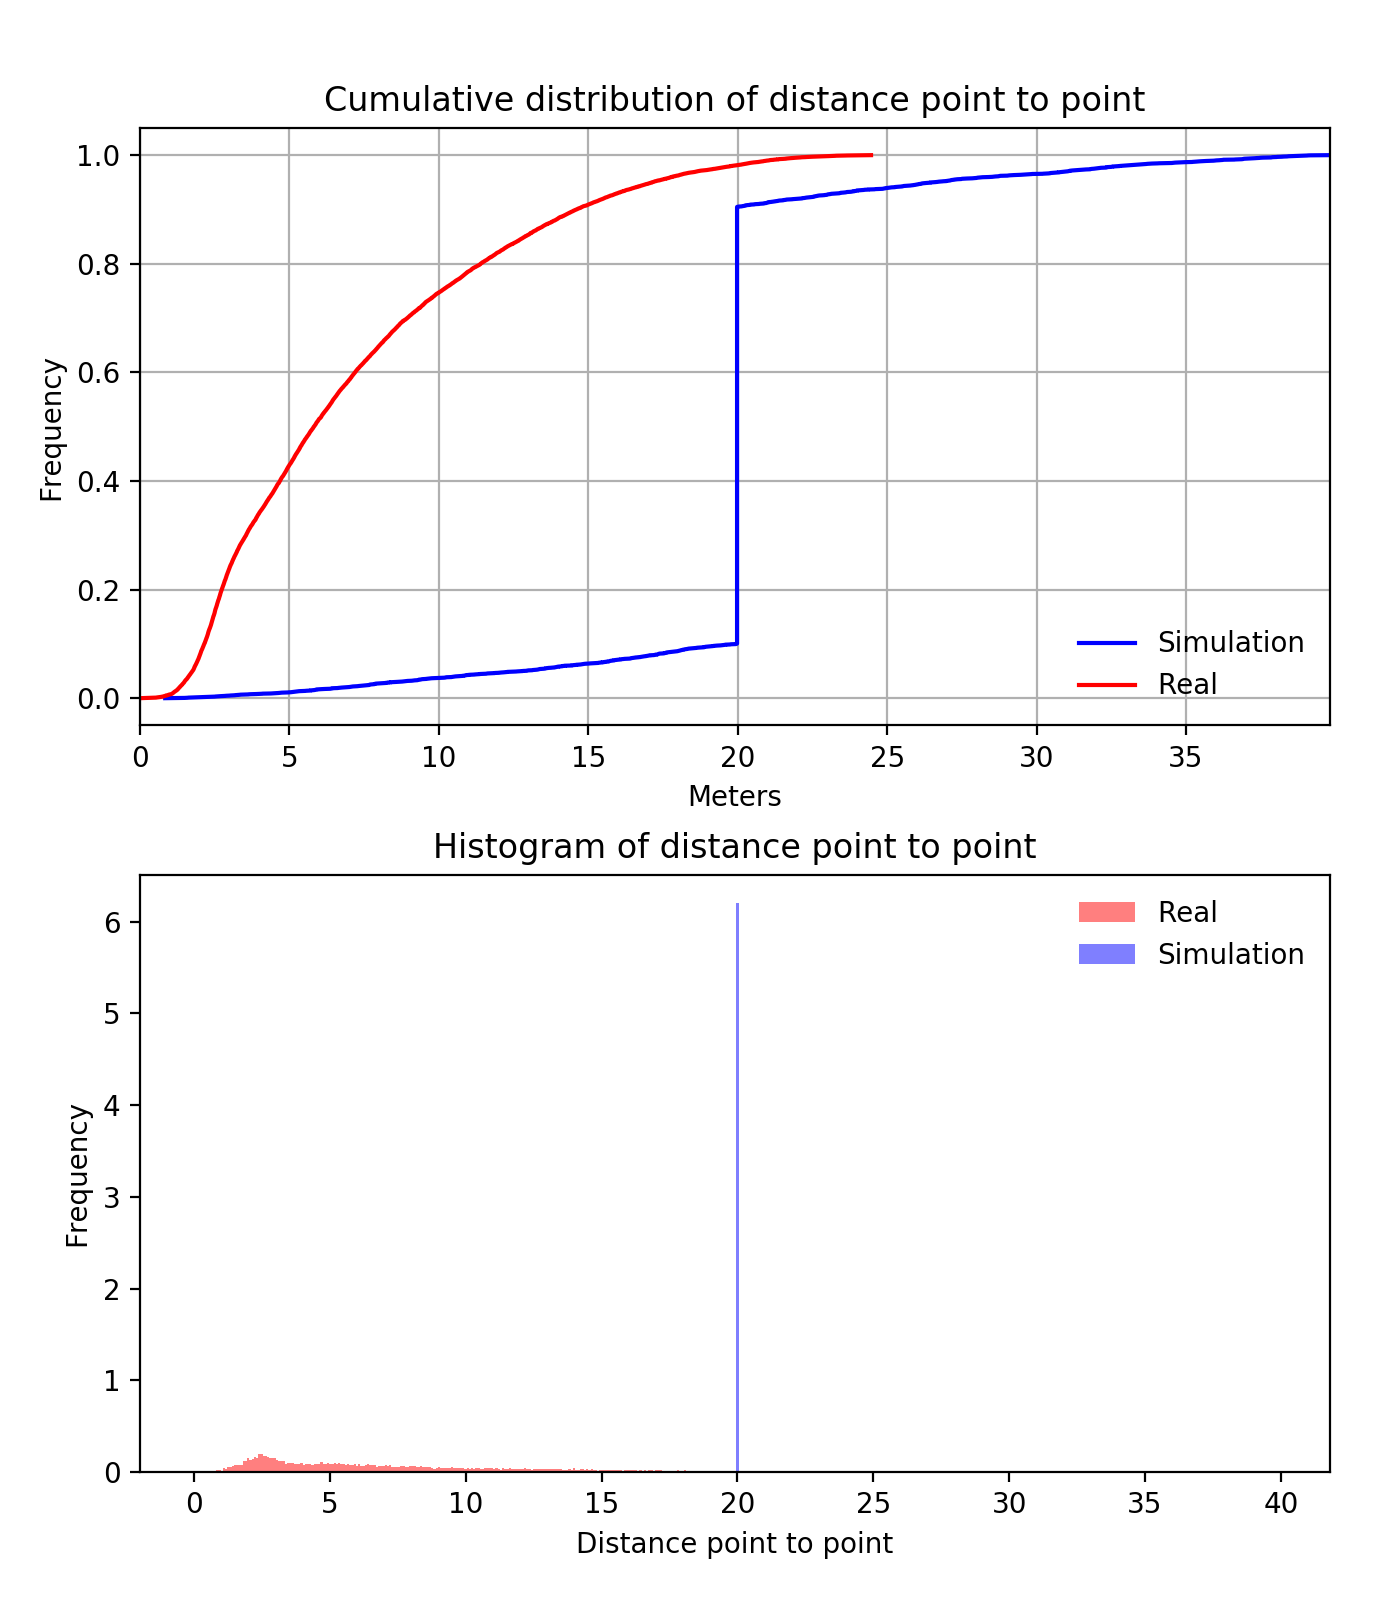
\includegraphics[width=1.2\textwidth]{./Imagenes/SimulationComparativeEmptyNormalized.png}
\caption{Comparativa análisis de la distancia punto a punto en simulación con datos.}
\label{figure:ComparativaEmpty}
\end{minipage}
\end{figure}
\newpage

Con esta información se aprecia que las simulaciones para este conjunto bajo de datos funciona con una alta similitud a las rutas reales proporcionadas.

\newpage
\newpage
\subsection{Anexo: Muestra de simulaciones con datos introducidos} \label{subseciton:SimulationSample}\begin{figure}[h]
\begin{center}
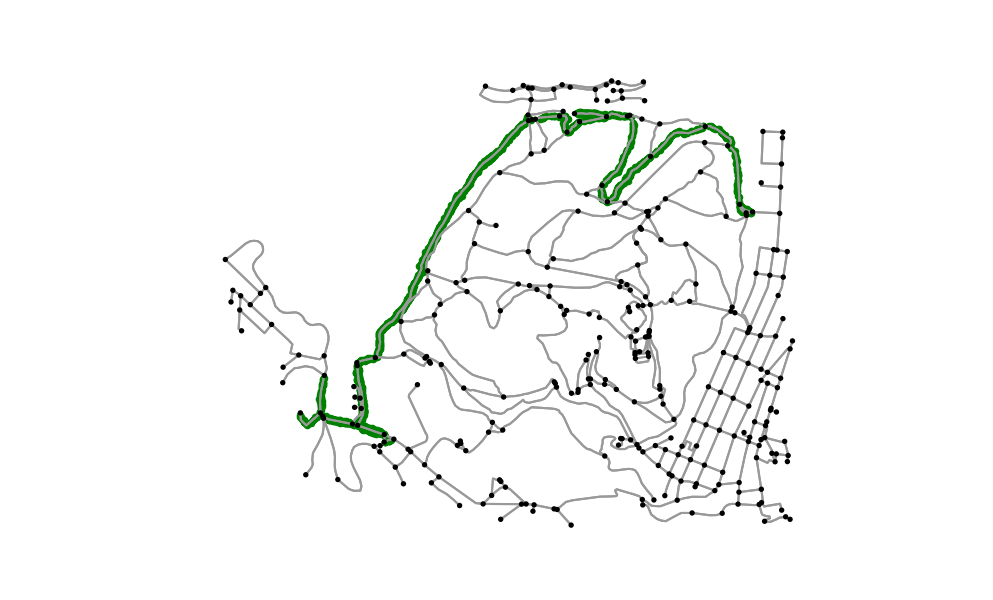
\includegraphics[width=0.95\textwidth]{./Imagenes/data-simulation/track1.png}
\caption{Simulación sin datos iniciales.}
\end{center}
\label{figure:Simulation1}
\end{figure}

\begin{figure}[h]
\begin{center}
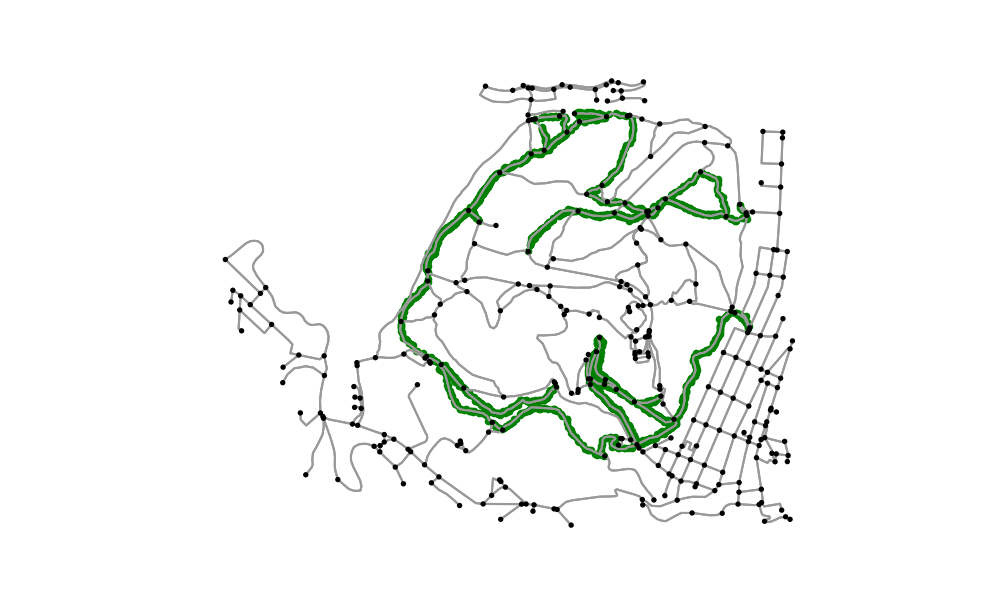
\includegraphics[width=0.95\textwidth]{./Imagenes/data-simulation/track2.png}
\caption{Simulación sin datos iniciales.}
\end{center}
\label{figure:Simulation2}
\end{figure}

\begin{figure}[h]
\begin{center}
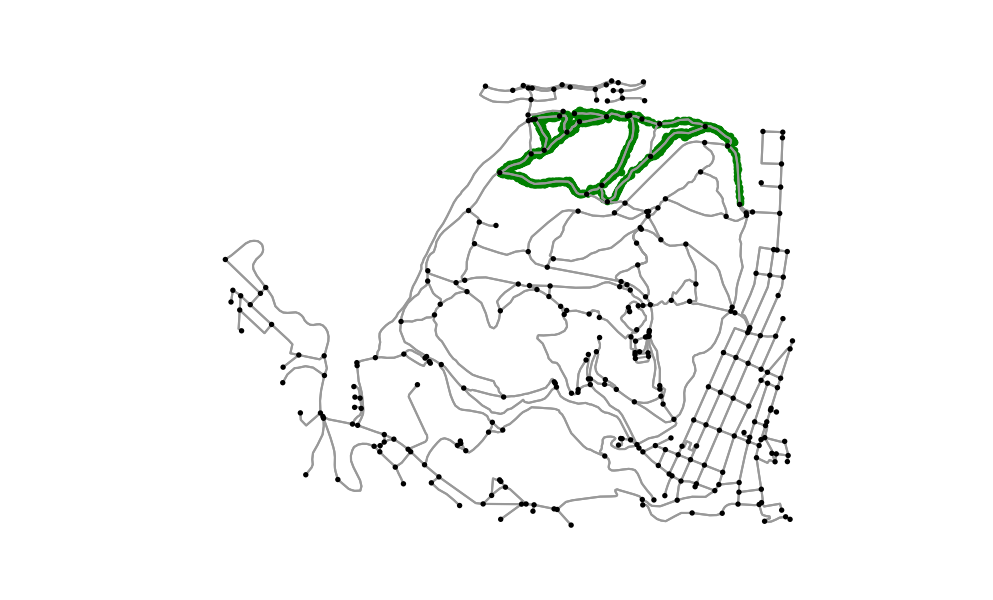
\includegraphics[width=0.95\textwidth]{./Imagenes/data-simulation/track3.png}
\caption{Simulación sin datos iniciales.}
\end{center}
\label{figure:Simulation3}
\end{figure}

\begin{figure}[h]
\begin{center}
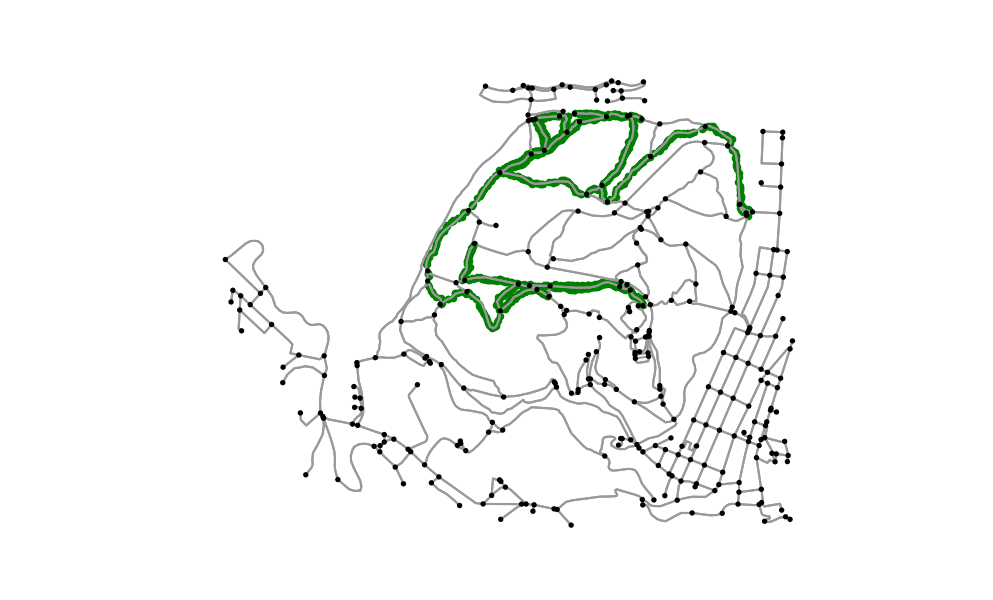
\includegraphics[width=0.95\textwidth]{./Imagenes/data-simulation/track4.png}
\caption{Simulación sin datos iniciales.}
\end{center}
\label{figure:Simulation4}
\end{figure}
\newpage

\subsection{Anexo: Muestra de simulaciones sin datos} \label{subseciton:SimulationSample}\begin{figure}[h]
\begin{center}
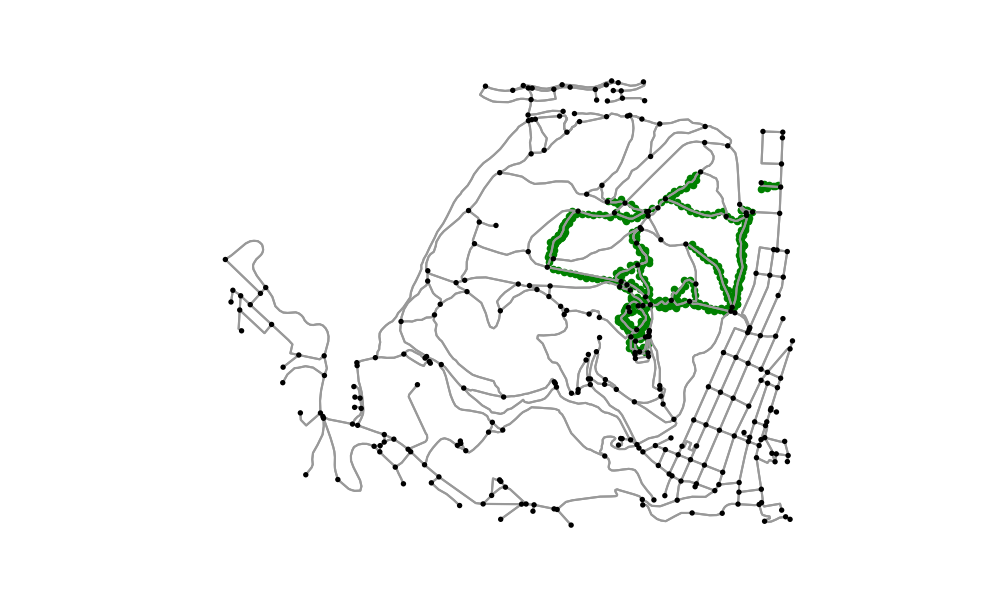
\includegraphics[width=0.95\textwidth]{./Imagenes/empty-simulation/track1.png}
\caption{Simulación sin datos iniciales.}
\end{center}
\label{figure:Simulation1}
\end{figure}

\begin{figure}[h]
\begin{center}
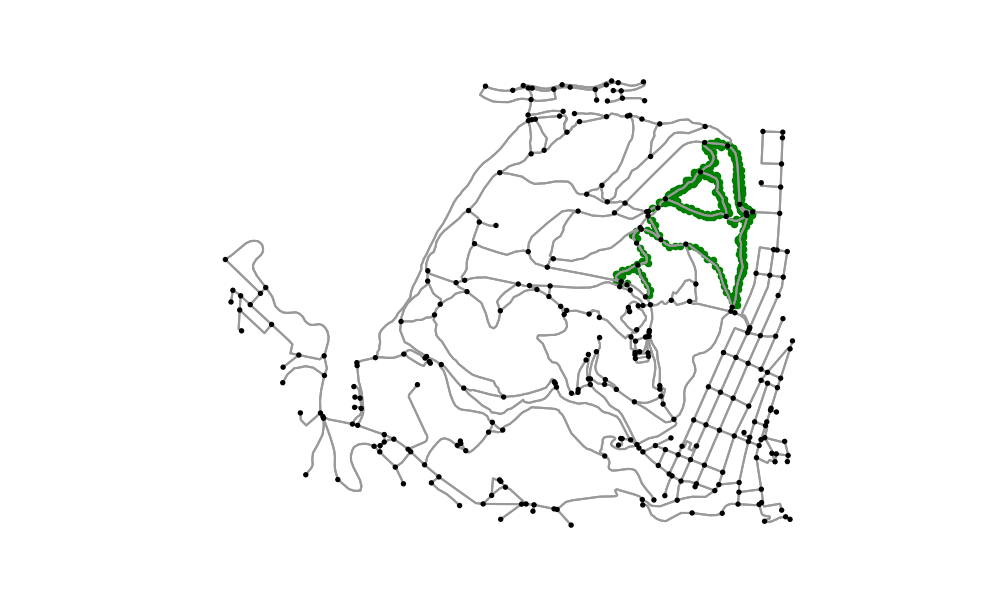
\includegraphics[width=0.95\textwidth]{./Imagenes/empty-simulation/track2.png}
\caption{Simulación sin datos iniciales.}
\end{center}
\label{figure:Simulation2}
\end{figure}

\begin{figure}[h]
\begin{center}
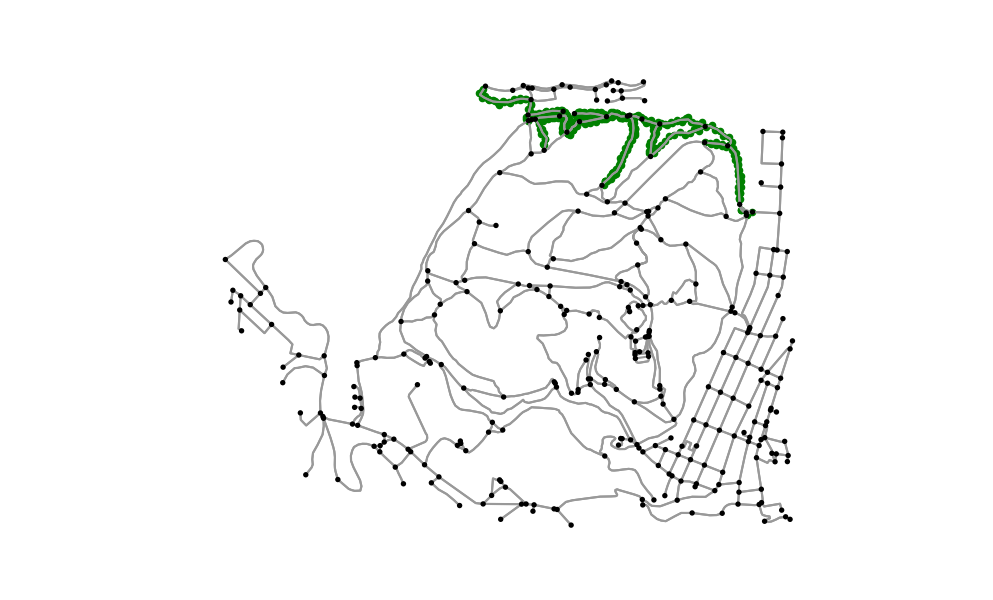
\includegraphics[width=0.95\textwidth]{./Imagenes/empty-simulation/track3.png}
\caption{Simulación sin datos iniciales.}
\end{center}
\label{figure:Simulation3}
\end{figure}

\begin{figure}[h]
\begin{center}
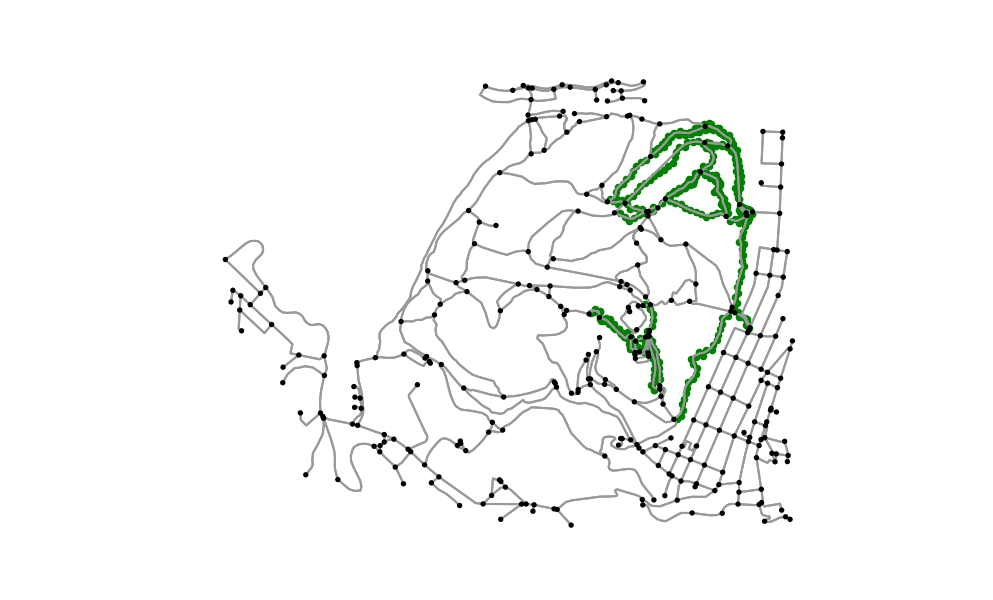
\includegraphics[width=0.95\textwidth]{./Imagenes/empty-simulation/track4.png}
\caption{Simulación sin datos iniciales.}
\end{center}
\label{figure:Simulation4}
\end{figure}
%!TeX root=MemoriaTFG.tex

\chapter{Guía de instalación y uso}
En esta sección se explicará como poder ejecutar la aplicación dentro de nuestro equipo, así como 
los comandos básicos para la ejecución de la aplicación.


%!TeX root=MemoriaTFG.tex

\chapter{Conclusiones}

En esta sección se realizará una explicará la opinión sobre el desarrollo de la propuesta.

\section{Posibles mejoras}
En esta sección se detallaran las posibles mejoras que se podrían implementar en la propuesta.


\section{Futuro trabajo}


\section{Opinión personal}

%%%%%%% Fi cos del treball %%%%%%%%%%%

% Si el vostre document no conté apèndixs 
% comentau les dues línies següents
%\appendix 
%%!TeX root=MemoriaTFG.tex

\chapter{Format final}

\section{Paper i impressió}

\subsection{Paper}

Cal utilitzar paper mida DIN A4 vertical (210 x 297 mm), el qual, a més de ser l'estàndard més generalitzat, és el format predeterminat de
la majoria de processadors de textos. No es recomana que el cos del TFG tengui una extensió superior a les 80 cares. Si la longitud del
treball és superior, s'hauria de pensar en passar informació cap als annexos.

\subsection{Impressió a dues cares}

La presentació del document ha de ser a dues cares a partir de la introducció i fins al final del document. Fixau-vos que la plantilla
\LaTeX\ ja produeix un document adequat per a la seva impressió a doble cara.

\section{Enquadernació}

Cal realitzar l'enquadernació amb espiral negra. Les tapes superior i inferior seran de plàstic transparent i negre, respectivament.

\section{La plantilla de \LaTeX}

La plantilla de \LaTeX\ d'aquest document defineix els marges, la tipografia, estils i espaiat de tots els elements per la memòria del treball de final de
grau. Una vegada es compila el document, \LaTeX\  adequarà el text al format definit en la plantilla. A més, \LaTeX\ realitzarà de forma
automàtica tot un seguit de funcions que us facilitaran la feina amb la memòria, com per exemple: numerar els capítols, seccions, i
sub-seccions; inserir els encapçalaments i números de pàgina; crear de forma automàtica els índexs de continguts, figures i taules \dots
Per tant, l'usuari només es preocuparà del text que està introduint, no serà necessari pensar en cap moment en l'aspecte final del
document. Serà \LaTeX\ qui aplicarà el format de la plantilla al teu text.

Aquesta plantilla està fonamentada en la classe \texttt{memoir}. Això presenta l'avantatge de que com que aquest format inclou automàticament altres \emph{packages}, per exemple \texttt{booktabs},
\texttt{array}, \texttt{tabularx}, etc., no caldrà carregar-los en el preàmbul del vostre document. Això també significa que totes les comandes de \texttt{memoir} estan a la vostra disposició per editar la memòria, per tant, és molt recomanable consultar el seu manual~\cite{Wil10}.

Amb el format de plantilla que s'ha definit només s'enumeraran 3 nivells de profunditat, a part dels capítols. Per definir-los s'utilitzaran les
següents expressions de \LaTeX:

\begin{verbatim}
\chapter{Nom del capítol}
\section{Nom de la secció}
\subsection{Nom de la sub-secció}
\subsubsection{Nom de la sub-sub-secció}
\end{verbatim}

\section{Fórmules, figures i taules}
\subsection{Fórmules}

El format de les fórmules es troba definit en la plantilla i \LaTeX\ l'aplica cada vegada que es compila el document.

Per escriure fórmules en \LaTeX\ s'hauran d'utilitzar les expressions adients. Aquí es presenta un exemple de codi:
\begin{verbatim}
\begin{equation}\label{NomEq}
\zeta= m \sum _{i=0}^{N} \left( \frac{\beta}{\sigma _i \lambda_ j}
\right)^{2} \cos (2\pi f_i)
\end{equation}
\end{verbatim}
que produeix el següent resultat:
\begin{equation}\label{NomEq}
\zeta= m \sum _{i=0}^{N} \left( \frac{\beta}{\sigma _i \lambda_ j}\right)^{2} \cos (2\pi f_i).
\end{equation}

Citar l'expressió anterior és tant senzill com fer:
\begin{verbatim}
L'equació \ref{NomEq} determina $\ldots$
\end{verbatim}
L'equació \ref{NomEq} determina $\ldots$

\subsection{Figures}

A continuació es mostra el codi \LaTeX\ per incloure una figura continguda en un fitxer.

\begin{verbatim}
\begin{figure}[htb]
\begin{center}

\includegraphics[width=0.2\textwidth]{./LogoUIB.jpg}
\caption{Exemple de figura}
\label{NomFig}
\end{center}
\end{figure}
\end{verbatim}
El resultat es pot veure a la Fig.~\ref{NomFig}.

\begin{figure}[htb]
\begin{center}

\includegraphics[width=0.2\textwidth]{./Imagenes/LogoUIB.jpg}
\caption{Exemple de figura}
\label{NomFig}
\end{center}
\end{figure}

Es pot modificar la variable \texttt{width} per ajustar l'amplada de la figura com més ens convingui. Teniu en compte que la variable
\texttt{\textbackslash textwidth} guarda el valor de l'amplada del text dins la pàgina i, per tant, és una bona referència per delimitar amplades de figura. Així doncs, la figura \ref{NomFig} ocupa la meitat de l'amplada del text en una pàgina. El format final de la figura està definit per la
plantilla i \LaTeX\ s'encarrega de presentar-la de forma convenient.

\subsection{Taules}

Les taules definides en \LaTeX\ s'enumeren automàticament i el format segueix les definicions especificades en la plantilla.

Seguidament, a mode d'exemple, es presenta les expressions \LaTeX\  per a crear
la taula \ref{NomTaula} que apareix més avall:
\begin{verbatim}
\begin{tabular}{@{}llS@{}} 
\toprule
\multicolumn{2}{c}{Cotxes} \\ 
\cmidrule(r){1-2}
{Posició} & {Descripció} & {Velocitat màxima}\\
 & &  \multicolumn{1}{s}{(\kilo\meter\per\second)} \\ 
\midrule
1 & Vermell & 120 \\
2 & Blau & 80.1 \\
3 & Verd & 92.50 \\
4 & Blanc & 33.33 \\
5 & Negre & 56.3 \\ 
\bottomrule
\end{tabular}
\caption{Exemple de taula} \label{NomTaula}
\end{table}
\end{verbatim}
\begin{table}
\centering
\begin{tabular}{@{}llS@{}} \toprule
\multicolumn{2}{c}{\textbf{Cotxes}} \\ 
\cmidrule(r){1-2}
{\textbf{Posició}} & {\textbf{Descripció}} & {\textbf{Velocitat màxima}}\\
 & &  \multicolumn{1}{s}{(\kilo\meter\per\second)} \\ \midrule
1 & Vermell & 120 \\
2 & Blau & 80.1 \\
3 & Verd & 92.50 \\
4 & Blanc & 33.33 \\
5 & Negre & 56.3 \\ \bottomrule
\end{tabular}
\caption{Exemple de taula} \label{NomTaula}
\end{table}

L'entorn \texttt{tabular} que ofereix \LaTeX\  és molt complet i permet crear
multitud de taules diferents, tot i que alhora és bastant complexe. No són les
intencions del present document descriure la sintaxis i el format d'aquest
tipus d'entorn. Es poden trobar molt fàcilment \emph{tutorials} o altres informacions
per aprendre a utilitzar de forma adient aquesta sintaxis o qualsevol altra de
\LaTeX. És bastant recomanable llegir la documentació del \emph{package}
\texttt{booktabs}\footnote{No cal incloure la comanda  \texttt{\textbackslash usepackage\{booktabs\}} dins el document perquè la classe ja ho fa.}~\cite{Fea05} on s'introdueixen una sèrie de comandes per a poder realitzar
taules de més qualitat com la de l'exemple, també es defineixen quines han de
ser les pautes per fer una taula d'aspecte formal. En aquest exemple concret també s'han usat les columnes \texttt{S} i \texttt{s} que ofereix el paquet \texttt{siunitx}~\cite{Wri12}. Un efecte similar es podria aconseguir amb les columnes de tipus \texttt{D} que inclou \texttt{memoir}~\cite[Cap. 11]{Wil10}.

Cal fixar-se en que \LaTeX\ insereix les figures i taules sempre al principi de pàgina. Per tant, no cal preocupar-se per la seva posició
dintre del document s'insereixen sempre en la mateixa posició de forma automàtica.

\section{Bibliografia}

A la bibliografia s'han de llistar conjuntament llibres i articles de revistes.
Citar una referència bibliogràfica és tant fàcil com fer:
\begin{verbatim}
\cite{bib1}, \cite{bib2}, \cite{bib3}
\end{verbatim}
per citar la referència \cite{bib1}, \cite{bib2}, \cite{bib3}. 

El format de la bibliografia es genera automàticament.

\section{Acrònims}

Per exemple, un acrònim ben conegut és l'\ac{IP}.
% Aquesta sentencia ens permetrà generar una entrada a la llista d'acrònims.
% En la llista d'acrònims es definiran cada un dels acronims i mitjançant l'expressió anterior podrem referenciar-los.
 

% En aquest cas sols hi ha un fitxer d'annexos,
% però podeu afegir tants \include com calgui. 

%%%%%%% Fi apèndix 

% No toqueu la línia següent 
\backmatter

% La comanda següent defineix l'estil bibliogràfic
\bibliographystyle{IEEEtran}

% La comanda següent defineix el fitxer que
% conté les referències bibliogràfiques.
% En aquest cas és el fitxer Bibliografia.bib
\bibliography{Bibliografia} 

\end{document}